\newcommand{\classname}{extbook}
\newcommand{\innermargin}{1.5cm}
\newcommand{\outermargin}{1.5cm}
\newcommand{\documentfontsize}{9pt}
\newcommand{\titlepagename}{dsp-titlepage}
\newcommand{\spacingvalue}{1.20}
\newcommand{\headsepvalue}{30pt}
\newcommand{\footskipvalue}{40pt}
\newcommand{\marginparsepvalue}{20pt}
\newcommand{\marginparwidthvalue}{90pt}

\documentclass[\documentfontsize, twocolumn]{\classname}
\usepackage[T1]{fontenc}
\usepackage[utf8]{inputenc}
\usepackage{amsmath,amssymb,amsfonts,bm}
\usepackage{amsthm}
\def\Z{\mathbb Z}
\def\R{\mathbb R}
\def\C{\mathbb C}
\def\N{\mathbb N}
\def\Q{\mathbb Q}

\DeclareMathOperator{\sinc}{sinc}
\DeclareMathOperator{\rect}{rect}
\DeclareMathOperator{\area}{area}
\DeclareMathOperator{\power}{power}
\DeclareMathOperator{\energy}{energy}
\DeclareMathOperator{\mval}{mval}


% Theorems
\newtheoremstyle{newlinethm}{2em}{2em}{\slshape}{2pt}{\bfseries}{\newline}{2em}{}
\theoremstyle{newlinethm}
\newtheorem{thm}{Theorem}[section]
\setlength{\tabcolsep}{0.5em} % for the horizontal padding
{\renewcommand{\arraystretch}{1.35}% for the vertical padding

\newtheorem{predicate}{Predicate}[section]
\setlength{\tabcolsep}{0.5em} % for the horizontal padding
{\renewcommand{\arraystretch}{1.35}% for the vertical padding

\newtheorem{rules}{Rule}[section]
\setlength{\tabcolsep}{0.5em} % for the horizontal padding
{\renewcommand{\arraystretch}{1.35}% for the vertical padding

\theoremstyle{theorem}
\newtheorem{lemma}{Lemma}[section]
\setlength{\tabcolsep}{0.5em} % for the horizontal padding
{\renewcommand{\arraystretch}{1.35}% for the vertical padding

\newtheorem{tesi}{Tesi}[section]
\setlength{\tabcolsep}{0.5em} % for the horizontal padding
{\renewcommand{\arraystretch}{1.35}% for the vertical padding

\theoremstyle{definition}
\newtheorem{defin}{Definition}[section]
\setlength{\tabcolsep}{0.5em} % for the horizontal padding
{\renewcommand{\arraystretch}{1.35}% for the vertical padding

\theoremstyle{definition}
\newtheorem{regola}{Regola}[section]
\setlength{\tabcolsep}{0.5em} % for the horizontal padding
{\renewcommand{\arraystretch}{1.35}% for the vertical padding

\theoremstyle{definition}
\newtheorem{identita}{Identità}[section]
\setlength{\tabcolsep}{0.5em} % for the horizontal padding
{\renewcommand{\arraystretch}{1.35}% for the vertical padding

\theoremstyle{definition}
\newtheorem{predicato}{Predicato}[section]
\setlength{\tabcolsep}{0.5em} % for the horizontal padding
{\renewcommand{\arraystretch}{1.35}% for the vertical padding

\renewcommand\proofname{\textup{\emph{Proof.}}} % default is 'Proof.' 
\renewcommand\qedsymbol{$\blacksquare$}

\newcommand\encircle[1]{%
    \hspace*{2pt}\tikz[baseline=(X.base)] 
    \node (X) [draw, shape=circle, inner sep=-2.5pt, minimum size=0pt] {\strut \footnotesize #1};\hspace*{2pt}}

\usepackage{color}
\usepackage{listings}
\definecolor{dkgreen}{rgb}{0.1,0.5,0.1}
\definecolor{greengray}{rgb}{0.517,0.761,0.404}
\definecolor{orange}{rgb}{0.717,0.274,0.105}
\definecolor{blue}{rgb}{0.164,0.317,0.600}
\definecolor{background}{rgb}{0.990,0.990,0.990}
\lstset {
	frame=lrtb,
	language=java,
	aboveskip=0.7cm,
	belowskip=0.2cm,
	showstringspaces=false,
	columns=flexible,
	basicstyle={\small\ttfamily},
	numbers=none,
	backgroundcolor=\color{background},
	numberstyle=\tiny\color{dkgreen},
	keywordstyle=\color{blue},
	commentstyle=\color{greengray},
	stringstyle=\color{orange},
	breaklines=true,
	breakatwhitespace=true,
	tabsize=3
}

\usepackage{tikz}
\usepackage{pgfplots}
\usetikzlibrary{circuits}
\usetikzlibrary{positioning}
\usetikzlibrary{shapes.geometric}
\usetikzlibrary{decorations.markings}
\usetikzlibrary{arrows.meta}
\usetikzlibrary{decorations.pathreplacing,angles,quotes,calligraphy}
\tikzset{squarednode/.style={rectangle, draw=black!90, fill=black!10, very thick, minimum size=5mm}}
\tikzset{boxfilter/.style={rectangle, draw=black!90, thick, minimum width=.7 cm, minimum height=.5cm}}
\tikzset{dot/.style={inner sep=1pt, fill=black!100, circle}}
\tikzset{cross/.style={path picture={ \draw[black] (path picture bounding box.south east) -- (path picture bounding box.north west) (path picture bounding box.south west) -- (path picture bounding box.north east);}}}
\tikzset{plus/.style={path picture={ \draw[black] (path picture bounding box.south) -- (path picture bounding box.north) (path picture bounding box.east) -- (path picture bounding box.west);}}}
\tikzset{multiplierdownwards/.style={isosceles triangle, isosceles triangle apex angle=100, rotate=270, thick, minimum size=.35cm}}
\tikzset{-dot-/.style={decoration={ markings, mark=at position #1 with {\fill circle (1pt);}},postaction={decorate}}} %%% in this line added a ;

\usepackage{upgreek}
\def\alpha{\upalpha}
\def\beta{\upbeta}
\def\delta{\updelta}
\def\epsilon{\upepsilon}
\def\gamma{\upgamma}
\def\kappa{\upkappa}
\def\lambda{\uplambda}
\def\mu{\upmu}
\def\omega{\upomega}
\def\phi{\upphi}
\def\pi{\uppi}
\def\psi{\uppsi}
\def\rho{\uprho}
\def\tau{\uptau}
\def\theta{\uptheta}
\def\upsilon{\upupsilon}
\def\varepsilon{\upvarepsilon}
\def\varphi{\upvarphi}
\def\xi{\upxi}

\usepackage{pgfplots}
\usepackage{fontspec}
%\usepackage{mlmodern}
\usepackage[default,regular,black]{sourceserifpro}
\usepackage[stickstoo]{newtxmath}
%\usepackage[p]{scholax}
%\usepackage[scaled=1.075,ncf]{newtxmath}
%\usepackage[nomath,variablett]{lmodern}
%\usepackage[usefilenames,DefaultFeatures={Ligatures=Common}]{plex-otf} %
%\usepackage{stickstootext}
%\usepackage[libertine]{newtxmath}
%\usepackage{erewhon}
%\usepackage{times}
%\usepackage[scaled=0.92]{CharisSIL}
%\usepackage[charter]{mathdesign}
%\usepackage{tgschola}
%\usepackage[scaled=1.000,ncf,vvarbb]{newtxmath}
%\usepackage{mathpazo}
%\usepackage[libertine]{newtxmath}
\usepackage[all]{nowidow}
\usepackage{graphicx}
\usepackage{svg}
\usepackage[pdfa]{hyperref}
\usepackage{makecell}
\usepackage{setspace}
\usepackage{parskip}
\setcounter{MaxMatrixCols}{20}
\usepackage[a4paper, inner=\innermargin, outer=\outermargin]{geometry}

\setlength{\columnsep}{42pt}
\font \monofontfs = "IBM Plex Mono"

\begin{document}
\setmonofont[Scale=0.9]{IBM Plex Mono}
\include{\titlepagename}
%\title{\Huge \textsc{Digital Signal Processing}}
%\author{\large \emph{Marco Sgobino}}
%\maketitle
\setstretch{\spacingvalue}
\setlength{\emergencystretch}{0pt}
\pretolerance=150
\tolerance=250
\hbadness=150
\hfuzz=0pt
\setlength{\headsep}{\headsepvalue}
\setlength{\footskip}{\footskipvalue}
\setlength{\marginparsep}{\marginparsepvalue}
\setlength{\marginparwidth}{\marginparwidthvalue}

\tableofcontents

% Teacher's email: ramponi at units dot it, office C2_1.25
%
% Suggested book: - S.K. Mitra, "Digital Signal Processing: A Computer-Based Approach", McGraw-Hill 2006 (3rd ed.) - 2011 (4th ed.)

\part{Discrete Time Systems}

\chapter{Time-Domain Representation of Discrete-time Signals}

\textbf{Time domain} refers to the analysis of mathematical functions, physical
signals or time series of economic or environmental data, with respect to
\emph{time}. In the time domain, the signal or function's value is known for
all real numbers, for the case of continuous time, or at various separate
instants in the case of discrete time. An oscilloscope is a tool commonly used
to visualize real-world signals in the time domain. A time-domain graph shows
how a signal changes with time, whereas a fre\-quen\-cy-do\-ma\-in graph shows
how much of the signal lies within each given frequency band over a range of
frequencies.

Though most precisely referring to time in physics, the term time domain may
occasionally informally refer to position in space when dealing with spatial
frequencies, as a substitute for the more precise term spatial domain~\cite{bib:wikiTimeDomain}.

\section{Signal definition}

In signal processing, a \textbf{signal} is a function that conveys information
about a phenomenon. Signals are functions of independent variables, such as
\emph{time}, \emph{distance}, \emph{position}, and so on. They are represented
as se\-quen\-ces of numbers, called \emph{samples}. Signals are composed of
samples---the single values of the signal at a certain, discrete time quantum $n
\in \Z$. Signals will be denoted with $\{x[n]\}$ while samples will be denoted
as $x[n]$. The variable $n$ may or may not be an integer, since the quantum of
time may not be constant in some applications.

Typically a discrete signal can be either a \emph{sampled-data signal} or a
\emph{digital} signal. Both types of signals only exist in specific time quanta
and they are likely the result of a sampling, but only digital signals have
\emph{quantized} value---common sampled-data signals will possess continuous
values. Values of digital signals are usually obtained from sample values
either by \emph{rounding} or \emph{truncation} techniques---in both cases an
error occurs.

Since signals can have multiple time domains, one has to clarify when
equivalences between amplitudes may apply. In particular, the following
relationship \[ x[n] = \left.x_a(t)\right|_{t=nT} = x_a(nT), n \in \Z\]
yields only as long as we do not take in account any \emph{quantization error},
since---by definition---digital signals are the result of both a sampling process
and a quantization process. The spacing between two samples is said to be
\emph{sampling interval} or \emph{sampling period} and measures in seconds,
and the reciprocal of such quantity is called \emph{sampling frequency} $F_T$
or $F_S$ and measures in Hertz.

\section{Basic signal properties}

\subsubsection{Nature of signals}

Signals can be either \emph{deterministic} or \emph{random}; the first case
denotes a signal that can be inferred by some rule or formula, while a random
signal cannot be generally predicted ahead of time. Examples of random signals
are the \emph{stock exchange}, or the \emph{coin flip}. Random signals are
usually considered as they are generated in a random fashion---even though
there might exist some actual underlying rule we don't actually know.

\subsubsection{Filters}

A \emph{filter} is a system which \emph{is able to control the frequency
content of the output with respect to the input signal}. When a filter is
\emph{linear}, the output of the filtering operation sums up to the
\emph{convolution} operation, which is the following signal,
\[
y(t) = \int_0^T x(t - \tau)h(\tau)d\tau.
\]
The role of $\tau$ in the convolution is to shift-reverse one of the two
signals, while the multiplication with the other signal occurs. This ensures
that the overall result will be a new signal which is the sum,
sample-to-sample, between one of the two signals in its original form and a
``moving'' shift-reversed form of the other one.

\subsubsection{Visual representation of a signal}

A signal can be also represented as a se\-quen\-ce of values inside brackets. To
denote where the time instant $0$ is, an arrow is placed below the sample of the
se\-quen\-ce corresponding to $n=0$. As an example, the following notation can express a signal:
\[ \{x[n]\} = \{\dots, -0.2,1,\underset{\uparrow}{3},-6.7,-5.4,0.1,3.6,1.2,\dots\}\] and, with this notation, $x[0]=3$.

To represent signals, a \emph{stem plot} is usually adopted. There are two
different forms of stem plot: a first one in which only samples are
represented---dots along with their straight vertical line denoting the
\emph{amplitude} of the signal in such quantum of time---and another one in
which superposed to the samples an analog-like line is represented. In the
latter case, there may be two different interpretations; either the digital
signal is sampled from an original analog signal, or the continuous line
denotes the amplitude of the digital signal \emph{as if} it were analog.

\begin{figure}[ht]
\begin{center}
\scalebox{0.6}{
% Title: gl2ps_renderer figure
% Creator: GL2PS 1.4.2, (C) 1999-2020 C. Geuzaine
% For: Octave
% CreationDate: Wed Oct 19 08:50:18 2022
\setlength{\unitlength}{1pt}
\begin{picture}(0,0)
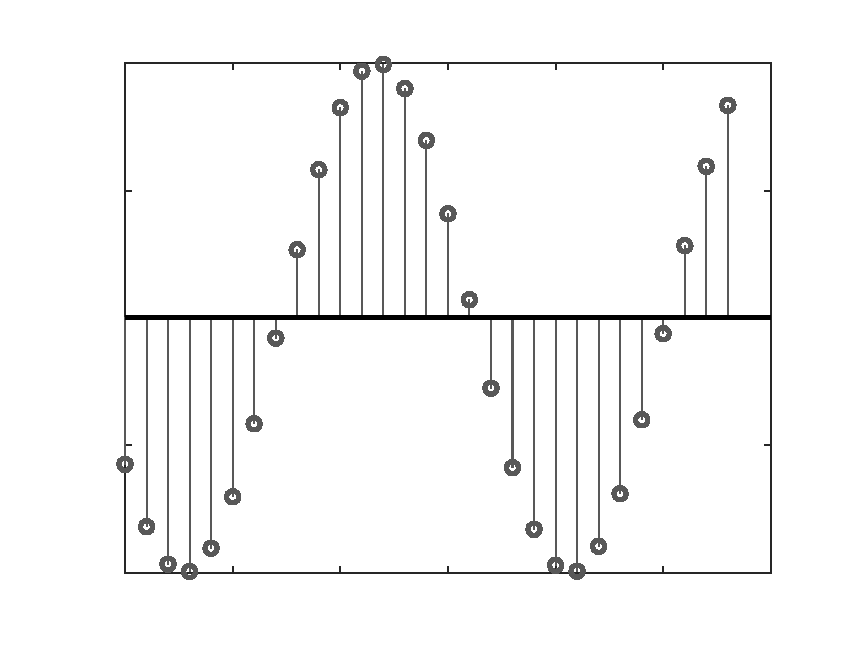
\includegraphics[scale=1]{octaves/stem-plot-inc}
\end{picture}%
\begin{picture}(400,300)(0,0)
\fontsize{6}{0}\selectfont\put(52,27.8){\makebox(0,0)[t]{\textcolor[rgb]{0.15,0.15,0.15}{{-10}}}}
\fontsize{6}{0}\selectfont\put(103.667,27.8){\makebox(0,0)[t]{\textcolor[rgb]{0.15,0.15,0.15}{{-5}}}}
\fontsize{6}{0}\selectfont\put(155.333,27.8){\makebox(0,0)[t]{\textcolor[rgb]{0.15,0.15,0.15}{{0}}}}
\fontsize{6}{0}\selectfont\put(207,27.8){\makebox(0,0)[t]{\textcolor[rgb]{0.15,0.15,0.15}{{5}}}}
\fontsize{6}{0}\selectfont\put(258.667,27.8){\makebox(0,0)[t]{\textcolor[rgb]{0.15,0.15,0.15}{{10}}}}
\fontsize{6}{0}\selectfont\put(310.333,27.8){\makebox(0,0)[t]{\textcolor[rgb]{0.15,0.15,0.15}{{15}}}}
\fontsize{6}{0}\selectfont\put(362,27.8){\makebox(0,0)[t]{\textcolor[rgb]{0.15,0.15,0.15}{{20}}}}
\fontsize{6}{0}\selectfont\put(48.5263,33){\makebox(0,0)[r]{\textcolor[rgb]{0.15,0.15,0.15}{{-1}}}}
\fontsize{6}{0}\selectfont\put(48.5263,94.125){\makebox(0,0)[r]{\textcolor[rgb]{0.15,0.15,0.15}{{-0.5}}}}
\fontsize{6}{0}\selectfont\put(48.5263,155.25){\makebox(0,0)[r]{\textcolor[rgb]{0.15,0.15,0.15}{{0}}}}
\fontsize{6}{0}\selectfont\put(48.5263,216.375){\makebox(0,0)[r]{\textcolor[rgb]{0.15,0.15,0.15}{{0.5}}}}
\fontsize{6}{0}\selectfont\put(48.5263,277.5){\makebox(0,0)[r]{\textcolor[rgb]{0.15,0.15,0.15}{{1}}}}
\fontsize{7}{0}\selectfont\put(207,287.5){\makebox(0,0)[b]{\textcolor[rgb]{0,0,0}{{A stem plot of a sinusoidal sequence}}}}
\end{picture}

}\caption{\emph{Stem plot} of a sinusoidal function. In particular, a stem plot of \texttt{cos(.35*x - .6)} has been performed with the help of the \texttt{octave} CLI. Pre-built binaries of the program are available at their website \texttt{https://octave.org/}.}\label{oct:stemPlot}
\end{center}
\end{figure}

Two kinds of digital signal representation exist. The first type is the common
digital signal where each sample is represented with a dot and a straight
line, while a \emph{boxedcar} signal will see each sample represented as a
straight line, in a similar fashion to the interpolation.

\subsubsection{Complex signals}

A signal can be either real or complex valued. A \emph{real se\-quen\-ce} comprises
only real samples such that $x[i] \in \R, \forall i \in \Z$ while a
\emph{complex se\-quen\-ce} has at least one complex sample $x[k] \in \C$. Complex
se\-quen\-ces may be seen as the result of the sum of two, distinct, real
se\-quen\-ces. In particular, by writing \[\{x[n]\} = \{x_{re}[n]\} +
j\{x_{im}[n]\}\] two different se\-quen\-ces, one for real part and the other one
for the imaginary part, are summed to form a single complex signal. It's easy
to understand that a real valued signal can still be written as a complex
signal, provided that $x_{im}[n] \equiv 0, \forall n$.

A complex signal's short, alternative notation is \[\{x[n]\} = \{A[n]e^{-j\cdot
f_t n}\},\] where the imaginary and real part are intrinsic in the exponential
representation and can thus be obtained by decomposing it into a sine and a
cosine addenda.

\subsubsection{Length of a signal}

A signal can either be of \emph{finite} or \emph{infinite}-length. In the first case defined values for the se\-quen\-ce lay only in an interval $N_1 \leq n \leq N_2$, with $N_1 \leq N_2$ and both $-\infty < |N_1| \leq |N_2| < \infty$. The overall \emph{length} or \emph{duration} of the se\-quen\-ce will be $N = N_2 - N_1 + 1$. In the second case a se\-quen\-ce is defined for every value of $n \in \Z$, after a certain $n_0$. For instance, $\{\cos{f_0 n}\}$ is an infinite-length se\-quen\-ce, because the signal ``never ends'', as there is no $n_1$ after which or before which the signal is null. Other infinite-length signals are any signal defined for all values after an $n_0 \in \Z$.

In practice, no signal really has infinite length, but it could be useful to still think of signals as such to make them more mathematically treatable.

\subsubsection{Zero-padding}

A signal may see its length varied by arbitrary operations. A very common operation in that regard, is to increase the length of a signal by appending or prepending $0$s to the signal, with a process called \textbf{zero-padding}. This usually involves a finite-length signal becoming an infinite-length signal by applying an infinitely long list of $0$s on both sides of the original signal; it is not uncommon, however, to apply the zero-padding technique to only one side of the signal. Another way to handle zero-padding is to simply add a finite---yet necessary---number of $0$s depending on the duty to perform.

\subsubsection{Causality}

A se\-quen\-ce is said to be \emph{right-sided} if it has zero-valued samples for each $n < N_1$. A special case of right-sided se\-quen\-ce is when $N_1 \geq 0$, the case of a \textbf{causal} signal.

Vice-versa, a se\-quen\-ce is said to be \emph{left-sided} if it has zero-valued samples for each $n > N_2$. The same way, when a left-sided se\-quen\-ce has $N_2 \leq 0$, we are in the case of an \textbf{anti-causal} signal.

Basically, causal signals are all signals that ``are relevant only \emph{after} a certain time $N_1$'', and anti-causal signals are all signals that ``are relevant \emph{before} a given time $N_2$''.

\subsubsection{Strength of a signal and signal comparison}

An important concept is the \textbf{strength} of a signal, also called \emph{size} of a signal. The strength of a signal is the $\mathcal{L}_p$-norm of the se\-quen\-ce,
\[
||x||_p = \left(\sum_{i=N_1}^{N_2} |x[n]|^p\right)^{\frac{1}{p}},
\]
where $p \in \N \setminus \{0\}$ is a positive integer, which is different from zero. Typically, one has $p=1,2,\infty$, with $p=2$ being the \emph{root mean squares} apart from a scaling factor---RMS is the square root of the \textbf{mean} of the squares, there's an additional $\frac{1}{\sqrt{n}}$ factor. The other two cases are $p=1$ corresponding to the \emph{mean absolute value} of the signal---except from a constant factor---and $p=\infty$ where the strength of the signal would be the \emph{absolute peak value} of the signal.

From the concept of signal strength the concept of \emph{relative error} immediately follows. In particular, let $\{y[n]\}, 0 \leq n \leq N - 1$ be an approximation of the signal $\{x[n]\}, 0 \leq n \leq N - 1$. In this case, one calls relative error the quantity
\begin{equation}\label{eqn:RelativeError}
	E_{rel} = \left(\frac{\sum_{n=0}^{N-1} |y[n] - x[n]|^2}{\sum_{n=0}^{N-1} |x[n]|^2}\right)^\frac{1}{2},
\end{equation}
which is the ratio of the $\mathcal L_2$-norm of the difference signal and the $\mathcal L_2$-norm of the signal $\{x[n]\}$. Everything is square-rooted.

The numerator of such quantity can be considered as the error between se\-quen\-ces $x$ and $y$, while the denominator is the $2$-strength of a non-approximated se\-quen\-ce.

\subsection{Operations on se\-quen\-ces}\label{sec:operationsOnSequences}

se\-quen\-ces may be subjected to \emph{operations}. In particular, operations can be described by directed graphs in which there is an input se\-quen\-ce and an output se\-quen\-ce resulting from the operation. Of course, there may be more than one inputs or outputs.

    \begin{figure}[ht]
\begin{center}
\begin{tikzpicture}

    \node                 (input)                                 {$\{x[n]\}$};
    \node[squarednode]    (operation)     [right=of input]        {Operation};
    \node                 (output)        [right=of operation]    {$\{y[n]\}$};

    \draw[->] (input.east) -- (operation.west);
    \draw[->] (operation.east) -- (output.west);
\end{tikzpicture}\caption{The general scheme for elementary operations.}\label{tikz:operation-scheme}
\end{center}
\end{figure}

Basic signal operations are called \textbf{elementary operations}. The first
elementary operation is the \emph{modulation}, an operation in which a signal
$x$ is multiplied by another signal, say $w$, to produce an output signal $y$
such that $$y[n] = x[n]\cdot w[n].$$ A common application of the modulation is
the \emph{windowing} process, in which an infinite-length signal $x$ is
``windowed'' by a finite-length signal $w$, whose non-zero values are limited
to a finite interval and the non-zero values are all equal to $1$. In that
case, it would be like ``selecting'' the values of $x$ that lay in the $w$
window. Modulation is denoted with a cross inside a circle, as shown in Diagram~\ref{tikz:modulation-operation}.

\begin{figure}[ht]
\begin{center}
    \begin{tikzpicture}
    \node [](A){$x[n]$};
    \node [draw, fill=purple!15,circle,cross, thick,minimum width=0.5 cm](B) at (1,0){}; 
    \node [](C) at(2,0){$y[n]$}; 
    \node [](D) at(1,-1){$w[n]$}; 
    \draw[->] (A) -- (B);
    \draw[->] (B) -- (C);
    \draw[->] (D) -- (B);
\end{tikzpicture}\caption{Notation for the modulation (product) operation.}\label{tikz:modulation-operation}
\end{center}
\end{figure}

Other elementary operations are the \emph{multiplication} operation and the \emph{addition} operation. The multiplier is denoted by a triangle---an opamp-like symbol is adopted---while the addition is a plus symbol inside a circle. Diagrams~\ref{tikz:multiplication-operation} and~\ref{tikz:addition-operation} summarize the overall notation. This time, multiplication is not performed between entire signals, but instead a constant $A$ multiplies a signal $x$, such that $$y[n] = A \cdot x[n].$$ The addition is performed between two distinct signals, hence $$z[n] = x[n] + y[n].$$

\begin{figure}[ht]
\begin{center}
    \begin{tikzpicture}
    \node [](A){$x[n]$};
    \node [draw, fill=red!10,isosceles triangle,thick,minimum width=.4 cm](B) at (1.5,0){$A$}; 
    \node [](C) at(3,0){$y[n]$}; 
    \draw[->] (A) -- (B);
    \draw[->] (B) -- (C);
\end{tikzpicture}\caption{Notation for the multiplication (product for a constant) operation.}\label{tikz:multiplication-operation}
\end{center}
\end{figure}

\begin{figure}[ht]
\begin{center}
\begin{tikzpicture}
    \node [](A) at (0,0){$x[n]$};
    \node [draw, fill=green!15,circle,plus,thick,minimum width=.5 cm](B) at (1,0){}; 
    \node [](C) at(2,0){$z[n]$}; 
    \node [](D) at(1,-1){$y[n]$};
    \draw[->] (A) -- (B);
    \draw[->] (B) -- (C);
    \draw[->] (D) -- (B);
\end{tikzpicture}\caption{Notation for the addition (sum) operation.}\label{tikz:addition-operation}
\end{center}
\end{figure}

Much relevant elementary operations are, indeed, the \emph{time delay} and
\emph{time advance}. A signal that is time-delayed is a signal which is a copy
of the original signal, but translated in time (delayed in this case).
Vice-versa, in the case of time advance, the signal copy of the original will be
anticipated. In the first case, the adopted symbol is $z^{-1}$, while for the
anticipation it is $z$. Hence, $y[n] = x[n - 1]$ and $y[n] = x[x + 1]$.

\begin{figure}[ht]
\begin{center}
    \begin{tikzpicture}
    \node [](A){$x[n]$};
    \node [draw, fill=red!10,boxfilter](B) at (1.5,0){$z^{-1}$}; 
    \node [](C) at(3,0){$x[n-1]$}; 
    \draw[->] (A) -- (B);
    \draw[->] (B) -- (C);
\end{tikzpicture}\caption{Notation for the time delaying operation.}\label{tikz:delaying-operation}
\end{center}
\end{figure}

\begin{figure}[ht]
\begin{center}
    \begin{tikzpicture}
    \node [](A){$x[n]$};
    \node [draw, fill=red!10,rectangle,thick,minimum width=.7 cm, minimum height=.5cm](B) at (1.5,0){$z$}; 
    \node [](C) at(3,0){$x[n+1]$}; 
    \draw[->] (A) -- (B);
    \draw[->] (B) -- (C);
\end{tikzpicture}\caption{Notation for the time advance operation.}\label{tikz:advance-operation}
\end{center}
\end{figure}

An interesting operation is the \emph{time reversal} or \emph{folding}. The folding operation inverts the time axis of a signal, that means $y[n] = x[-n]$. Time reversal does not have any explicit symbol, since it requires a complete reflection of a signal from its origin point.

Yet another common `operation' is the \emph{branching} operation, in which a signal $w$ is simply the copy of the input signal, as well as the $y$ signal (a single input is copied into two outputs). Branching is shown in Diagram~\ref{tikz:branchingOperation}.
\begin{figure}[ht]
\begin{center}
    \begin{tikzpicture}
    \node [](A){$x[n]$};
    \node [draw, fill=black!100,inner sep=1pt,circle,label=above:{b}](B) at (1.5,0){}; 
    \node [](C) at(3,0){$x[n]$}; 
    \node [](D) at(1.5,-1.5){$x[n]$}; 
    \draw[->] (A) -- (B) -- (C);
    \draw[->] (B) -- (D);
\end{tikzpicture}\caption{Notation for the branching (signal splitting) operation. The $b$ node allows splitting of the signal into two---equal---branches where $x$ is routed.}\label{tikz:branchingOperation}
\end{center}
\end{figure}

In order to apply most of the above operations, two signals should possess the same length---in those cases where this does not occur, a \emph{zero-padding} is required. For instance, to perform addition on two signals, the two signals must share the same length, therefore it is mandatory to at least perform a zero-padding on the shortest of the signals. Infinitely long signals can always be summed together.

Multiple elementary operations can be combined as well, by building a directed graph in which the signals are subjected to multiple eventual operations, in the order determined by the particular graph. Usually, multiple operations should be necessary and are therefore applied in special manners to obtain the desired result.

\section{Ensemble Averaging}

A very powerful operation to apply to a signal is the \textbf{ensemble averaging}. Ensemble averaging is the operation of performing an average of a signal when multiple, independent measures are available. The goal of the ensemble averaging is to enhance the quality of a signal with respect to a noise which affects it. In other words, the result is expected to suffer less from noise than the original signal.

Suppose $i$-th measured signal $x_i$ has two components $x_i = s + d_i$, the
first one relative to an original signal $s$ and the noise component $d_i$, which
varies according to the measurement. The ensamble average of the $K$ measurements is the signal $x_{avg}$ such that
\begin{equation}\label{eqn:EnsambleAveraging}
	x_{avg} = \frac{1}{K}\sum_{i=1}^{K} s + d_i = s + \frac{1}{K}\sum_{i=1}^{K}d_i,
\end{equation}
which tends to the original signal $s$ as the number of signals $K \rightarrow \infty$ approaches infinity. The benefit of the ensemble averaging lies in the fact that the variance of the white noise $d_i$ is reduced by a factor of $K$, leading to a reasonable replica of the original signal $s$. An example of application of ensemble averaging is shown in Figure~\ref{oct:ensembleAveraging}.

\begin{figure*}[ht]
\begin{center}
\scalebox{0.32}{
% Title: gl2ps_renderer figure
% Creator: GL2PS 1.4.2, (C) 1999-2020 C. Geuzaine
% For: Octave
% CreationDate: Wed Oct 19 09:01:13 2022
\setlength{\unitlength}{1pt}
\begin{picture}(0,0)
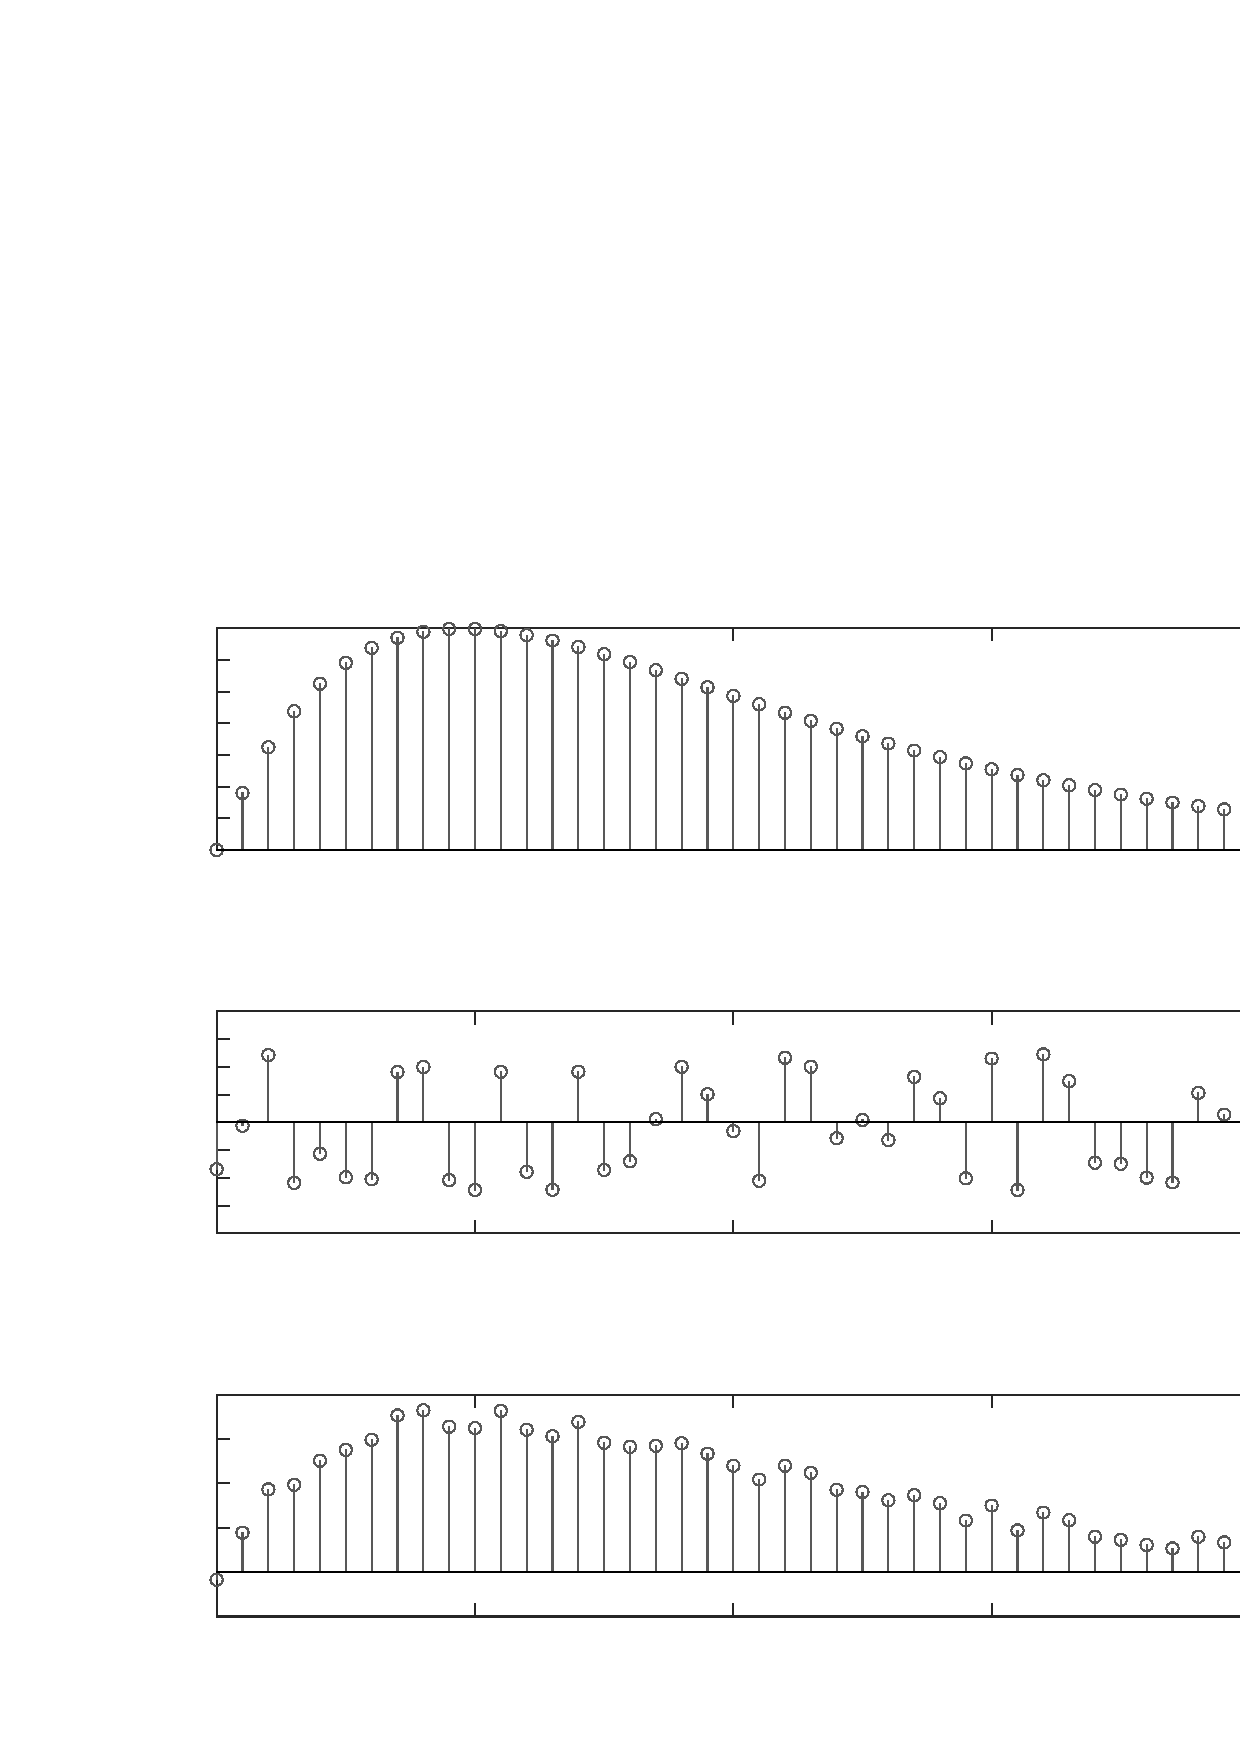
\includegraphics[scale=1]{octaves/ensembleAveraging-inc}
\end{picture}%
\begin{picture}(800,600)(0,0)
\fontsize{13}{0}\selectfont\put(104,423.523){\makebox(0,0)[t]{\textcolor[rgb]{0.15,0.15,0.15}{{0}}}}
\fontsize{13}{0}\selectfont\put(228,423.523){\makebox(0,0)[t]{\textcolor[rgb]{0.15,0.15,0.15}{{10}}}}
\fontsize{13}{0}\selectfont\put(352,423.523){\makebox(0,0)[t]{\textcolor[rgb]{0.15,0.15,0.15}{{20}}}}
\fontsize{13}{0}\selectfont\put(476,423.523){\makebox(0,0)[t]{\textcolor[rgb]{0.15,0.15,0.15}{{30}}}}
\fontsize{13}{0}\selectfont\put(600,423.523){\makebox(0,0)[t]{\textcolor[rgb]{0.15,0.15,0.15}{{40}}}}
\fontsize{13}{0}\selectfont\put(724,423.523){\makebox(0,0)[t]{\textcolor[rgb]{0.15,0.15,0.15}{{50}}}}
\fontsize{13}{0}\selectfont\put(97.0525,433.898){\makebox(0,0)[r]{\textcolor[rgb]{0.15,0.15,0.15}{{0}}}}
\fontsize{13}{0}\selectfont\put(97.0525,449.116){\makebox(0,0)[r]{\textcolor[rgb]{0.15,0.15,0.15}{{1}}}}
\fontsize{13}{0}\selectfont\put(97.0525,464.334){\makebox(0,0)[r]{\textcolor[rgb]{0.15,0.15,0.15}{{2}}}}
\fontsize{13}{0}\selectfont\put(97.0525,479.552){\makebox(0,0)[r]{\textcolor[rgb]{0.15,0.15,0.15}{{3}}}}
\fontsize{13}{0}\selectfont\put(97.0525,494.77){\makebox(0,0)[r]{\textcolor[rgb]{0.15,0.15,0.15}{{4}}}}
\fontsize{13}{0}\selectfont\put(97.0525,509.988){\makebox(0,0)[r]{\textcolor[rgb]{0.15,0.15,0.15}{{5}}}}
\fontsize{13}{0}\selectfont\put(97.0525,525.206){\makebox(0,0)[r]{\textcolor[rgb]{0.15,0.15,0.15}{{6}}}}
\fontsize{13}{0}\selectfont\put(97.0525,540.424){\makebox(0,0)[r]{\textcolor[rgb]{0.15,0.15,0.15}{{7}}}}
\fontsize{15}{0}\selectfont\put(414,550.424){\makebox(0,0)[b]{\textcolor[rgb]{0,0,0}{{Original uncorrupted sequence}}}}
\fontsize{15}{0}\selectfont\put(84.0526,487.161){\rotatebox{90}{\makebox(0,0)[b]{\textcolor[rgb]{0.15,0.15,0.15}{{Amplitude}}}}}
\fontsize{15}{0}\selectfont\put(414,407.523){\makebox(0,0)[t]{\textcolor[rgb]{0.15,0.15,0.15}{{Time index n}}}}
\fontsize{13}{0}\selectfont\put(104,239.574){\makebox(0,0)[t]{\textcolor[rgb]{0.15,0.15,0.15}{{0}}}}
\fontsize{13}{0}\selectfont\put(228,239.574){\makebox(0,0)[t]{\textcolor[rgb]{0.15,0.15,0.15}{{10}}}}
\fontsize{13}{0}\selectfont\put(352,239.574){\makebox(0,0)[t]{\textcolor[rgb]{0.15,0.15,0.15}{{20}}}}
\fontsize{13}{0}\selectfont\put(476,239.574){\makebox(0,0)[t]{\textcolor[rgb]{0.15,0.15,0.15}{{30}}}}
\fontsize{13}{0}\selectfont\put(600,239.574){\makebox(0,0)[t]{\textcolor[rgb]{0.15,0.15,0.15}{{40}}}}
\fontsize{13}{0}\selectfont\put(724,239.574){\makebox(0,0)[t]{\textcolor[rgb]{0.15,0.15,0.15}{{50}}}}
\fontsize{13}{0}\selectfont\put(97.0525,249.949){\makebox(0,0)[r]{\textcolor[rgb]{0.15,0.15,0.15}{{-0.8}}}}
\fontsize{13}{0}\selectfont\put(97.0525,263.265){\makebox(0,0)[r]{\textcolor[rgb]{0.15,0.15,0.15}{{-0.6}}}}
\fontsize{13}{0}\selectfont\put(97.0525,276.58){\makebox(0,0)[r]{\textcolor[rgb]{0.15,0.15,0.15}{{-0.4}}}}
\fontsize{13}{0}\selectfont\put(97.0525,289.896){\makebox(0,0)[r]{\textcolor[rgb]{0.15,0.15,0.15}{{-0.2}}}}
\fontsize{13}{0}\selectfont\put(97.0525,303.212){\makebox(0,0)[r]{\textcolor[rgb]{0.15,0.15,0.15}{{0}}}}
\fontsize{13}{0}\selectfont\put(97.0525,316.527){\makebox(0,0)[r]{\textcolor[rgb]{0.15,0.15,0.15}{{0.2}}}}
\fontsize{13}{0}\selectfont\put(97.0525,329.843){\makebox(0,0)[r]{\textcolor[rgb]{0.15,0.15,0.15}{{0.4}}}}
\fontsize{13}{0}\selectfont\put(97.0525,343.159){\makebox(0,0)[r]{\textcolor[rgb]{0.15,0.15,0.15}{{0.6}}}}
\fontsize{13}{0}\selectfont\put(97.0525,356.475){\makebox(0,0)[r]{\textcolor[rgb]{0.15,0.15,0.15}{{0.8}}}}
\fontsize{15}{0}\selectfont\put(414,366.475){\makebox(0,0)[b]{\textcolor[rgb]{0,0,0}{{Noise}}}}
\fontsize{15}{0}\selectfont\put(68.0525,303.212){\rotatebox{90}{\makebox(0,0)[b]{\textcolor[rgb]{0.15,0.15,0.15}{{Amplitude}}}}}
\fontsize{15}{0}\selectfont\put(414,223.574){\makebox(0,0)[t]{\textcolor[rgb]{0.15,0.15,0.15}{{Time index n}}}}
\fontsize{13}{0}\selectfont\put(104,55.625){\makebox(0,0)[t]{\textcolor[rgb]{0.15,0.15,0.15}{{0}}}}
\fontsize{13}{0}\selectfont\put(228,55.625){\makebox(0,0)[t]{\textcolor[rgb]{0.15,0.15,0.15}{{10}}}}
\fontsize{13}{0}\selectfont\put(352,55.625){\makebox(0,0)[t]{\textcolor[rgb]{0.15,0.15,0.15}{{20}}}}
\fontsize{13}{0}\selectfont\put(476,55.625){\makebox(0,0)[t]{\textcolor[rgb]{0.15,0.15,0.15}{{30}}}}
\fontsize{13}{0}\selectfont\put(600,55.625){\makebox(0,0)[t]{\textcolor[rgb]{0.15,0.15,0.15}{{40}}}}
\fontsize{13}{0}\selectfont\put(724,55.625){\makebox(0,0)[t]{\textcolor[rgb]{0.15,0.15,0.15}{{50}}}}
\fontsize{13}{0}\selectfont\put(97.0525,66){\makebox(0,0)[r]{\textcolor[rgb]{0.15,0.15,0.15}{{-2}}}}
\fontsize{13}{0}\selectfont\put(97.0525,87.3051){\makebox(0,0)[r]{\textcolor[rgb]{0.15,0.15,0.15}{{0}}}}
\fontsize{13}{0}\selectfont\put(97.0525,108.61){\makebox(0,0)[r]{\textcolor[rgb]{0.15,0.15,0.15}{{2}}}}
\fontsize{13}{0}\selectfont\put(97.0525,129.915){\makebox(0,0)[r]{\textcolor[rgb]{0.15,0.15,0.15}{{4}}}}
\fontsize{13}{0}\selectfont\put(97.0525,151.22){\makebox(0,0)[r]{\textcolor[rgb]{0.15,0.15,0.15}{{6}}}}
\fontsize{13}{0}\selectfont\put(97.0525,172.525){\makebox(0,0)[r]{\textcolor[rgb]{0.15,0.15,0.15}{{8}}}}
\fontsize{15}{0}\selectfont\put(414,182.525){\makebox(0,0)[b]{\textcolor[rgb]{0,0,0}{{Corrupted sequence}}}}
\fontsize{15}{0}\selectfont\put(79.0526,119.263){\rotatebox{90}{\makebox(0,0)[b]{\textcolor[rgb]{0.15,0.15,0.15}{{Amplitude}}}}}
\fontsize{15}{0}\selectfont\put(414,39.6249){\makebox(0,0)[t]{\textcolor[rgb]{0.15,0.15,0.15}{{Time index n}}}}
\end{picture}

% Title: gl2ps_renderer figure
% Creator: GL2PS 1.4.2, (C) 1999-2020 C. Geuzaine
% For: Octave
% CreationDate: Wed Oct 19 09:02:39 2022
\setlength{\unitlength}{1pt}
\begin{picture}(0,0)
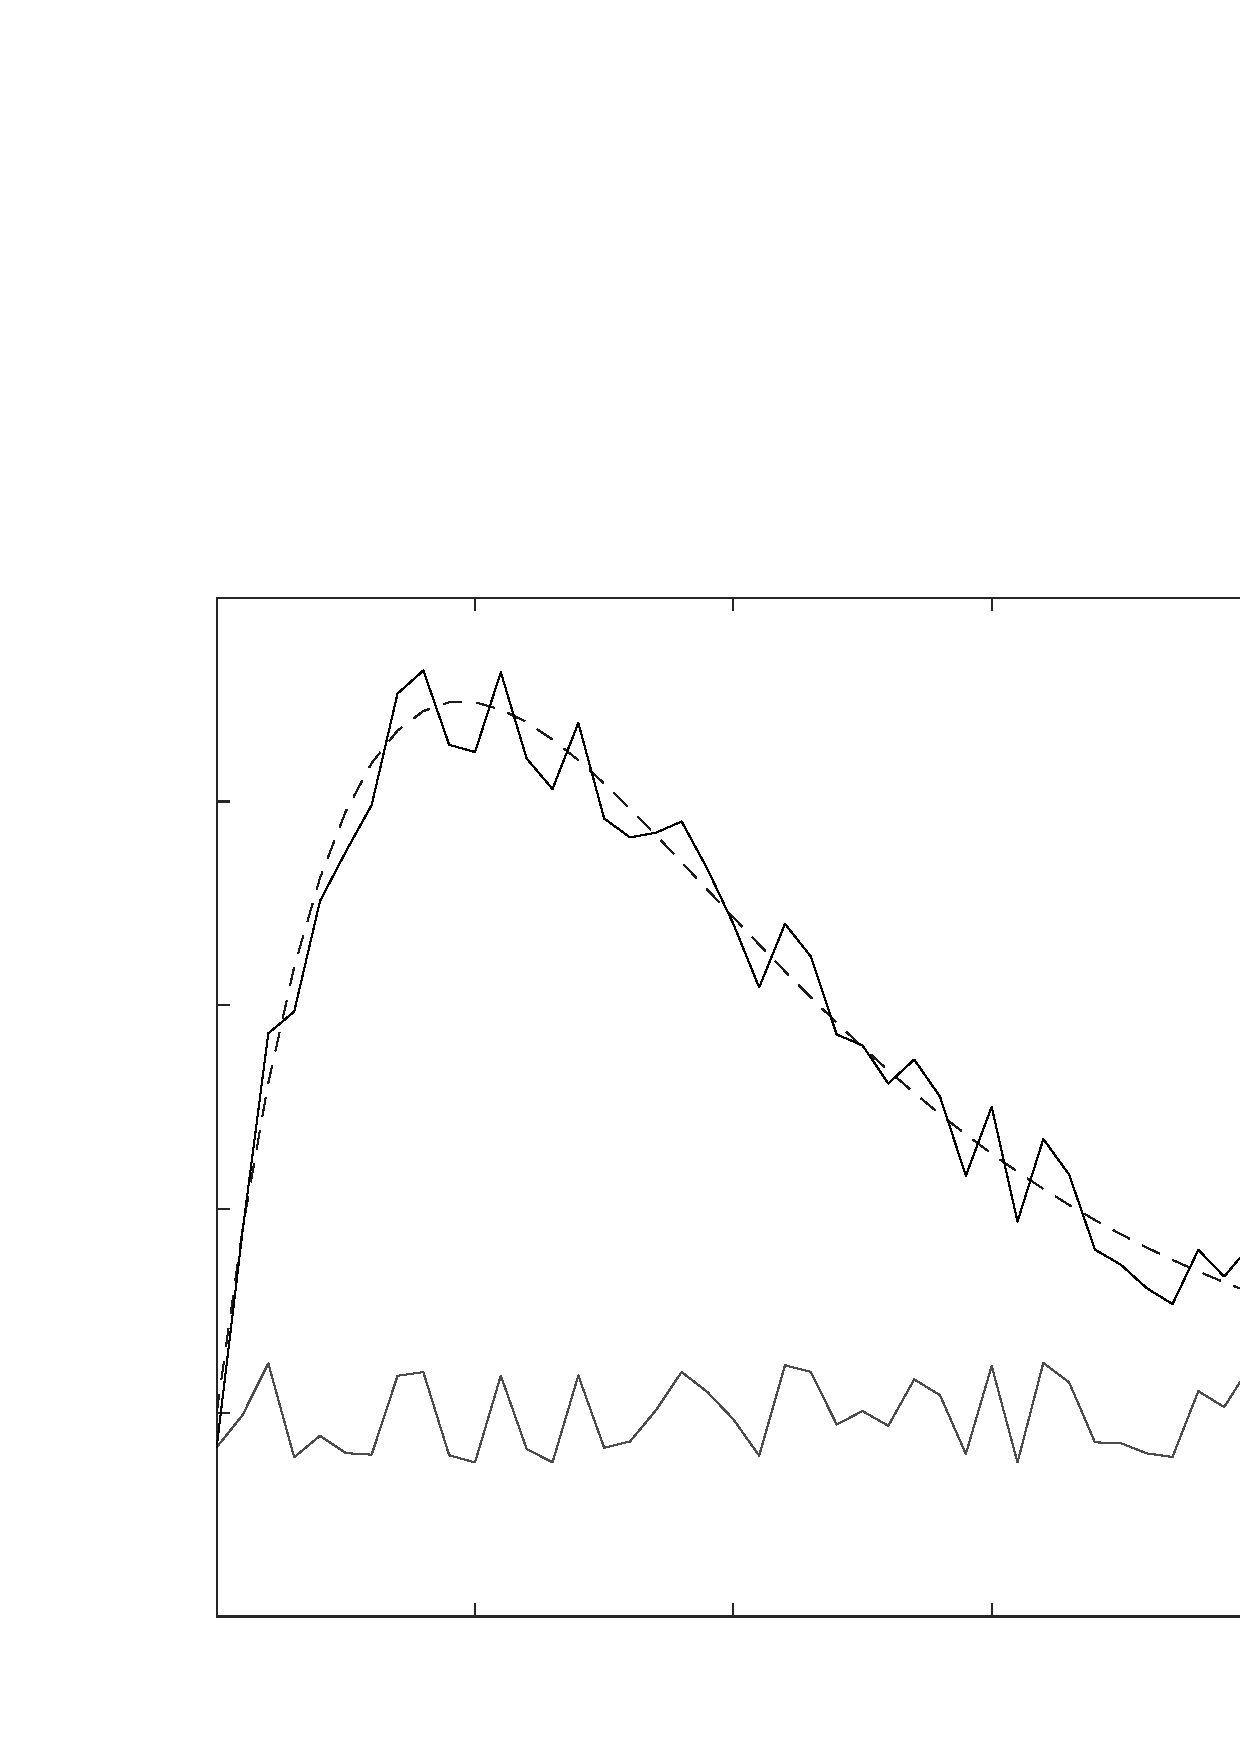
\includegraphics[scale=1]{octaves/ensembleAveragingTwo-inc}
\end{picture}%
\begin{picture}(800,600)(0,0)
\fontsize{13}{0}\selectfont\put(104,55.5788){\makebox(0,0)[t]{\textcolor[rgb]{0.15,0.15,0.15}{{0}}}}
\fontsize{13}{0}\selectfont\put(228,55.5788){\makebox(0,0)[t]{\textcolor[rgb]{0.15,0.15,0.15}{{10}}}}
\fontsize{13}{0}\selectfont\put(352,55.5788){\makebox(0,0)[t]{\textcolor[rgb]{0.15,0.15,0.15}{{20}}}}
\fontsize{13}{0}\selectfont\put(476,55.5788){\makebox(0,0)[t]{\textcolor[rgb]{0.15,0.15,0.15}{{30}}}}
\fontsize{13}{0}\selectfont\put(600,55.5788){\makebox(0,0)[t]{\textcolor[rgb]{0.15,0.15,0.15}{{40}}}}
\fontsize{13}{0}\selectfont\put(724,55.5788){\makebox(0,0)[t]{\textcolor[rgb]{0.15,0.15,0.15}{{50}}}}
\fontsize{13}{0}\selectfont\put(97.0525,66){\makebox(0,0)[r]{\textcolor[rgb]{0.15,0.15,0.15}{{-2}}}}
\fontsize{13}{0}\selectfont\put(97.0525,163.8){\makebox(0,0)[r]{\textcolor[rgb]{0.15,0.15,0.15}{{0}}}}
\fontsize{13}{0}\selectfont\put(97.0525,261.6){\makebox(0,0)[r]{\textcolor[rgb]{0.15,0.15,0.15}{{2}}}}
\fontsize{13}{0}\selectfont\put(97.0525,359.4){\makebox(0,0)[r]{\textcolor[rgb]{0.15,0.15,0.15}{{4}}}}
\fontsize{13}{0}\selectfont\put(97.0525,457.2){\makebox(0,0)[r]{\textcolor[rgb]{0.15,0.15,0.15}{{6}}}}
\fontsize{13}{0}\selectfont\put(97.0525,555){\makebox(0,0)[r]{\textcolor[rgb]{0.15,0.15,0.15}{{8}}}}
\fontsize{15}{0}\selectfont\put(414,39.5788){\makebox(0,0)[t]{\textcolor[rgb]{0.15,0.15,0.15}{{Time index n}}}}
\fontsize{15}{0}\selectfont\put(79.0526,310.5){\rotatebox{90}{\makebox(0,0)[b]{\textcolor[rgb]{0.15,0.15,0.15}{{Amplitude}}}}}
\fontsize{12}{0}\selectfont\put(693.005,536.005){\makebox(0,0)[l]{\textcolor[rgb]{0,0,0}{{x[n]}}}}
\fontsize{12}{0}\selectfont\put(693.005,518.007){\makebox(0,0)[l]{\textcolor[rgb]{0,0,0}{{y[n]}}}}
\end{picture}

}\caption{The ensemble averaging. On the left, the original uncorrupted sequence $s[n]$, the noise $d[n]$ and the corrupted sequence $x[n]$. On the right, the dashed line represents the sequence $y[n]$, a ``recovered'' version of the original sequence $s[n]$. Recovering has been performed by means of the ensemble averaging process.}\label{oct:ensembleAveraging}
\end{center}
\end{figure*}

\section{Sample Rate Alteration}

The operation of alterating the sample rate $F_S$ is much important. Generally, it is adopted to obtain a new signal $x'$ from a signal $x$, but with a different sample rate $F'_S$. The new sample rate can either be high\-er or lower than the original signal, so that a \emph{sampling rate alteration ratio} can be defined,
\begin{equation}\label{eqn:SamplingRateAlterationRatio}
	R_S = \frac{F'_S}{F_S}.
\end{equation}

The ratio in equation \ref{eqn:SamplingRateAlterationRatio} can either be greater or lower than $1$, and determines the nature of the sample rate alteration. In particolar, in the case of $R_S > 1$ one performs the \textbf{interpolation} operation, while in the opposite case of $R_S < 1$ one gets the \textbf{decimation} operation. 

Two operations are necessary for, respectively, interpolation and decimation: the \emph{up-sampling} and the \emph{down-sam\-pling} operations. To be specific, in order to perform interpolation a \emph{further} operation is needed other than up-sampling.

\subsubsection{Up-Sampling}

The up-sampling operation by an integer factor $L > 1$ involves the addition of
$L-1$ zero-valued samples inserted between two consecutive samples of the
original signal:

\begin{equation}\label{eqn:UpSampling}
	x_u[n] =
	\left\{
		\begin{array}{ll}
			x[n/L] 	& n=0,\pm L, \pm 2L, \dots \\
			0 	& otherwise
		\end{array}
	\right.
\end{equation}

Up-sampling operation is denoted by a $\uparrow L$ block, as in Diagram~\ref{tikz:upsamplingOperation}. Upsampling is usually followed by \emph{interpolation}. 

\begin{figure}[ht]
\begin{center}
    \begin{tikzpicture}
    \node [](A){$x[n]$};
    \node [draw,rectangle,thick](B) at (1.5,0){$\uparrow L$}; 
    \node [](C) at(3,0){$x_u[n]$}; 
    \draw[->] (A) -- (B) -- (C);
\end{tikzpicture}\caption{Notation for the up-sampling operation by a factor $L$.}\label{tikz:upsamplingOperation}
\end{center}
\end{figure}

\subsubsection{Down-Sampling}

The down-sampling operation by an integer factor $M > 1$ means that from the
original signal only one sample every $M$ is preserved. This way, $M-1$ consecutive
in-between samples are removed from the signal, while a single one every $M$ samples is preserved,
\begin{equation}\label{eqn:DownSampling}
	x_d[n] = x[nM]
\end{equation}

Down-sampling operation is denoted by a $\downarrow M$ block, as in Figure~\ref{tikz:downsamplingOperation}.
\begin{figure}[ht]
\begin{center}
    \begin{tikzpicture}
    \node [](A){$x[n]$};
    \node [draw,rectangle,thick](B) at (1.5,0){$\downarrow M$}; 
    \node [](C) at(3,0){$x_u[n]$}; 
    \draw[->] (A) -- (B) -- (C);
\end{tikzpicture}\caption{Notation for the down-sampling operation by a factor $M$.}\label{tikz:downsamplingOperation}
\end{center}
\end{figure}
The result of downsampling is a se\-quen\-ce in which some values are missing, those that are removed by the downsampling operation. A crucial risk of downsampling that we will tackle is the \textbf{aliasing} phenomenon.
\begin{figure*}[ht]
    \centering
    \scalebox{0.6}{
    % Title: gl2ps_renderer figure
% Creator: GL2PS 1.4.2, (C) 1999-2020 C. Geuzaine
% For: Octave
% CreationDate: Wed Oct 19 09:18:32 2022
\setlength{\unitlength}{1pt}
\begin{picture}(0,0)
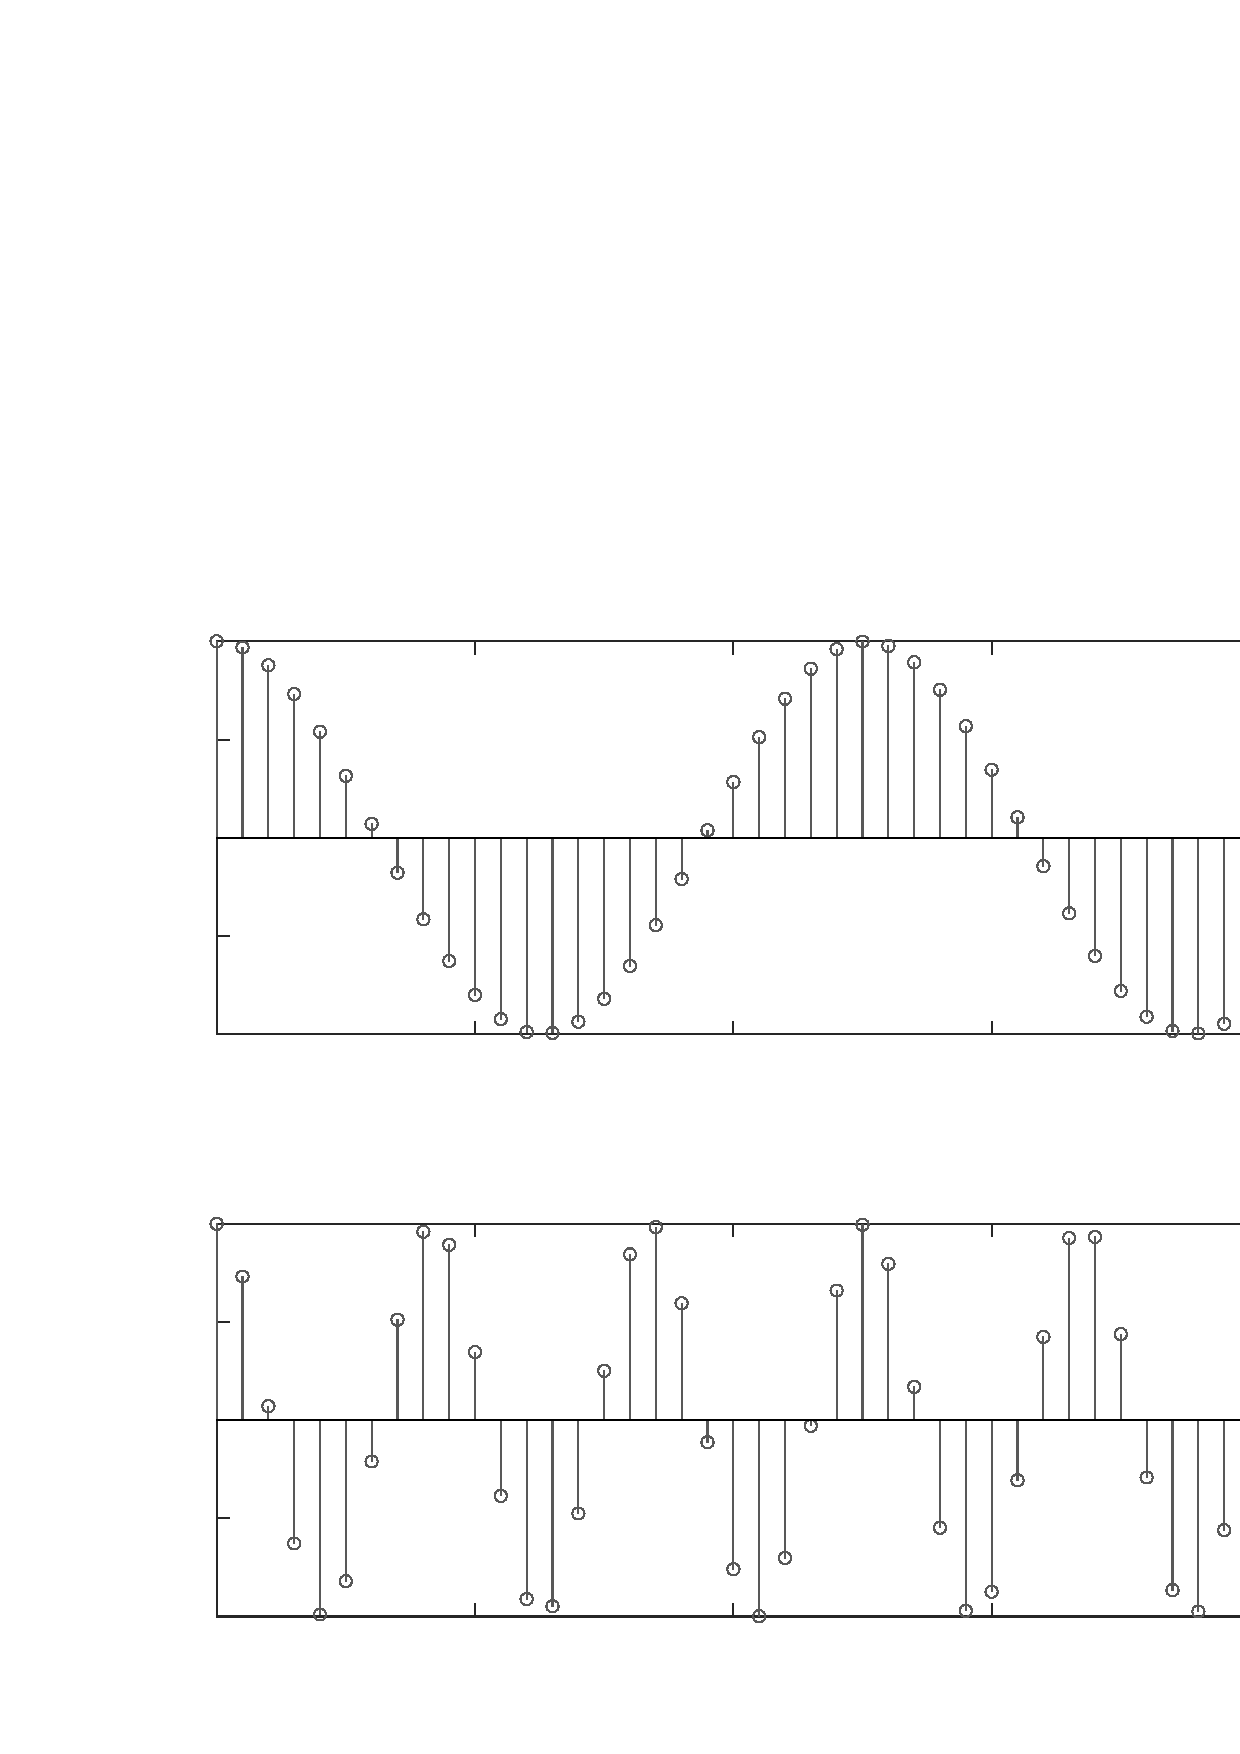
\includegraphics[scale=1]{octaves/downsamplingOperationEffect-inc}
\end{picture}%
\begin{picture}(800,600)(0,0)
\fontsize{13}{0}\selectfont\put(104,335.117){\makebox(0,0)[t]{\textcolor[rgb]{0.15,0.15,0.15}{{0}}}}
\fontsize{13}{0}\selectfont\put(228,335.117){\makebox(0,0)[t]{\textcolor[rgb]{0.15,0.15,0.15}{{10}}}}
\fontsize{13}{0}\selectfont\put(352,335.117){\makebox(0,0)[t]{\textcolor[rgb]{0.15,0.15,0.15}{{20}}}}
\fontsize{13}{0}\selectfont\put(476,335.117){\makebox(0,0)[t]{\textcolor[rgb]{0.15,0.15,0.15}{{30}}}}
\fontsize{13}{0}\selectfont\put(600,335.117){\makebox(0,0)[t]{\textcolor[rgb]{0.15,0.15,0.15}{{40}}}}
\fontsize{13}{0}\selectfont\put(724,335.117){\makebox(0,0)[t]{\textcolor[rgb]{0.15,0.15,0.15}{{50}}}}
\fontsize{13}{0}\selectfont\put(97.0525,345.566){\makebox(0,0)[r]{\textcolor[rgb]{0.15,0.15,0.15}{{-1}}}}
\fontsize{13}{0}\selectfont\put(97.0525,392.691){\makebox(0,0)[r]{\textcolor[rgb]{0.15,0.15,0.15}{{-0.5}}}}
\fontsize{13}{0}\selectfont\put(97.0525,439.816){\makebox(0,0)[r]{\textcolor[rgb]{0.15,0.15,0.15}{{0}}}}
\fontsize{13}{0}\selectfont\put(97.0525,486.941){\makebox(0,0)[r]{\textcolor[rgb]{0.15,0.15,0.15}{{0.5}}}}
\fontsize{13}{0}\selectfont\put(97.0525,534.066){\makebox(0,0)[r]{\textcolor[rgb]{0.15,0.15,0.15}{{1}}}}
\fontsize{15}{0}\selectfont\put(414,544.066){\makebox(0,0)[b]{\textcolor[rgb]{0,0,0}{{Original sequence}}}}
\fontsize{13}{0}\selectfont\put(104,55.6063){\makebox(0,0)[t]{\textcolor[rgb]{0.15,0.15,0.15}{{0}}}}
\fontsize{13}{0}\selectfont\put(228,55.6063){\makebox(0,0)[t]{\textcolor[rgb]{0.15,0.15,0.15}{{10}}}}
\fontsize{13}{0}\selectfont\put(352,55.6063){\makebox(0,0)[t]{\textcolor[rgb]{0.15,0.15,0.15}{{20}}}}
\fontsize{13}{0}\selectfont\put(476,55.6063){\makebox(0,0)[t]{\textcolor[rgb]{0.15,0.15,0.15}{{30}}}}
\fontsize{13}{0}\selectfont\put(600,55.6063){\makebox(0,0)[t]{\textcolor[rgb]{0.15,0.15,0.15}{{40}}}}
\fontsize{13}{0}\selectfont\put(724,55.6063){\makebox(0,0)[t]{\textcolor[rgb]{0.15,0.15,0.15}{{50}}}}
\fontsize{13}{0}\selectfont\put(97.0525,66){\makebox(0,0)[r]{\textcolor[rgb]{0.15,0.15,0.15}{{-1}}}}
\fontsize{13}{0}\selectfont\put(97.0525,113.125){\makebox(0,0)[r]{\textcolor[rgb]{0.15,0.15,0.15}{{-0.5}}}}
\fontsize{13}{0}\selectfont\put(97.0525,160.25){\makebox(0,0)[r]{\textcolor[rgb]{0.15,0.15,0.15}{{0}}}}
\fontsize{13}{0}\selectfont\put(97.0525,207.375){\makebox(0,0)[r]{\textcolor[rgb]{0.15,0.15,0.15}{{0.5}}}}
\fontsize{13}{0}\selectfont\put(97.0525,254.5){\makebox(0,0)[r]{\textcolor[rgb]{0.15,0.15,0.15}{{1}}}}
\fontsize{15}{0}\selectfont\put(414,264.5){\makebox(0,0)[b]{\textcolor[rgb]{0,0,0}{{Downsampled sequence by a factor of 3}}}}
\end{picture}

    }\caption{Example of down-sampling operation applied to a sinusoidal input se\-quen\-ce.}\label{oct:downsamplingOperationEffect}
\end{figure*}


\section{Classification of se\-quen\-ces}

There are several ways to classify a se\-quen\-ce.

The first one is by \textbf{symmetry}. A \emph{conjugate-symmetric} se\-quen\-ce is a se\-quen\-ce that satisfies the property \[x[n] = x^*[-n];\] If $x$ is real, then it is said to be an \emph{even se\-quen\-ce}. The \emph{conjugate antisymetric se\-quen\-ce}, on contrary, is such that \[x[n] = -x^*[-n],\] and if $x$ is real, then it is said to be an \emph{odd se\-quen\-ce}. Every se\-quen\-ce can be defined with the sum of its conjugate symmetric and antisimetric parts\footnote{In fact, $x_{cs} = \frac{1}{2}(x[n] + x^*[-n])$ and $x_{as} = \frac{1}{2}(x[n] - x^*[-n])$.}, that are two distinct signals \[x[n] = x_{cs}[n] + x_{ca}[n];\]

Another way is by \textbf{periodicity}: a se\-quen\-ce $\tilde{x}[n]$ is \emph{periodic with period} $N$ if it satisfies the property \[\tilde{x}[n] = \tilde{x}[n + kN]\] for some $N \in \Z$. Smallest $N$ value that satisfies such property is called \emph{fundamental period}. A se\-quen\-ce that does not satisfy this property is said to be \emph{aperiodic}. The sum of two periodic signals $x_a$ and $x_b$ of fundamental period---respectively---$N_a$ and $N_b$ is still a periodic se\-quen\-ce, having fundamental period $N_f$ of \[N_f = \frac{N_a N_b}{\mathrm{GCD}(N_a, N_b)} \geq \max{(N_a, N_b)},\] where $\mathrm{GCD}$ is the ``greatest common divisor'' operation;

One can also compute the \textbf{total energy} of a signal $x$, defined as the quantity 
\begin{equation}\label{eqn:totalEnergy}
    \mathcal E_x = \sum_{n=-\infty}^{\infty} | x[n] |^2.
\end{equation}
A finite-length se\-quen\-ce will possess finite energy, but an infinite-length se\-quen\-ce might have finite or infinite energy depending on the nature of the signal. Among with the definition of energy, it comes the definition of \textbf{average power} of a signal, which is, specifically,
\begin{equation}\label{eqn:averagePower}
    P_x = \lim_{K \rightarrow \infty} \frac{1}{2K + 1} \sum_{n = -K}^K |x[n]|^2.
\end{equation}
The average power formula may depend on the nature of the signal. In particular, 
\begin{itemize}
    \item regarding \emph{aperiodic} signals, the average power is
        \[ P_x = \lim_{K \rightarrow \infty} \frac{1}{2K + 1} \sum_{n = -K}^K |x[n]|^2, \]
    and---recalling the definition of total energy---can thus be rewritten as
    \[ P_x = \lim_{K \rightarrow \infty} \frac{1}{2K + 1} \mathcal E_{x,K}; \]
    \item regarding \emph{periodic} signals with period $N$, the average power is
        \[P_x = \frac{1}{N} \sum_{n = 0}^{N-1} |x[n]|^2,\] a quantity that is computed through a period and might be finite or infinite\footnote{To introduce some examples, consider a causal se\-quen\-ce defined by \[ x[n] = \left\{\begin{array}{lc}3(-1)^n, & n \geq 0\\ 0, & n < 0\end{array}\right. .\] se\-quen\-ce $x$ has infinite energy. The average power is given by \[P_x = \lim_{K\rightarrow \infty}\frac{1}{2K+1}\left(9\sum_{n=0}^K 1\right) = \lim_{K\rightarrow \infty}\frac{9(K+1)}{2K+1} = 4.5,\] a finite quantity, of course.}. A periodic se\-quen\-ce that possesses an infinite energy---but finite average power---is said to be a \emph{power signal}. Instead, a finite energy signal with infinite length possessing zero average power is said to be an \emph{energy signal}. Energy signals and power signals are peculiar se\-quen\-ces that satisfy some specific properties.
\end{itemize}
A se\-quen\-ce $x[n]$ is said to be \textbf{bounded} if \[|x[n]| \leq B_x < \infty,\] when the greatest value---in absolute value---of the se\-quen\-ce is smaller than a certain \emph{bound} $B_x$ of the se\-quen\-ce $x$. The se\-quen\-ce $x[n] = \cos{0.3\pi n}$ is a bounded se\-quen\-ce since \[|x[n]| = |\cos{0.3\pi n}| \leq 1.\]

A se\-quen\-ce is \textbf{absolutely summable} if the sum of all its absolute values for all of its samples samples is a limited quantity\footnote{For example, se\-quen\-ce \[y[n] = \left\{\begin{array}{lc} 0.3^n, & n \geq 0 \\ 0, & n < 0\end{array}\right.\] is absolutely summable since \[ \sum_{n=0}^\infty |0.3^n| = \frac{1}{1 - 0.3} < \infty.\]}  An absolutely summable sequence is a sequence such that 
\begin{equation}\label{eqn:absolutelySummableSequence}
    \sum_{n=-\infty}^{\infty}|x[n]| < \infty.
\end{equation} 
As we will see later, absolute summability implies that the Fourier transform converges uniformly, so this means that the unit circle is contained in the region of convergence (ROC).

At last, a se\-quen\-ce $x[n]$ is \textbf{square-summable} if  \[\sum_{n=-\infty}^{\infty}|x[n]|^2 < \infty,\] in a similar fashion to the absolutely summable case. se\-quen\-ces can be absolutely summable but not squa\-re-sum\-ma\-ble, and the contrary can occur as well. For instance, if one considers the se\-quen\-ce $k[n] = \frac{\sin{0.4n}}{\pi n}$ will find out that it is squa\-re-sum\-ma\-ble but \textbf{not} absolutely summable.

\section{Basic se\-quen\-ces}
Basic se\-quen\-ces are the fundamental se\-quen\-ces that will be encountered throughout the study of signals.
There are several kinds of notable basic se\-quen\-ces. All of them possess peculiar properties which are paramount to the discipline of signal theory.

The first one to be mentioned is the \textbf{unit sample se\-quen\-ce}, also called the \textbf{impulse se\-quen\-ce}. It is a special signal whose only sample different from zero is the sample in the origin: \[\delta[n] = \left\{\begin{array}{ll} 1 & n = 0\\ 0 & n \neq 0 \end{array}\right..\]

\begin{center}
\begin{tikzpicture}
    %\node[above,font=\bfseries] at (0,3.5) {The unit sample se\-quen\-ce};
    \draw[->] (-3.2,0) -- (3.2,0) node[anchor=north west] {$t$};
    \draw[->] (0,0) -- (0,2.5) node[anchor=south east] {$\delta$};
    \draw[thick] (0,0) -- (0,2);

\foreach \x in {-3,-2,-1,0,1,2,3}
    \draw (\x cm,1pt) -- (\x cm,-1pt) node[anchor=north] {$\x$};

    \draw (1 pt,2cm) -- (-1 pt,2cm) node[anchor=north east] {$1$};
    \node [draw,inner sep=1pt, circle, thick](A) at (-3,0){};
    \node [draw,inner sep=1pt, circle, thick](B) at (-2,0){};
    \node [draw,inner sep=1pt, circle, thick](C) at (-1,0){};
    \node [draw,inner sep=1pt, circle, thick](D) at (0,2){};
    \node [draw,inner sep=1pt, circle, thick](E) at (1,0){};
    \node [draw,inner sep=1pt, circle, thick](F) at (2,0){};
    \node [draw,inner sep=1pt, circle, thick](G) at (3,0){};
\end{tikzpicture}
\end{center}

In practice, the ``delta impulse'' can be used to show a lot of interesting properties, and it is indeed the kernel of the convolution filter.

Let's continue with the second basic se\-quen\-ce.

Defined as \[\mu[n] = \left\{\begin{array}{ll}1, & n \geq 0 \\ 0, & n < 0\end{array}\right.,\] the \textbf{unit step se\-quen\-ce} is the integral of the impulse se\-quen\-ce. Indeed, when summing up all the values of the unit impulse se\-quen\-ce one has only $0$s until the only non-zero value occurs and the value of the integral collapses to the unit $1$.

\begin{center}
\begin{tikzpicture}
    %\node[above,font=\large\bfseries] at (0,3.5) {Unit sample se\-quen\-ce};
    \draw[->] (-3.2,0) -- (3.2,0) node[anchor=north west] {$t$};
    \draw[->] (0,0) -- (0,2.5) node[anchor=south east] {$\mu$};
    \draw[thick] (0,0) -- (0,2);
    \draw[thick] (1,0) -- (1,2);
    \draw[thick] (2,0) -- (2,2);
    \draw[thick] (3,0) -- (3,2);

\foreach \x in {-3,-2,-1,0,1,2,3}
    \draw (\x cm,1pt) -- (\x cm,-1pt) node[anchor=north] {$\x$};

    \draw (1 pt,2cm) -- (-1 pt,2cm) node[anchor=north east] {$1$};
    \node [draw,inner sep=1pt, circle, thick](A) at (-3,0){};
    \node [draw,inner sep=1pt, circle, thick](B) at (-2,0){};
    \node [draw,inner sep=1pt, circle, thick](C) at (-1,0){};
    \node [draw,inner sep=1pt, circle, thick](D) at (0,2){};
    \node [draw,inner sep=1pt, circle, thick](E) at (1,2){};
    \node [draw,inner sep=1pt, circle, thick](F) at (2,2){};
    \node [draw,inner sep=1pt, circle, thick](G) at (3,2){};
\end{tikzpicture}
\end{center}

A \textbf{real sinusoidal se\-quen\-ce} is a se\-quen\-ce defined as \[x[n] = A\cos{(\omega_0 n + \varphi)},\] where $A$ is the \emph{amplitude} of the sinusoid, $\omega_0$ is the \emph{angular frequency} and $\varphi$ is the \emph{phase} of $x[n]$. A real sinusoid se\-quen\-ce therefore possesses amplitude, (angular) frequency and phase as intrinsic properties. Sinusoids fulfill an important role as they are signals whose amplitude and frequency stays the same throughout the time and are describable with sine and cosine ``elementary'' functions.

An indeed important family of se\-quen\-ces are the \textbf{exponential se\-quen\-ces}, all of them having form \[x[n] = A\alpha^n, -\infty < n < \infty,\] where $A, \alpha \in \C$ can be either real or complex numbers. The various kinds of exponentials arise from peculiar choices of coefficient and basis, as the behavior will dramatically change depending on the nature of both.

In general, an exponential se\-quen\-ce can be expressed expanding modulus and phase of both numbers, obtaining \[x[n] = |A|e^{j\varphi}e^{(\sigma_0 + j\omega_0)n} = x_{re}[n] + jx_{im}[n]\] a partitioning into real and imaginary part of the se\-quen\-ce. In particular, one has 
\begin{align} 
    x_{re}[n] & = |A|e^{\sigma_0n}\cos{(\omega_0 n + \varphi)},\\
    x_{im}[n] & = |A|e^{\sigma_0n}\sin{(\omega_0 n + \varphi)}.
\end{align}

Following this idea, the analysis of both terms indicate two different behaviors depending on the nature of $A$ and $\alpha$. Suppose $A \in \C$ and $\alpha \in \C$. The first and second terms---related to the real and imaginary parts of the exponential se\-quen\-ce---are two real, sinusoidal se\-quen\-ces with constant ($\sigma_0 = 0$), growing ($\sigma_0 > 0$) or decaying ($\sigma_0 < 0$) amplitudes for samples $n > 0$. In practice, they are sinusoids whose angular frequency and phase are determined, respectively, by terms $\omega_0$ and $\varphi$, and whose amplitude varies according to the term $e^{\sigma_0n}$ with the exception of a multiplication constant $|A|$, the modulus of the complex number $A \in \C$. Still, their value at zero will be different as they are described by either sine or cosine, but the overall behavior will be the same: either decaying, or growing, or they are sinusoids of constant amplitude.

Let now $A,\alpha \in \R$. Real exponential se\-quen\-ces are the ``classic'' exponential se\-quen\-ces, described by \[x[n] = A\alpha^n\] and possibly constant within the special case $\alpha=1$. In practice,
\begin{itemize}
    \item for values $\alpha < 1$, the exponential will decay;
    \item for values $\alpha > 1$, the exponential will grow over time.
\end{itemize}

Both sinusoidal se\-quen\-ces and complex exponential se\-quen\-ces are periodic se\-quen\-ces of period $N$ if 
\begin{equation}\label{eqn:sinusoidExponentialPeriod}
\omega_0 N = 2\pi r
\end{equation}
holds, with the very same parameters as in the above models and with $r,N \in \N$. As it goes for general periodic signals, the smallest value of $N$ that satisfies the \ref{eqn:sinusoidExponentialPeriod} is the \emph{fundamental period} of the se\-quen\-ce.
\begin{proof}
In order to verify this, two very similar se\-quen\-ces must be picked---the same se\-quen\-ce but original and shifted of $N$ samples:
\begin{align}
    x_1[n] &= \cos{(\omega_0 n + \varphi)},\\
    x_2[n] &= \cos{(\omega_0 (n + N) + \varphi)}.
\end{align}

Now, the second se\-quen\-ce can be soon rewritten as
\begin{align}
    x_2[n] &= \cos{(\omega_0 (n + N) + \varphi)},\\
           &= \cos{(\omega_0 n + \varphi)}\cos{\omega_0 N} - \sin{(\omega_0 n + \varphi)}\sin{\omega_0 N}.\label{eqn:proofSinusoidPeriod}
\end{align}

The \ref{eqn:proofSinusoidPeriod} will be equal to $x_1[n]$ if and only if \begin{equation}\sin{\omega_0 N} = 0 \wedge \cos{\omega_0 N} = 1,\end{equation} two conditions that are met if and only if the \ref{eqn:sinusoidExponentialPeriod} is satisfied. Alternatively, the very same equation---but re\-ar\-ran\-ged---must be satisfied,
\begin{equation}\label{eqn:sinusoidExponentialPeriodFraction}
    \frac{2\pi}{\omega_0} = \frac{N}{r}.
\end{equation}
\end{proof}

Along with this proof, one might say that $N$ is the \emph{true} period, while the quantity $\frac{N}{r}$ is the \emph{apparent} period---the one of the implied continuous function. In fact, if $\frac{2\pi}{\omega_0}$ is a noninteger rational number, then the period will be a multiple of $\frac{2\pi}{\omega_0}$, which basically means $r > 1$. Otherwise, in the case of an irrational $\frac{2\pi}{\omega_0}$ the discrete se\-quen\-ce will be aperiodic.

For instance, if one considers \[x[n] = \sin{(\sqrt{3}n + \varphi)},\] this (discrete) se\-quen\-ce will be aperiodic regardless of the fact that the continuous function would still be a periodic signal. In fact, substituting in \ref{eqn:sinusoidExponentialPeriodFraction} yields \[\frac{2\pi}{\sqrt{3}} = \frac N r,\] resulting in a quantity on the left that can never be rational as the right member of the equation. This is because the \ref{eqn:sinusoidExponentialPeriodFraction} strictly requires that the angular frequency is an irrational number---a multiple of $\pi$, to be accurate---in order to fulfill the condition of rationality.

\subsection{Frequency properties of basic sinusoidal se\-quen\-ces}

Let's now focus on the peculiar properties of sinusoidal and exponential basis se\-quen\-ces.

To begin with, consider se\-quen\-ces $x[n] = \exp{j \omega_1 n}$ and $y[n] = \exp{j \omega_2 n}$, with $0 \leq \omega_1 < \pi$ and $2 \pi k \leq \omega_2 < \pi(2k+1)$, with $k$ positive integer. If $\omega_2 = \omega_1 + 2 \pi k$, then $x[n] \equiv y[n]$: se\-quen\-ces $x$ and $y$ are \emph{indistinguishable} from each other. This means that for (complex) exponential se\-quen\-ces a shift of $2\pi k$ leads to \emph{the very same} se\-quen\-ce, as the resulting shifted se\-quen\-ce will be exactly the same as the original one.

Another paramount property revolves around the oscillation frequency of a sinusoid $x[n]=\cos{(\omega_0 n)}$. In practice, the frequency of oscillation increases as $\omega_0$ goes from $0$ to $\pi$, while the contrary happens when moving from $\pi$ to $2\pi$. What does this mean?

That is a property of \emph{discrete} sinusoids: the frequency of oscillation is the greatest around $\omega=\pi$, while it is the lowest possible for frequencies close to $0$ or close to $2\pi$. The first frequencies are said to be \textbf{high frequencies}, while the latter ones are the \textbf{low frequencies}.

For the first considered property, a sinusoidal se\-quen\-ce having frequency $\omega_0$ in the neighborhood of $\omega=2\pi k$ is indistinguishable from another sinusoidal se\-quen\-ce whose frequency is $\omega_0 - 2 \pi k$, in the neighborhood of $\omega = 0$. Along with the same reasoning, any frequency $\omega_0$ in the neighborhood of $\omega = \pi (2k + 1)$ is indistinguishable from a frequency $\omega_0 - \pi(2k + 1)$ in the neighborhood of $\omega = \pi$.

Actually, what happens is that the oscillation shows a \emph{periodic} behavior across the frequency---hence, it is possible to describe the entire frequency space with the sole range of values $[0, \pi]$, as the other half $[\pi, 2\pi]$ is completely symmetric to the first range.

As previously said, frequencies in neighborhood of $\omega = 2 \pi k$ are the low frequencies, in contrast to those in the neighborhood of $\omega = \pi (2k + 1)$ that are the high frequencies\footnote{The se\-quen\-ce \[v_1[n] = \cos{(0.1 \pi n)} \equiv \cos{(1.9\pi n)}\] is a low frequency signal, while se\-quen\-ce \[v_2[n] = \cos{(0.8 \pi n)} \equiv \cos{(1.2\pi n)}\] is a high frequency one.}.

\subsection{Representation of a se\-quen\-ce with basic se\-quen\-ces}

Any arbitrary se\-quen\-ce can be represented in the time domain as a \emph{weighted sum} of some basic se\-quen\-ces and its delayed--advanced versions.

\begin{center}
\begin{tikzpicture}
    \node[below,font=\bfseries] at (0,-1.5) {$x[n] = 0.8\delta[n+3] -0.9\delta[n+1] + 1.2\delta[n-1] + \delta[n-4]$};
    \draw[->] (-2.7,0) -- (2.7,0) node[anchor=north west] {$n$};
    \draw[thick] (-1.5,0) -- (-1.5,0.8);
    \draw[thick] (-.5,0) -- (-.5,-0.9);
    \draw[thick] (.5,0) -- (.5,1.2);
    \draw[thick] (2,0) -- (2,1);

\foreach \x in {-5,-4,...,5}
    \draw (\x*0.5 cm,1pt) -- (\x*0.5 cm,-1pt) node[anchor=north] {$\x$};

    \node [draw,inner sep=1pt, circle, thick](A) at (-2.5,0){};
    \node [draw,inner sep=1pt, circle, thick](B) at (-2.0,0){};
    \node [draw,inner sep=1pt, circle, thick,label=right:{$0.8$}](C) at (-1.5,0.8){};
    \node [draw,inner sep=1pt, circle, thick](D) at (-1.0,0){};
    \node [draw,inner sep=1pt, circle, thick,label=right:{$-0.9$}](E) at (-.5,-0.9){};
    \node [draw,inner sep=1pt, circle, thick](F) at (0,0){};
    \node [draw,inner sep=1pt, circle, thick,label=right:{$1.2$}](G) at (.5,+1.2){};
    \node [draw,inner sep=1pt, circle, thick](H) at (1,0){};
    \node [draw,inner sep=1pt, circle, thick](I) at (1.5,0){};
    \node [draw,inner sep=1pt, circle, thick,label=right:{$1$}](J) at (2,1){};
    \node [draw,inner sep=1pt, circle, thick](K) at (2.5,0){};
\end{tikzpicture}
\end{center}

In the above example, the se\-quen\-ce $x[n]$ is represented by a weighted sum of $\delta$ impulses $A\delta[n-\tau]$ with amplitude $A$ having the same value of the original se\-quen\-ce at the sample with position $-\tau$ from the origin.


\section{The sampling process}

Usually, when dealing with discrete-time se\-quen\-ces, one encounters examples of signals that are obtained by uniformly sampling a countinuous-time signal. In such scenario, one has a se\-quen\-ce $x[n]$ extracted from a signal $x_a(t)$ by means of a sampling process.

The relationship between the original con\-ti\-nuo\-us-time signal and the discrete-time se\-quen\-ce is the following one,
\[
    x[n] = x_a(t)\Bigr\rvert_{t=nT} = x_a(nT), n = \dots,-2,-1,0,1,2,\dots
\]
The above relationship between the original signal and the sampled se\-quen\-ce states that the sampling process is equivalent to simply pick the value of the countinous-time signal $x_a$ at \emph{some} samples $nT$. By performing such operation, one will obtain a sampled se\-quen\-ce with sampling period T$T$.

The time variable $t$ of the con\-ti\-nuo\-us-time signal $x_a(t)$ is related to the time variable $n$ of $x[n]$ only in some discrete-time instants $t_n$ that must abide to the following rule,
\begin{equation}\label{eqn:timeSamplingRule}
    t_n = nT = \frac n F_T = \frac {2\pi n} {\Omega_T},
\end{equation}
with $F_T = \frac 1 T$ denoting the sampling frequency, as expected. Indeed, $\Omega_T = 2\pi F_T$ is the \emph{sampling angular frequency}, in a constant multipliation-factor relationship between the sampling frequency.

Let's now consider the con\-ti\-nuo\-us-time sinusoidal signal
\[
    x_a(t) = A\cos{(2\pi f_0 t + \varphi)} = A\cos{(\Omega_0 t + \varphi)}
\]
and perform a sampling process with sampling period $T$. The resulting se\-quen\-ce will be 
\begin{align}
    x[n] &= A\cos{(\Omega_0 n T + \varphi)} = A\cos{(\underbrace{\frac{2\pi \Omega_0}{\Omega_T}}_{\omega_0} n + \varphi)}, \\
         &= A\cos{(\omega_0 n + \varphi)},
\end{align}
where the angular frequency $\omega_0 := 2 \pi \frac {\Omega_0} {\Omega_T} = \Omega_0 T$ is the \emph{normalized digital angular frequency} of the se\-quen\-ce $x[n]$. Notice that an analog function generates \emph{different} sampled se\-quen\-ces according to the choice of the sampling period $T$. Indeed, \emph{different} sine functions can generate \emph{the same} sampled se\-quen\-ce if a peculiar $T^*$ is selected.

\subsubsection{Measurement units}

Measurements units are the following ones,
\begin{itemize}
    \item $T$ measures in seconds;
    \item $\omega_0$ in radians/sample;
    \item $\Omega_0$ in radians/second;
    \item analog frequency $f_0$ measures in hertz (Hz).
\end{itemize}

\subsection{Aliasing}

Let's pick three examples of con\-ti\-nuo\-us-time signals,
\begin{align*}
    g_1(t) &= \cos{(6\pi t)}, \\
    g_2(t) &= \cos{(14\pi t)}, \\
    g_3(t) &= \cos{(26\pi t)},
\end{align*}
of frequencies---respectively---of $3$Hz, $7$Hz and $13$Hz. Sampling the three signals at a sampling rate of $10$Hz, with $T=0.1s$, three se\-quen\-ces are soon generated,
\begin{align*}
    g_1[n] &= \cos{(0.6\pi n)}, \\
    g_2[n] &= \cos{(1.4\pi n)}, \\
    g_3[n] &= \cos{(2.6\pi n)},
\end{align*}

as $f_0 \cdot T = \frac{1}{10}f_0$.

Now, since 
\begin{align*}
    g_1[n] &= \cos{(0.6\pi n)} =\\
           &= \cos{((2\pi - 0.6\pi)n)} = \cos{(1.4\pi n)} = g_2[n], \\
    g_1[n] &= \cos{(0.6\pi n)} =\\
           &= \cos{((2\pi + 0.6\pi)n)} = \cos{(2.6\pi n)} = g_3[n],
\end{align*}

all three se\-quen\-ces result to be identical. Therefore, it is rather difficult---let alone possible---to associate a unique con\-ti\-nuo\-us-time function with each of these se\-quen\-ces.

The phenomenon for which a con\-ti\-nuo\-us-time signal of high\-er frequency acquires the identity of a sinusoidal se\-quen\-ce of lower frequency after sampling is called \textbf{aliasing}. Since there are an infinite number of con\-ti\-nuo\-us-time signals that can lead to the same se\-quen\-ce when sampled periodically, additional conditions are needed so that the se\-quen\-ce $\{x[n]\} = \{x_a(nT)\}$ can uniquely represent the parent con\-ti\-nuo\-us-time signal $x_a(t)$. Indeed, in the above case $x_a(t)$ can still be fully recovered from the se\-quen\-ce $\{x[n]\}$. The process of bringing the angular frequency to a value between $0$ and $\pi$ is the \emph{normalization of the angular frequency}, a step that should always be performed as it is in the best interests to uniquely represent a specific class of sinusoids with a normalized representation.

Of course, there are many examples of se\-quen\-ces from which signals might be fully recovered. Suppose one wants to obtain the following discrete-time signal $v[n]$ from a con\-ti\-nuo\-us-time signal of shape 
\begin{align*}
v_a(t) &=6\cos{60\pi t} + 3\sin{300\pi t} + 2\cos{340\pi t} \\ & + 4\cos{500\pi t} + 10\sin{660\pi t}
\end{align*}

with sampling period $T = \frac 1 {200} = 0.005s$.
To do so, one should perform the following algebraic transformations,
\begin{align*}
    v[n] &= 6 \cos{0.3 \pi n} + 3 \sin{1.5 \pi n} + 2 \cos{1.7 \pi n} \\
         &+ 4 \cos{2.5 \pi n} + 10 \sin{3.3 \pi n},\\
         &= 6 \cos{0.3 \pi n} + 3 \sin{(2\pi -0.5 \pi) n} + 2 \cos{(2\pi - 0.3\pi)n} \\
         &+ 4 \cos{(2 \pi + 0.5\pi) n} + 10 \sin{(4 \pi - 0.7\pi) n},\\
         &= 6 \cos{0.3 \pi n} - 3 \sin{0.5 \pi n} + 2 \cos{0.3\pi n} \\
         &+ 4 \cos{0.5\pi n} - 10 \sin{0.7\pi n},\\
    v[n] &= 8 \cos{0.3 \pi n} + 5 \cos{(0.5 \pi n + 0.6435)} - 10 \sin{0.7\pi n}.
\end{align*}

In the end, $v[n]$ is composed of 3 discrete-time sinusoidal signals of normalized angular frequences $0.3\pi$, $0.5\pi$ and $0.7\pi$.

However, that's not the only signal possible that is capable of generating that very same sequence. Veritably, also the two following signals $w_a(t)$ and $g_a(t)$
\begin{align*}
    w_a(t) &= 8 \cos{60 \pi t} + 5\cos{(100 \pi t + 0.6435)} - 10\sin {140\pi t}\\
    g_a(t) &= 2 \cos{60 \pi t} + 4\cos{100 \pi t} + 10\sin {260\pi t}\\
           &+ 6\cos{460\pi t} + 3 \sin{700\pi t}
\end{align*}
will produce the very same sequence $v[n]$.

To avoid aliasing, an \emph{anti-aliasing} strategy should be adopted. As \textbf{Nyquist Sampling Theorem} dictates, since $\omega_0 = \frac{2\pi \Omega_0}{\Omega_T}$, if $\Omega_T > 2\Omega_0$ the corresponding normalized digital angular freqyency $\omega_0$ of the discrete-time signal obtained by sampling the parent continuous-time sinusoidal signal will be in the range $-\pi < \omega < \pi$, and no aliasing phenomena would occur.  

In practice, it is sufficient to select a sampling angular frequency $\Omega_T$ that is \emph{at least the double} of the $\Omega_0$ angular frequency of the sinusoid. On contrary, if $\Omega_T < 2\Omega_0$ the normalized digital angular frequency will fall in the range $-\pi < \omega < \pi$, then it will fold over a lower digital frequency $\omega_0 = \langle \frac{2 \pi \Omega_0 }{\Omega_T}\rangle_{2\pi}$ because of the aliasing phenomenon. This will inevitably lead to artifacts, as the sequence can be interpreted as different sinusoids other than the original one.

\subsubsection{Generalization}

Let's consider an arbitrary continuous-time signal $x_a(t)$, composed of a weighted sum of an arbitrary, finite number of sinusoidal signals. The signal might be uniquely represented---completely avoiding the aliasing effect---by a sequence $\{x[n]\}$, a sampled version of the original signal $x_a(t)$ with sampling frequency $\Omega_T$ that should be \emph{greater than the double of} the highest frequency in the signal $x_a(t)$. For instance, suppose $x_a$ contains a sinusoid whose frequency $f_h$ is the highest of all sinusoids in $x_a$; in order to avoid the aliasing effect, a correct choice for the angular sampling frequency would be $\Omega_T > 2\pi f_h$.

\chapter{Discrete-time Systems}

\textbf{Discrete time} views values of variables as occurring at distinct, separate ``points in time'', or equivalently as being unchanged throughout each non-zero region of time (``time pe\-ri\-od'')---that is, \emph{time is viewed as a discrete variable} rather than as a continuous one. Thus a non-time variable jumps from one value to another as time moves from one time period to the next. This view of time corresponds to a digital clock that gives a fixed reading of 10:37 for a while, and then jumps to a new fixed reading of 10:38, etc. In this framework, each variable of interest is measured once at each time period. The number of measurements between any two time periods is finite. Measurements are typically made at sequential integer values of the variable ``time''~\cite{bib:discreteTimeSystems}.

A \textbf{discrete-time system} is a system that processes a given \emph{input sequence} $x[n]$ to generate an \emph{output sequence} $y[n]$ with certain characteristics derived from both the input sequence and the system. Typically, one has a single-input, single-output discrete-time system, whose general diagram is of the following kind,
\begin{center}
\begin{tikzpicture}

    \node                 (input)                                 {$x[n]$};
    \node[squarednode, thick, label=above:{\footnotesize{\emph{Discrete-time System}}}, minimum width=2cm]    (operation)     [right=of input]        {$\mathcal H(\cdot)$};
    \node                 (output)        [right=of operation]    {$y[n]$};

    \draw[->] (input.east) -- (operation.west);
    \draw[->] (operation.east) -- (output.west);
\end{tikzpicture}
\end{center}
Sure thing, the discrete-time system is characterized by an operator $\mathcal H(\cdot)$ that transforms the input sequence $x$ into another sequence $y$, the output. Resulting output will possess some characteristics that should be desirable and depend on the requirements. 

We have already seen some examples of discrete-time systems. For instance, two of these were the \emph{modulator} and the \emph{adder} discrete-time systems, both $2$-input, $1$-output systems.
\begin{center}
    \begin{tikzpicture}
    \node [](A){$x[n]$};
    \node [draw, fill=black!15,circle,cross, thick,minimum width=0.5 cm](B) at (1,0){}; 
    \node [](C) at(2,0){$z[n]$}; 
    \node [](D) at(1,-1){$y[n]$}; 
    \draw[->] (A) -- (B);
    \draw[->] (B) -- (C);
    \draw[->] (D) -- (B);
\end{tikzpicture}
\begin{tikzpicture}
    \node [](A) at (0,0){$x[n]$};
    \node [draw, fill=black!15,circle,plus,thick,minimum width=.5 cm](B) at (1,0){}; 
    \node [](C) at(2,0){$z[n]$}; 
    \node [](D) at(1,-1){$y[n]$};
    \draw[->] (A) -- (B);
    \draw[->] (B) -- (C);
    \draw[->] (D) -- (B);
\end{tikzpicture}
\end{center}
Other $1$-input, $1$-output discrete-time systems were the \emph{multiplier}, the \emph{unit delay} and the \emph{unit advance} we previously encountered in Section~\ref{sec:operationsOnSequences}. 

In addition, multiple elementary operators may be combined together to form a much-more-complex discrete-time system. As an example, consider the one-input one-output discrete-time system in Figure~\ref{tikz:moreComplexDiscreteTimeSystem}.
\begin{figure*}
\begin{center}
    \begin{tikzpicture}
    \node [](input) at (0,0){$x[n]$};
    \node [draw, dot](B) at (1,0){};
    \node [draw, boxfilter](C) at (2,0){$z^{-1}$};
    \node [draw, fill=black!5,circle,plus,thick,minimum width=.5 cm](adder) at (4,-3){};
    \node [draw, dot, label=above:{$x[n-1]$}](D) at (3,0){};
    \node [draw, boxfilter](E) at (4,0){$z^{-1}$};
    \node [draw, dot, label=above:{$x[n-2]$}](F) at (5,0){};
    \node [draw, boxfilter](G) at (6,0){$z^{-1}$};
    \node [draw, dot, label=above:{$x[n-3]$}] (H) at (7,0){};
    \node [draw, multiplierdownwards, label=north east:{$\alpha_1$}](alpha1) at (1,-1){};
    \node [draw, multiplierdownwards, label=north east:{$\alpha_2$}](alpha2) at (3,-1){};
    \node [draw, multiplierdownwards, label=north east:{$\alpha_3$}](alpha3) at (5,-1){};
    \node [draw, multiplierdownwards, label=north east:{$\alpha_4$}](alpha4) at (7,-1){};
    \node [](output) at (4,-4){$y[n]$};

    \draw[thick] (input) -- (B);
    \draw[-stealth, thick] (B) -- (C);
    \draw[thick] (C) -- (D);
    \draw[-stealth, thick] (D) -- (E);
    \draw[thick] (E) -- (F);
    \draw[-stealth, thick] (F) -- (G);
    \draw[-stealth, thick] (G) -- (H) -- (alpha4);
    \draw[-stealth, thick] (B) -- (alpha1);
    \draw[-stealth, thick] (D) -- (alpha2);
    \draw[-stealth, thick] (F) -- (alpha3);
    \draw[-stealth, thick] (alpha1) |- (adder);
    \draw[-stealth, thick] (alpha2) -- (3,-2) -- (adder);
    \draw[-stealth, thick] (alpha3) -- (5,-2) -- (adder);
    \draw[-stealth, thick] (alpha4) |- (adder);
    \draw[-stealth, thick] (adder) -- (output);

\end{tikzpicture}\caption{A one-input, one-output discrete-time system that shows concatenation of multiple elementary operators to form a more complex graph and a more convoluted input--output relationship.} \label{tikz:moreComplexDiscreteTimeSystem}
\end{center}
\end{figure*}

\section{Fundamental Discrete-time Systems}

\subsection{Accumulator}

The first fundamental discrete-time system we will meet is the \textbf{accumulator} system. An accumulator is led by the following relationship
\begin{align}
    y[n] &= \sum_{i=-\infty}^{n} x[i] \\
         &= \sum_{i=-\infty}^{n-1} x[i] + x[n]\\
         &= y[n-1] + x[n].\label{eqn:accumulatorEquation}
\end{align}
which establishes that the output $y[n]$ at the time instant $n$ is the sum of two terms, the first one being the input at the time instant $n$, $x[n]$, and the second one being the previous output $y[n-1]$ at the previous time instant $n-1$. The latter addendum is the sum of all previous input sample values, from the beginning of the signal to the previous time instant---that is, from sample $-\infty$ to sample $n-1$.

An accumulator, as its name suggests, \emph{cumulatively adds} all input sample values from the beginning of the signal history up to the current time instant $n$. This behavior is indeed evident by looking at the terms in the sides of Equation~\ref{eqn:accumulatorEquation}.

Any accumulator could be split into two terms, a first being a constant, and the second one capable of describing a \emph{causal} input sequence. In truth,
\begin{align}
    y[n] &= \sum_{i=-\infty}^{n} x[i] \\
         &= \sum_{i=-\infty}^{-1} x[i] + \sum_{i=0}^{n}x[i]\\
         &= y[-1] + \sum_{i=0}^n x[n].\label{eqn:accumulatorCausalEquation}
\end{align}
where the first term $y[-1]$ is said to be \emph{initial condition}, while the second term is fit to describe a \emph{causal} input sequence, as it is a sum starting from time instant $0$. Basically, this means that \emph{any accumulator can be described with a causal input sequence and with its initial conditions}, as \ref{eqn:accumulatorCausalEquation} suggests. This property reveals to be of paramount importance when describing accumulators in general, especially if one wants to build a discrete-time system that only takes in account causal input signals, starting from time interval $0$ and going on.

\subsection{$M$-point Moving-Average System}

The \textbf{$M$-point Moving Average System} is a discrete-time system described by the input--output relationship
\begin{equation}\label{eqn:mPointMovingAverageEquation}
    y[n] = \frac 1 M \sum_{k=0}^{M-1} x[n-k].
\end{equation}
The $M$-point attribute is related to the fact that---starting from time instant $0$---exactly $M$ points are averaged together, while ``moving'' stands for the fact that the value of the system can be interpreted as a constantly-moving average between points, since the output value will vary as new input samples are added to the sum.

In most applications, the input data $x[n]$ is a bounded sequence; therefore, the $M$-point average $y[n]$ is a bounded sequence as well. Doubtlessly, if there is no bias in the measurements, an improved estimate of the noisy data is obtained by simply increasing the value of $M$.

A direct implementation of the moving average discrete-time system requires $M-1$ additions, a single division and the storage of $M-1$ past input data samples. As we will see later on, this is far from the most efficient solution.

The $M$-point moving average system can be rewritten as follows,
\begin{align*}
    y[n] &= \frac 1 M \left(\sum_{l=0}^{M-1}x[n-l]\right) \\
         &= \frac 1 M \left(\sum_{l=1}^{M-1}x[n-l] + x[n]\right)\\
         &= \frac 1 M \left(\sum_{l=1}^{M-1}x[n-l] + x[n] + x[n - M] - x[n - M]\right)\\
         &= \frac 1 M \left(\sum_{l=1}^{M}x[n-l] + x[n] - x[n - M]\right)\\
         &= \frac 1 M \left(\sum_{l=0}^{M-1}x[n-1-l] + x[n] - x[n - M]\right)\\
         &= \frac 1 M \left(\sum_{l=0}^{M-1}x[n-l-1]\right) + \frac 1 M \left(x[n] - x[n - M]\right)\\
    y[n] &= y[n-1] + \frac 1 M \left(x[n] - x[n - M]\right).
\end{align*}

We have just witnessed how the computation of the modified $M$-point moving average system---rearranging the \emph{recursive equation}---requires \emph{only $2$ additions and $1$ division}, in contrast with the previous case where a number of operations dependent on the number of samples $M$ was necessary. An apparently unvalicable computation limit had been removed just by cleverly rearranging the equation of the system involved. Later on, we will see other cases in which this is true and very desirable.

An application for the $M$-point moving average system is the following one: let a sequence $x[n]$ be the sum of two sequences, the first one being a sequence $s[n]$ obtained from a signal which is inevitably corrupted by a noise $d[n]$, hence \[x[n] = s[n] + d[n].\] Usually, the noise is a small part of the signal; still, the original signal is somehow corrupted by the presence of the noise in such a way that sometimes noise reduction techniques are auspicable. A common §FIXME

\subsection{Exponentially Weighted Running Average Filter}

The \textbf{Exponentially Weighted Running Average Filter} is a kind of filter expressed by the relationship
\begin{equation}\label{eqn:exponentiallyWeightedRunningAverageFilterEquation}
    y[n] = \alpha y[n-1] + x[n], 0 < \alpha < 1.
\end{equation}
Since $0 < \alpha < 1$, the exponentially weighted average filter places a lot more emphasis on \emph{current} data samples than \emph{past} data samples, as all the previous preocessed data is multiplied by a constant factor which is smaller than $1$. If $x[n]\equiv 0$ at some time interval and for all future samples, the output $y[n]$ is condemned to decay and collapse to $0$ at a speed that substantially depends on the value of $\alpha$.

In fact, this is soon shown by just substituting recursively the definition with itself,
\begin{align*}
    y[n] &= \alpha y[n-1] + x[n]\\
         &= \alpha(\alpha y[n-2] + x[n-1]) + x[n]\\
         &= \alpha^2(\alpha y[n-3] + x[n-2]) + \alpha x[n-1] + x[n]\\
         &= \alpha^3y[n-3] + \alpha^2 x[n-2] + \alpha x[n-1] + x[n]
\end{align*}
where it is immediately clear that the terms with $\alpha$ of higher order tend to be smaller as the order increases.

Computation of the running average filter only requires a single addition and a single multiplication; still, it requires storage of the previously-run average value. As a bonus, it does not require the storage of the full-chain of past data samples.

\subsection{Median Filter}

The \textbf{median filter} of a set of $2K+1$ numbers is the number such that $K$ numbers from the set possess values that are greater than this number, while the other $K$ numbers have lower values. The median can be determined by performing a rank-ordering of the numbers in the set by their values, and ultimately choosing the number at the middle of the just produced sequence. In short, the median filter computes \emph{the median in the window}.

A median filter is usually implemented by a sliding window of \emph{odd} length, over the entire input sequence $x[n]$, moving the window from left to right one sample at a time. The output $y[n]$ at instant $n$ is the median value of the samples inside the sliding window that is currently centered at $n$.

Median filters are very good at removing both \emph{shot noise} (impulse-like noise) and \emph{random noise}, either of additive or substitutive kind---especially in the case of sudden, large errors in the corrupted signal. For this reason, median filters are applied to smooth a shot-noise-corrupted signal.


\section{Linear interpolation}

The \textbf{linear interpolation} is a technique that is adopted to estimate sample values between pairs of adjacent sample values of a discrete-time sequence. To perform that, additional samples are added in-between two adjacent values (upsampling), and then a further interpolation technique is adopted by means of \emph{linearly connecting the values}. 

The linear interpolation can be expressed as in Figure~\ref{tikz:linearInterpolationFactorFour}

\begin{figure*}[ht]
    \begin{center}
        \begin{tikzpicture}[scale=1.2]
            %\node[above,font=\large\bfseries] at (0,3.5) {Unit sample se\-quen\-ce};
            \draw[->] (-0.5,0) -- (6.5,0) node[anchor=north west] {$t$};
            \draw[] (0,0) -- (0,1);
            \draw[] (2,0) -- (2,-.7);
            \draw[] (4,0) -- (4,2);
            \draw[] (6,0) -- (6,.4);

        \foreach \x in {0,1,2,3}
            \draw (2*\x cm,1pt) -- (2*\x cm,-1pt) node[inner sep=0pt, anchor=north,label=south east:{$\x$}] {};

            \node at (0,3) {$(a) \mbox { } x[n]$};
            \node [draw,inner sep=1pt, circle, thick](A) at (0,1){};
            \node [draw,inner sep=1pt, circle, thick](B) at (2,-0.7){};
            \node [draw,inner sep=1pt, circle, thick](C) at (4,2){};
            \node [draw,inner sep=1pt, circle, thick](D) at (6,.4){};
        \end{tikzpicture}
        \\
        \vspace*{1cm}
        \begin{tikzpicture}[scale=1.2]
            %\node[above,font=\large\bfseries] at (0,3.5) {Unit sample se\-quen\-ce};
            \draw[->] (-0.5,0) -- (6.5,0) node[anchor=north west] {$t$};
            \draw[] (0,0) -- (0,1);
            \draw[] (2,0) -- (2,-.7);
            \draw[] (4,0) -- (4,2);
            \draw[] (6,0) -- (6,.4);

        \foreach \x in {0,1,2,...,12}
            \draw (0.5*\x cm,1pt) -- (0.5*\x cm,-1pt) node[inner sep=0pt, anchor=north,label=south east:{$\x$}] {};

            \node at (0,3) {$(b) \mbox { } x_u[n]$};
            \node [draw,inner sep=1pt, circle, thick](A) at (0,1){};
            \node [draw,inner sep=1pt, circle, thick](B) at (2,-0.7){};
            \node [draw,inner sep=1pt, circle, thick](C) at (4,2){};
            \node [draw,inner sep=1pt, circle, thick](D) at (6,.4){};
            \node [draw,inner sep=1pt, circle, thick](Ab) at (.5,0){};
            \node [draw,inner sep=1pt, circle, thick](Ac) at (1,0){};
            \node [draw,inner sep=1pt, circle, thick](Ad) at (1.5,0){};
            \node [draw,inner sep=1pt, circle, thick](Bb) at (2.5,0){};
            \node [draw,inner sep=1pt, circle, thick](Bc) at (3,0){};
            \node [draw,inner sep=1pt, circle, thick](Bd) at (3.5,0){};
            \node [draw,inner sep=1pt, circle, thick](Cb) at (4.5,0){};
            \node [draw,inner sep=1pt, circle, thick](Cc) at (5,0){};
            \node [draw,inner sep=1pt, circle, thick](Cd) at (5.5,0){};
        \end{tikzpicture}
        \\
        \vspace*{1cm}
        \begin{tikzpicture}[scale=1.2]
            %\node[above,font=\large\bfseries] at (0,3.5) {Unit sample se\-quen\-ce};
            \draw[->] (-0.5,0) -- (6.5,0) node[anchor=north west] {$t$};
            \draw[] (0,0) -- (0,1);
            \draw[] (2,0) -- (2,-.7);
            \draw[] (4,0) -- (4,2);
            \draw[] (6,0) -- (6,.4);

        \foreach \x in {0,1,2,...,12}
            \draw (0.5*\x cm,1pt) -- (0.5*\x cm,-1pt) node[inner sep=0pt, anchor=north,label=south east:{$\x$}] {};

            \node at (0,3) {$(c) \mbox { } y[n]$};
            \node [draw,inner sep=1pt, circle, thick](A) at (0,1){};
            \node [draw,inner sep=1pt, circle, thick](B) at (2,-.7){};
            \node [draw,inner sep=1pt, circle, thick](C) at (4,2){};
            \node [draw,inner sep=1pt, circle, thick](D) at (6,.4){};
            \node [draw,inner sep=1pt, circle, thick](Ab) at (.5,.575){};
            \draw[] (.5,0) -- (.5,.575);
            \node [draw,inner sep=1pt, circle, thick](Ac) at (1,0.155){};
            \draw[] (1,0) -- (1,.155);
            \node [draw,inner sep=1pt, circle, thick](Ad) at (1.5,-0.265){};
            \draw[] (1.5,0) -- (1.5,-.265);
            \node [draw,inner sep=1pt, circle, thick](Bb) at (2.5,-.03){};
            \node [draw,inner sep=1pt, circle, thick](Bc) at (3,.645){};
            \draw[] (3,0) -- (3,.645);
            \node [draw,inner sep=1pt, circle, thick](Bd) at (3.5,1.325){};
            \draw[] (3.5,0) -- (3.5,1.325);
            \node [draw,inner sep=1pt, circle, thick](Cb) at (4.5,1.6){};
            \draw[] (4.5,0) -- (4.5,1.6);
            \node [draw,inner sep=1pt, circle, thick](Cc) at (5,1.20){};
            \draw[] (5,0) -- (5,1.20);
            \node [draw,inner sep=1pt, circle, thick](Cd) at (5.5,0.8){};
            \draw[] (5.5,0) -- (5.5,0.8);

            \draw[thick, dashed] plot coordinates {(0,1) (2,-.7) (4,2) (6,.4)};
        \end{tikzpicture}
    \end{center}\caption{Interpolation of a signal $x[n]$ with factor of $4$. From top to bottom: $(a)$ original signal $x[n]$, $(b)$ upsampled version $x_u[n]$ and $(c)$ interpolated output sequence $y[n]$.}\label{tikz:linearInterpolationFactorFour}
\end{figure*}

Linear interpolation can never produce a correct output sequence. This is because---if the real signal were the dashed line in \ref{tikz:linearInterpolationFactorFour}---a signal whose derivative is infinite at some points would require \emph{infinite} band, therefore an infinite sampling rate would be necessary.

Mathematically, interpolation having factors of $2$ and $3$ might be expressed, respectively for sequences $y_2[n]$ and $y_3[n]$, as follows,
\begin{align*}
    y_2[n] &= x_u[n] + \frac 1 2(x_u[n-1] + x_u[n+1]);\\
    y_3[n] &= x_u[n] + \frac 1 3(x_u[n-2] + x_u[n+2])\\
           &+ \frac 2 3(x_u[n-1] + x_u[n+1]),
\end{align*}
with the \emph{low-frequency gain} equal to $\mbox{DCGain} = L$. Notice that a formally correct solution would require much more complex operators.

\clearpage

\section{Classification of Discrete-time Systems}

\subsection{Linear Discrete-time Systems}

A \textbf{Linear Discrete-time System} is any special kind of discrete-time system such that, if $y_1$ is the output of the input $x_1$ and $y_2$ is the output from the input $x_2$, then f or an input that is the combination of the two inputs $x_1$ and $x_2$
\begin{equation*}
    x[n] = \alpha x_1[n] + \beta x_2[n],
\end{equation*}
the output is given by the \emph{superposition} of outputs
\begin{equation}\label{eqn:linearDiscreteTimeSystem}
    y[n] = \alpha y_1[n] + \beta y_2[n].
\end{equation}
The above property is fundamental for any linear discrete-time system, and must hold for any arbitrary constant $\alpha$ and $\beta$, for all possible combination of input sequences $x_1[n]$ and $x_2[n]$, and it is called the \textbf{superposition principle}.

Discrete-time Systems that follow the superposition principle and are thus linear are all the accumulators. Indeed, given an accumulator output to two inputs,
\begin{align*}
    y_1[n] &= \sum_{l=-\infty}^n x_1[l], \\
    y_2[n] &= \sum_{l=-\infty}^n x_2[l],
\end{align*}
for an input supercomposed of $x[n] = \alpha x_1[n] + \beta x_2[n]$ the corresponding output of the accumulator is
\begin{align*}
    y[n] &= \sum_{l=-\infty}^n (\alpha x_1[l] + \beta x_2[l]) \\
         &= \alpha\sum_{l=-\infty}^n x_1[l] + \beta\sum_{l=-\infty}^n x_2[l]
\end{align*}
which indeed shows that any accumulator is a \emph{linear} discrete-time system.

Moreover, since they follow the superposition principle, a property analogous of Equation~\ref{eqn:accumulatorCausalEquation} holds---that is, given
\begin{align*}
    y_1[n] &= y_1[-1] + \sum_{l=0}^n x_1[l], \\
    y_2[n] &= y_2[-1] + \sum_{l=0}^n x_2[l],
\end{align*}
by the superposition principle one gets
\begin{align*}
    \alpha y_1[n] + \beta y_2[n]  &= \alpha ( y_1[-1] + \sum_{l=0}^n x_1[l]) + \beta ( y_2[-1] + \sum_{l=0}^n x_2[l])\\
                                  &= (\alpha y_1[-1] + \beta y_2[-1]) + (\alpha\sum_{l=0}^n x_1[l] + \beta\sum_{l=0}^n x_2[l]),
\end{align*}
and for this reason $y[n] = \alpha y_1[n] + \beta y_2[n]$ if and only if
\begin{equation}\label{eqn:accumulatorInitialCondition}
    y[-1] = \alpha y_1[-1] + \beta y_2[-1],
\end{equation}
a severe equation that establishes a precise condition under which the initial condition must undergo. For any accumulator with a causal input to be \emph{linear} the condition expressed in Equation~\ref{eqn:accumulatorInitialCondition} must hold for all initial conditions $y[-1]$, $y_1[-1]$, $y_2[-1]$ and for all constants $\alpha$ and $\beta$. Still, the condition can never be satisfied---unless the accumulator is \emph{initially at rest}, with zero initial condition. That practically means having
\[
    y[-1] = \alpha y_1[-1] + \beta y_2[-1] \equiv 0.
\]

\subsection{Nonlinear Discrete-time Systems}

A \textbf{Nonlinear Discrete-time System} is any system that does not comply with the superposition principle. To name one, the median filter is a nonlinear system. To prove that, consider outputs for the following inputs (median filter with window size of $3$),
\begin{align*}
    \{x_1[n]\} = \{3,4,5\}, 0 \leq n \leq 2 &\longrightarrow \{y_1[n]\}=\{3,4,4\}, 0 \leq n \leq 2,\\
    \{x_2[n]\} = \{2,-1,-1\}, 0 \leq n \leq 2 &\longrightarrow \{y_2[n]\}=\{0,-1,-1\}, 0 \leq n \leq 2,\\
    \{x[n]\} = \{x_1[n] + x_2[n]\} &\longrightarrow \{y[n]\}=\{3,4,3\}
\end{align*}
but 
\[\{y_1[n] + y_2[n]\} = \{3, 3, 3\}\]
which is different from $\{y[n]\}$; hence, the median filter is a nonlinear discrete-time system, for which the superposition principle doesn't apply.

Another example of nonlinear discrete-time system is the second form of the accumulator with non-zero initial condition, for which the term $y[-1] \neq 0$.

\subsection{Shift-Invariant Systems}

Any \textbf{Shift-Invariant System} is a system for which if the response to an input $x_1[n]$ is $y_1[n]$, then the response to an input \[x[n] = x_1[n-n_0]\] where $n_0 \in \Z$ is the translation of the output as well, that is \[y[n] = y_1[n-n_0].\] The above property is called the \emph{time-invariance property}.

The above relationship must hold for any arbitrary input and its corresponding input. This means that by simply shifting the input sequence one obtains an output sequence which is shifted as well, by the same quantity as the shift of the input sequence.

Time-invariance property ensures that---for a specified input---the output is independent of the time the input is being applied. 

As an example of a \textbf{non}-complying system, consider an up-sampler with an input-output relationship given by
\[
	x_u[n] =
	\left\{
		\begin{array}{ll}
			x[n/L] 	& n=0,\pm L, \pm 2L, \dots \\
			0 	& otherwise
		\end{array}
	\right.
\]

For a new input $\hat x[n] = x[n-n_0], n_0 \in \Z$, one obtains the output
\begin{align*}
    \hat x_u[n] &=
	\left\{
		\begin{array}{ll}
			\hat x[n/L] 	& n=0,\pm L, \pm 2L, \dots \\
			0 	& otherwise
		\end{array}
	\right.\\
                &=
    \left\{
		\begin{array}{ll}
            x[\frac{n-Ln_0}{L}] 	& n=0,\pm L, \pm 2L, \dots \\
			0 	& otherwise
		\end{array}
	\right.
\end{align*}
which is indeed \emph{different} from what one obtains by applying the definition straightforwardly, that is
\begin{align*}
    \hat x_u[n-n_0] &=
	\left\{
		\begin{array}{ll}
            \hat x[\frac{n-n_0}{L}] 	& n=n_0,\pm L,n_0 \pm 2L, \dots \\
			0 	& otherwise
		\end{array}
	\right.\\
                    &\neq \hat x_u[n]
\end{align*}
as time instant on the numerator is shifted by $n_0$ and not by $Ln_0$. When a discrete-time system is not shift-invariant, it is said to be a \emph{time-varying system}.

\subsection{Linear Time-Invariant Systems}\label{sec:ltiSystems}

A much important class of discrete-time systems is the class of the \textbf{Linear Time-Invariant (LTI) Systems}. An LTI system is any system that it is both linear and shift-invariant---that is a system satisfying both the superposition principle and the time-invariance property. LTI systems are mathematically easy to deal with, to analyze and to characterize. As a consequence, they are very easy to design compared to other ``harder'' signals. Indeed, highly useful signal processing algorithms have been developed by means of this class of systems over the last several decades.

\subsection{Causal Systems}

In a \textbf{Causal System}, the $n_0$-th output sample $y[n_0]$ depends only on input samples $x[n]$ for $n\leq n_0$; this means that the output depends only on the input from time instants \emph{before} the current one ($n_0$), and does not depend on future input samples $n \geq n_0$.

Let $y_1[n]$ and $y_2[n]$ be the responses of a causal, discrete-time system to the inputs $x_1[n]$ and $x_2[n]$, respectively. Then, \begin{equation}\label{eqn:causalDiscreteTimeSystemsEquation}x_1[n] = x_2[n], n < N \Longrightarrow y_1[n] = y_2[n], n < N.\end{equation}
Equation~\ref{eqn:causalDiscreteTimeSystemsEquation} implies that for a causal system all changes in output samples never precede changes in the input samples.
Examples of causal systems are the signals $y_{c,1}$, $y_{c,2}$, and $y_{c,3}$,
\begin{align*}
    y_{c,1}[n] &= \alpha_1 x[n] + \alpha_2 x[n-1]\\
               &+ \alpha_3 x[n-2] + \alpha_4 x[n-3]\\
    y_{c,2}[n] &= \beta_0 x[n] + \beta_1 x[n-1] + \beta_2 x[n-2]\\
               &+ \alpha_1 y[n-1] + \alpha_2 y[n-2]\\
    y_{c,3}[n] &= y[n-1] + x[n],
\end{align*}
while a noncausal system is, for example, the sequence of a linear interpolation $y_{nc}[n]$,
\begin{align*}
    y_{nc}[n] &= x_u[n] + \frac 1 3(x_u[n-2] + x_u[n+2])\\
           &+ \frac 2 3(x_u[n-1] + x_u[n+1]).
\end{align*}

Any noncausal system can still be implemented as a causal system; this is done by delaying the output by an appropriate number of samples. For instance, a causal implementation of the factor-of-two interpolator---an otherwise noncausal system---is given by
\begin{equation}\label{eqn:causalLinearInterpolationFactorTwo}
    y[n] = x_u[n-1] + \frac 1 2(x_u[n-2] + x_u[n]).
\end{equation}
The trick here is to delay of a single unit the entire filter, so that the time instant $n+1$ is simply shifted to $n$ in order to produce a causal system. Since a noncausal system has a finite $N$ such that $n+N > n$, it will always be possible to time-delay of $N$ the entire noncausal system so that it fits the property of causality so that $n + N$ becomes $n$.

\subsection{Stable Systems}\label{sec:BIBOStableSystems}

Since there are various definition of stability, one has to first choose an appropriate one before giving the definition of stable systems. We consider the \textbf{Bounded-Input, Bounded-Output (BIBO) stability}.

If $y[n]$ is the response to an input $x[n]$, and if \[|x[n]| \leq B_x, \forall n,\] then the system is \emph{BIBO stable} if \[|y[n]| \leq B_y,\forall n.\]

An example of a BIBO stable system is soon provided. Consider an $M$-point moving average filter as in Equation~\ref{eqn:mPointMovingAverageEquation},
\[
    y[n] = \frac 1 M \sum_{k=0}^{M-1} x[n-k].
\]
Against a bounded input $|x[n]| \leq B_x < \infty$ one obtains
\begin{align*}
    |y[n]| &= \left| \frac 1 M \sum_{k=0}^{M-1} x[n-k]\right|\\
           &= \frac 1 M \sum_{k=0}^{M-1} \left| x[n-k]\right|\\
           &= \frac 1 M (MB_x) = B_x.
\end{align*}

BIBO stable systems are indeed important, as they are all systems for which---provided the input is known to be bounded---the output will be necessarily bounded.

\subsection{Passive and Lossless Systems}

Discrete-time systems are defined to be \textbf{passive} if, for every finite-energy input $x[n]$ the output $y[n]$ has---at most---the very same energy, that is
\begin{equation}\label{eqn:passiveSystemsDefinition}
    \mathcal E_y = \sum_{n=-\infty}^{\infty} | y[n] |^2
    \leq \mathcal E_x = \sum_{n=-\infty}^{\infty} | x[n] |^2 < \infty
\end{equation}
Any passive system \emph{can never increase the energy} of the input sequence.

A particular case of discrete-time systems are the \textbf{lossless} systems, for which the output $y[n]$ possesses the very same energy---there is no energy loss through the system. This means that for a lossless system it goes that
\begin{equation}\label{eqn:losslessSystemsDefinition}
    \mathcal E_y = \sum_{n=-\infty}^{\infty} | y[n] |^2
    = \mathcal E_x = \sum_{n=-\infty}^{\infty} | x[n] |^2 < \infty
\end{equation}

Suppose to have the following discrete-time system defined by the relationship
\[
    y[n] = \alpha x[n-N], N\in\N.
\]
The output energy for such a system is given by
\[
    \sum_{n=-\infty}^{\infty} |y[n]|^2 = |\alpha|^2 \sum_{n=-\infty}^{\infty}|x[n]|^2,
\]
and it depends on the choice of the coefficient $\alpha$, as it is either a passive system if $|\alpha| < 1$, or a lossless system in the case of $|\alpha| = 1$. Of course, it is neither passive nor lossless if $|\alpha| > 1$.

\subsection{Impulse and Step Response of a Discrete-time System}

The \textbf{unit sample response} or the \textbf{impulse response} of a discrete-time system is the response of such system to a unit sample sequence $\{\delta[n]\}$ and it is usually denoted as $\{h[n]\}$.

Correspondingly, the \textbf{unit step response} or the \textbf{step response} of a discrete-time system is the response of such system to a unit step sequence $\{\mu[n]\}$ and it is commonly denoted by $\{s[n]\}$.

Both responses play a crucial role when studying the properties of discrete-time systems.

Suppose one has the following system
\begin{align*}
    y[n] &= \alpha_1 x[n] + \alpha_2 x[n-1]\\
               &+ \alpha_3 x[n-2] + \alpha_4 x[n-3];
\end{align*}
the impulse response is soon obtained by setting $x[n] = \delta[n]$ as input sequence and evaluating the result:
\begin{align*}
    h[n] &= \alpha_1 \delta[n] + \alpha_2 \delta[n-1]\\
               &+ \alpha_3 \delta[n-2] + \alpha_4 \delta[n-3].
\end{align*}

Therefore, the impulse response is a finite-length \emph{sequence} of length $4$, which is given by
\[
    \{h[n]\} = \begin{Bmatrix}\underset{\uparrow}{\alpha_1} & \alpha_2 & \alpha_3 & \alpha_4\end{Bmatrix}
\]

The example shows that---for a specific class of sequences---the impulse response happens to be similar to the sequence of the coefficients of the relationship, a rule that is not true in general.

Let's now study the impulse response of the discrete-time accumulator. One has
\[
    y[n] = \sum_{i=-\infty}^{n} x[i];
\]
by substituting with the impulse sequence one gets
\[
    h[n] = \sum_{i=-\infty}^{n} \delta[l] = \mu[n].
\]

Since what an accumulator does, roughly speaking, is to ``collect and sum up all the values of a sequence up to time instant $n$'', its impulse response will be $0$ up to the origin, after which the value of $1$ will be collected. Undoubtedly, this sounds like performing an ``integration'' operation, although there are some substantial differences involved.§FIXME

The impulse response $h[n]$ of the factor-of-two interpolator
\[
    y[n] = x_u[n] + \frac 1 2(x_u[n-1] + x_u[n+1])
\]
is obtained, in the same manner, by setting $x_u[n]=\delta[n]$ and is ultimately
\[
    h[n] = \delta[n] + \frac 1 2(\delta[n-1] + \delta[n+1])
\]
which yields the finite-length sequence having length $3$
\[
    \{h[n]\} = \{0.5, \underset{\uparrow}{1}, 0.5\}.
\]

\section{Time-Domain Characterization of LTI Discrete-time Systems}

\subsection{The Convolution Sum}

LTI discrete-time system possess peculiar characteristic for their input--output relationship. A consequence of the linear time-invariance property combination is that any LTI discrete-time system is completely characterized by its own impulse response $h[n]$. Since the impulse response is subjected to both superposition principle and it is invariant to shifts of any entity, it suffices to know the impulse response to compute the output of the system for any arbitrary input sequence $x[n]$.

In fact, let $h[n]$ denote the impulse response of an LTI discrete-time system. For instance, let an input be
\[
    x[n] = 0.5\delta[n+2] + 1.5\delta[n-1] - \delta[n-2] + 0.75\delta[n-5];
\]
in order to compute the output $y[n]$ one has to compute its outputs for each addendum separately, and finally adding the individual outputs (superposition principle). As the system is also time-invariant, the rule that governs the input--output relation is the following one,
\begin{equation}\label{eqn:impulseResponseLTI}
    \overset{input}{\delta[n-k]} \longrightarrow \overset{output}{h[n-k]}.
\end{equation}

Under that rule, it's easy to determine the output relative to each and every addendum, as they are
\begin{align*}
    \overset{input}{0.5\delta[n+2]} & \longrightarrow \overset{output}{0.5h[n+2]},\\
    1.5\delta[n-1] & \longrightarrow 1.5h[n-1],\\
    -\delta[n-2] & \longrightarrow -h[n-2],\\
    0.75\delta[n-5] & \longrightarrow 0.75h[n-5];
\end{align*}
in the end---thanks to the superposition principle---one gets
\[
    y[n] = 0.5h[n+2] + 1.5h[n-1] - h[n-2] + 0.75h[n-5].
\]

This example highlights the fact that, both superposition principle and shift-invariance prove useful to immediately compute the impulse response of any LTI system. Indeed, since an arbitrary input $x[n]$ can be rewritten as a sum of (many) unit impulses
\begin{equation}\label{eqn:inputAsSumOfImpulses}
    x[n] = \sum_{k=-\infty}^\infty x[k] \delta[n-k],
\end{equation}
the response of an LTI system to an input of such form will be
\begin{equation}\label{eqn:impulseResponseLTIArbitrary}
    y[n] = \sum_{k=-\infty}^\infty x[k] h[n-k],
\end{equation}
because of input--output relationship expressed by~\ref{eqn:impulseResponseLTI}. And after rewriting it, one obtains a completely equivalent formulation
\begin{equation}\label{eqn:impulseResponseLTIArbitraryAlternate}
    y[n] = \sum_{k=-\infty}^\infty x[n-k] h[k].
\end{equation}

Equations~\ref{eqn:impulseResponseLTIArbitrary}~and~\ref{eqn:impulseResponseLTIArbitraryAlternate} both describe the same operation known as the \textbf{convolution sum} of the sequences $x[n]$ and $h[n]$. The operation is so important that a specific operator has been adopted,
\begin{equation}\label{eqn:convolutionSum}
    y[n] = x[n] \circledast h[n].
\end{equation}

The properties of the convolution sum are the following ones\footnote{An important remark on this is that the following properties hold only for \emph{infinite-precision} and \emph{infinite-range} representations, as truncated ones might suffer from §FIXME}:
\begin{itemize}
    \item the convolution is \emph{commutative},\[ g[n] \circledast h[n] = h[n] \circledast g[n];\]
    \item the convolution is \emph{associative},\[ (g[n] \circledast h[n]) \circledast k[n] = g[n] \circledast (h[n] \circledast k[n]);\]
    \item the convolution is \emph{distributive},\[ g[n] \circledast (h[n] + k[n]) = g[n] \circledast h[n] + g[n] \circledast k[n].\]
\end{itemize}

Any convolution sum can be interpreted as follows. Suppose the convolution occurs between two sequences $x[n]$ and $h[n]$; the first step to perform is a \emph{time-reverse} of sequence $h[k]$ to form the sequence $h[-k]$. The step that follows is the \emph{time-shift} of $h[-k]$ of $n$ samples if $n > 0$, or on the left by $n$ if $n<0$ to ultimately form $h[n-k]$. Third step is to form the product $v[k] = x[k]h[n-k]$; at last, one should sum all samples of $v[k]$ to develop the $n$-th sample of the convolution sum $y[n]$.

A schematic representation of the convolution sum is the following one,
\begin{center}
    \begin{tikzpicture}
    \node [](A){$h[-k]$};
    \node [draw, boxfilter](delay) at (1.5,0){$z^n$};
    %\node [anchor=south east](B) at(3.2,0){$h[n-k]$};
    \node [draw,circle,cross, thick,minimum width=0.5 cm, label=north east:{$v[k]$}](product) at (4,0){};
    \node [](C) at (4,-1.5){$x[k]$};
    \node [draw, boxfilter](summation) at (5.5,0){$\sum_k{}$};
    \node [](D) at (7,0){$y[n]$};

    \draw[-stealth] (A) -- (delay);
    \draw[-dot-=.5] (delay) -- (2.25, 0) node[above right]{$h[n-k]$}  -- (product);
    \draw[-stealth] (delay) -- (product);
    \draw[-stealth] (product) -- (summation);
    \draw[-stealth] (summation) -- (D);
    \draw[-stealth] (C) -- (product);
\end{tikzpicture}
\end{center}

Computation of an output sample using the convolution sum is simply a sum of products between two sequences; it involves fairly simple operations, such as additions, multiplications and delays. Conceptually it is like time-reversing signal $h[k]$ and shifting it through the entire time-domain. For each and every time shift $n$, product between $x[k]$ and $h[n-k]$ is performed, all samples are summed together and $y[n]$ is determined. The final sequence $\{y[n]\}$ will be the union of all those computed outputs.

Regarding LTI discrete-time systems, the convolution sum is performed between the input sequence $x[n]$ and the impulse response $h[n]$ of the LTI system. As it can be seen, since an impulse response $h$ is always causal, a shifted time-reversed version of the impulse will be---at most---anti-causal, and in general left-sided. For this reason, if $x[n]$ is a causal signal as well, the convolution sum will yield $0$ for all values up to $n$, because the $x$ sequence and the shift-inverted $h$ need to meet at the origin before some non-zero values could be produced from the product and then sum of the two sequences. This means that $y[n]=0$ for $n<0$ for causal $x[n]$ input sequences\footnote{The sum of the indices involved in products and sums is equal to the index of the sample being generated by the convolution sum operation. For instance, the computation of the output sample $y[3]$ will involve products of $x[0]h[3]$, $x[1]h[2]$, $x[2]h[1]$ and in the end $x[3]h[0]$. To grasp this, try to substitute inside the convolution sum, step-by-step.}

If the two sequences are finite-length, there will be a time instant, let's say, $n_1$, after which the output convolution sum will collapse to zero. The length of the convolution will be a signal of length $N_x + N_h - 1$, where $N_x$ is the length of the input sequence $x[n]$ and $N_h$ is the length of the impulse response $h[n]$. Of course, the rule still holds for two generic finite-length signals.

The convolution sum will be able to produce a fine output (in finite time) in the case of \emph{finite length} signals, because the total length of the output will indeed be a finite length signal, although longer than the two input operands. Vice-versa, for any system characterized by an \emph{infinite} impulse response sequence, the convolution sum cannot be adopted to compute the output, since an infinite length output will result from a convolution having at least one of the two operands of infinite length. In those fringe cases a different operator will be considered in place of the convolution sum.

\section{Simple Interconnection Sche-mes}

The simplest interconnection schemas are the \textbf{cascade connection} and the \textbf{parallel connection}. The first ones are related to the concept of ``series'', while the latter are linked to the concept of ``parallel''.

\subsection{Cascade connections}

Cascade connections are ``series'' connection between two discrete-time systems. If those systems are also LTI, they can be described with their impulse response, leading to the following representations,
\begin{center}
    \begin{tikzpicture}
    \node [](I1) at (0,0) {};
    \node [draw, boxfilter](h11) at (1.5,0){$h_1[n]$};
    \node [draw, boxfilter](h21) at (3,0){$h_2[n]$};
    \node [](O1) at (4.5,0) {};
    \node [](I2) at (0,-1.5) {};
    \node [draw, boxfilter](h12) at (1.5,-1.5){$h_2[n]$};
    \node [draw, boxfilter](h22) at (3,-1.5){$h_1[n]$};
    \node [](O2) at (4.5,-1.5) {};
    \node [](I3) at (0,-3) {};
    \node [draw, boxfilter](h3) at (2.25,-3){$h_1[n] \circledast h_2[n]$};
    \node [](O3) at (4.5,-3) {};
    \node [](E1) at (2.25, -0.75) {$\equiv$};
    \node [](E2) at (2.25, -2.25) {$\equiv$};

    \draw[-stealth] (I1) -- (h11);
    \draw[-stealth] (h11) -- (h21);
    \draw[-stealth] (h21) -- (O1);
    \draw[-stealth] (I2) -- (h12);
    \draw[-stealth] (h12) -- (h22);
    \draw[-stealth] (h22) -- (O2);
    \draw[-stealth] (I3) -- (h3);
    \draw[-stealth] (h3) -- (O3);
\end{tikzpicture}
\end{center}
which illustrate that the impulse response $h[n]$ of the cascade of two LTI discrete-time systems---having impulse responses, respectively, of $h_1[n]$ and $h_2[n]$---is given by the formula
\begin{equation}\label{eqn:cascadeConnectionFormula}
    h[n]=h_1[n] \circledast h_2[n].
\end{equation}

Hence, the ordering of two LTI systems ``in series'' is not important\footnote{This happens because the ordering of the systems in the cascade has no effect on the overall impulse response, as the convolution sum enjoys the commutative property.}, and they can be converted into a single LTI system in which the convolution sum of the two impulse responses is the new impulse response of the unique system. Moreover, a cascade connection of two BIBO stable systems is stable as well, and the same goes for a cascade of two passive---or lossless---systems, which is passive---or lossless---as well.

Cascade connections are important in the development of the so-called \emph{inverse systems}. Let a cascade connection satisfy the relationship \[h[n] \circledast \hat h[n] = \delta[n],\] then the LTI system corresponding to $\hat h[n]$ is said to be the \emph{inverse} of $h[n]$, and vice-versa. Applications of the inverse system are paramount in the recovery of a sequence $x[n]$ from a distorted version $\hat x[n]$ of the same one, appearing at the output of a trasmission channel. If the impulse response of the channel is already known, then $x[n]$ can soon be obtained by designing an inverse system of the channel itself, that is

\begin{center}
    \begin{tikzpicture}
        \node [](I1) at (0,0) {$x[n]$};
    \node [draw, boxfilter](h1) at (2,0){$h_1[n]$};
    \node [draw, boxfilter](h2) at (4,0){$h_2[n]$};
    \node [](O1) at (6,0) {$x[n]$};
    \node [](caption) at (3,-.75) {$h_1[n]\circledast h_2[n]=\delta[n]$};

    \draw[-stealth] (I1) -- (h1);
    \draw[-stealth] (h1) -- (h2);
    \draw[-stealth] (h2) -- (O1);
    \draw[-dot-=.5] (h1) -- (3, 0) node[above]{$\hat x[n]$}  -- (h2);
\end{tikzpicture}
\end{center}

Some inverse systems are easy to obtain. Consider the discrete-time accumulator, having the impulse response $h[n] = \mu[n]$. The inverse system $\hat h[n]$ must satisfy the following relationship \[\mu[n] \circledast \hat h[n] = \delta[n].\] It immediately follows that $\hat h[n] \equiv 0, \forall n<0$, $\hat h[0] = 1$, and $\sum_{l=0}^n \hat h[l] = 0, \forall n \geq 1$. The only sequence that satisfies the previous relations is the following one,
\begin{equation}\label{eqn:backwardDifferenceSystem}
    \hat h[n] = \delta[n] - \delta[n-1],
\end{equation}
which goes under the name of \emph{backward difference system}. Related input--output relationship is
\[
    y[n] = x[n] - x[n-1].
\]

\subsection{Parallel connections}

Parallel connections are a ``parallel'' of two connections, that will eventually join together with a \emph{sum} of the two sequences, as in the following diagram
\begin{center}
    \begin{tikzpicture}
    \node [](I1) at (0,0) {$x[n]$};
    \node [draw, boxfilter](h1) at (1.5,.5){$h_1[n]$};
    \node [draw, boxfilter](h2) at (1.5,-.5){$h_2[n]$};
    \node [](O1) at (4,0) {$y[n]$};
    \node [](I2) at (0,-1.5) {$x[n]$};
    \node [draw, boxfilter](h3) at (2,-1.5){$h_1[n] + h_2[n]$};
    \node [](O2) at (4,-1.5) {$y[n]$};
    \node [draw, circle, plus, thick](sum) at (2.25,0){};
    \node [](E1) at (2.25, -1) {$\equiv$};

    \draw[-stealth] (I1) -- (.75,0) node[draw, dot]{} -- (.75,.5) -- (h1);
    \draw[-stealth] (I1) -- (.75,0) node[draw, dot]{} -- (.75,-.5) -- (h2);
    \draw[-stealth] (h1) -- (2.25,.5) -- (sum);
    \draw[-stealth] (h2) -- (2.25,-.5) -- (sum);
    \draw[-stealth] (sum) -- (O1);
    \draw[-stealth] (I2) -- (h3);
    \draw[-stealth] (h3) -- (O2);
\end{tikzpicture}
\end{center}
which shows that the output of a parallel connection of two LTI discrete-time systems is simply the sum of the impulse responses of the two systems, given by
\begin{equation}\label{eqn:parallelConnectionFormula}
    h[n] = h_1[n] + h_2[n],
\end{equation}
with $h_1[n]$ and $h_2[n]$ impulse responses of, respectively, the first and the second LTI system.

\subsection{Streamlining the Interconnection Sche-mes}

Rules for cascade and parallel configurations can be chained together to simplify an interconnection scheme composed of multiple cascade and parallel systems. Indeed, consider as an example the discrete-time system 
\begin{align*}
    h_1[n] &= \delta[n] + 0.5\delta[n-1]\\
    h_2[n] &= 0.5\delta[n] - 0.25\delta[n-1]\\
    h_3[n] &= 2\delta[n]\\
    h_4[n] &= -2(0.5)^n\mu[n]
\end{align*}

\begin{center}
    \begin{tikzpicture}
        \node [](input) at (0,0) {$x[n]$};
        \node [draw, dot](branching1) at (1,0){};
        \node [draw, dot](branching2) at (1,-2){};
        \node [draw, boxfilter](h1) at (2,0){$h_1[n]$};
        \node [draw, boxfilter](h2) at (1,-1){$h_2[n]$};
        \node [draw, boxfilter](h3) at (2,-2){$h_3[n]$};
        \node [draw, boxfilter](h4) at (2,-3){$h_4[n]$};
        \node [draw, circle, plus, thick](sum1) at (3,0){};
        \node [draw, circle, plus, thick](sum2) at (3,-2){};
        \node [](output) at (4,0) {$y[n]$};

        \draw [-stealth] (input) -- (branching1) -- (h1);
        \draw [-stealth] (branching1) -- (h2);
        \draw [-stealth] (h2) -- (branching2);
        \draw [-stealth] (branching2) -- (h3);
        \draw [-stealth] (branching2) |- (h4);
        \draw [-stealth] (h4) -| (sum2);
        \draw [-stealth] (h3) -- (sum2);
        \draw [-stealth] (h1) -- (sum1);
        \draw [-stealth] (sum2) -- (sum1);
        \draw [-stealth] (sum1) -- (output);
    \end{tikzpicture}
\end{center}

By simplifying the block-diagram with rules~\ref{eqn:cascadeConnectionFormula}~and~\ref{eqn:parallelConnectionFormula} one obtains
\begin{center}
    \begin{tikzpicture}
        \node [](input) at (0,0) {$x[n]$};
        \node [draw, dot](branching1) at (1,0){};
        \node [draw, boxfilter](h1) at (2,0){$h_1[n]$};
        \node [draw, boxfilter](h2) at (1,-1){$h_2[n]$};
        \node [draw, boxfilter](h3h4) at (2.25,-2){$h_3[n] + h_4[n]$};
        \node [draw, circle, plus, thick](sum1) at (3.5,0){};
        \node [](output) at (4.25,0) {$y[n]$};

        \draw [-stealth] (input) -- (branching1) -- (h1);
        \draw [-stealth] (branching1) -- (h2);
        \draw [-stealth] (h2) |- (h3h4);
        \draw [-stealth] (h3h4) -| (sum1);
        \draw [-stealth] (h1) -- (sum1);
        \draw [-stealth] (sum1) -- (output);
    \end{tikzpicture}
\end{center}
and then
\begin{center}
    \begin{tikzpicture}
        \node [](input) at (0,0) {$x[n]$};
        \node [draw, dot](branching1) at (1,0){};
        \node [draw, boxfilter](h1) at (3,0){$h_1[n]$};
        \node [draw, boxfilter](h2h3h4) at (3,-1){$h_2[n] \circledast (h_3[n] + h_4[n])$};
        \node [draw, circle, plus, thick](sum1) at (5,0){};
        \node [](output) at (5.75,0) {$y[n]$};

        \draw [-stealth] (input) -- (branching1) -- (h1);
        \draw [-stealth] (branching1) |- (h2h3h4);
        \draw [-stealth] (h2h3h4) -| (sum1);
        \draw [-stealth] (h1) -- (sum1);
        \draw [-stealth] (sum1) -- (output);
\end{tikzpicture}
\end{center}

The overall impulse response $h[n]$ is given by the following formula,
\begin{align*}
    h[n] &= h_1[n] +h_2[n] \circledast (h_3[n] + h_4[n]),\\
         &= h_1[n] +h_2[n] \circledast h_3[n] + h_2[n] \circledast h_4[n],
\end{align*}

By substituting, one obtains
\begin{align*}
    h_2[n] \circledast h_3[n] &= \left(\frac 1 2 \delta[n] - \frac 1 4 \delta[n-1]\right) \circledast 2 \delta[n]\\
                              &= \delta[n] - \frac 1 2 \delta[n-1]\\
    h_2[n] \circledast h_4[n] &= \left(\frac 1 2 \delta[n] - \frac 1 4 \delta[n-1]\right) \circledast \left(-2 \left(\frac 1 2\right)^n \mu[n]\right)\\
                              &= -\left(\frac 1 2 \right)^n\mu[n] + \frac 1 2 \left(\frac 1 2\right)^{n-1} \mu[n-1]\\
                              &= -\left(\frac 1 2 \right)^n\mu[n] + \frac 1 2 \left(\frac 1 2\right)^n \mu[n-1]\\
                              &= -\left(\frac 1 2 \right)^n\delta[n] \\
                              &= -\delta[n],
\end{align*}
one eventually obtains the final relationship
\[
    h[n] = \delta[n] + \frac 1 2 \delta[n-1] + \delta[n] - \frac 1 2 \delta[n-1] - \delta[n] = \delta[n],
\]
which is simply the unit impulse $h[n] = \delta[n]$.

\chapter{Linear-Time-Invariant Discrete-time System}

As we have already seen in Section~\ref{sec:ltiSystems}, in system analysis---among other fields of study---a \textbf{Linear Time-Invariant System (LTI System)} is a system that produces an output signal from any input signal subject to the constraints of linearity and time-invariance; these terms are briefly defined below. These properties apply (exactly or ap\-pro\-xi\-ma\-te\-ly) to many important physical systems, in which case the response $y(t)$ of the system to an arbitrary input $x(t)$ can be found directly using convolution: $y(t) = x(t) \circledast h(t)$ where $h(t)$ is called the \emph{system's impulse response} and symbol \textquotesingle$\circledast$\textquotesingle{} represents convolution (not to be confused with multiplication, as is frequently employed by the symbol in computer languages). Wh\-at's more, there are systematic methods for solving any such system (determining $h(t)$), whereas systems not meeting both properties are generally more difficult (or impossible) to solve analytically. A good example of an LTI system is any electrical circuit consisting of resistors, capacitors, inductors and linear amplifiers~\cite{bib:ltiSystems}.

In this chapter we will understand in a deeper sense the properties of an LTI system, the conditions under which it is subject, and in the end study the correlation of sequences relative to various kinds of sequences, be them energy signals or power signals.

\section{Conditions on LTI systems}

\subsection{Stability Condition of an LTI system}

In Section~\ref{sec:BIBOStableSystems} we learnt that \emph{BIBO stable systems} are those under which any bounded input yields a bounded output as well. This is to say that as long as we input a signal with absolute value less than some constant, we are guaranteed to have an output with absolute value less than some other constant.

In this section we will understand the conditions under which any LTI discrete-time system is a BIBO stable system, that is the \textbf{stability condition}. The following theorem yields a fundamental property that BIBO stable LTI systems must follow.

\begin{thm}[BIBO Stability of an LTI discrete-time system]\label{thm:ltiBiboStability}
An LTI discrete-time system is BIBO stable \emph{if and only if} its impulse response sequence $\{h[n]\}$ is \emph{absolutely summable}, that is when the quantity $\mathcal S$ is such that
    \begin{equation}\label{eqn:ltiBiboStability}
        \mathcal S = \sum_{n=-\infty}^\infty \left|h[n]\right| < \infty.
    \end{equation}
\end{thm}

\begin{proof}
    Let the impulse response $h[n]$ being a real sequence. Since the input sequence $x[n]$ is bounded, one has that $|x[n]| \leq B_x < \infty$. Therefore, magnitude of the output will be 
    \begin{align}
        |y[n]| &= \left| \sum_{k=-\infty}^\infty h[k]x[n-k]\right| \\
               &\leq \sum_{k=-\infty}^\infty |h[k]||x[n-k]| \\
               &\leq B_x \sum_{k=-\infty}^\infty |h[k]| \\
               & = B_x \mathcal S\label{eqn:ltiBiboStabilityEnd}
    \end{align}
    two quantities that are indeed bounded.

    To prove the inverse relation, the most straightforward way is to simply consider a bounded output $y[n]$, so that \[|y[n]| \leq B_y.\] Let the input signal be 
\[
    x[n] = \left\{ \begin{array}{lc} \mbox{sgn} (h[-n]), & \mbox{ if } h[-n] \neq 0 \\ K, & \mbox{ if } h[-n] = 0\end{array}\right.,
\]
where the function $\mbox{sgn}(c) = +1$ if $c > 0$ and $\mbox{sgn}(c) = -1$ in the opposite case of $c<0$, and $|K| \leq 1$. The sequence $x[n]$ is bounded, since for each and every of its samples its value is limited.

For this peculiar input, the output $y[n]$ at $n=0$ will be 
\[
    y[0] = \sum_{k=-\infty}^\infty \mbox{sgn}(h[k])h[k] = \mathcal S \leq B_y < \infty,
\]
but since $|y[n]| \leq B_y$ this implies that $\mathcal S < \infty$.
\end{proof}

Equation~\ref{eqn:ltiBiboStabilityEnd} shows that the output for an LTI discrete-time system will be bounded, and in particular it will be the product of two bounds---the first related to the input signal $x[n]$, and the second associated to the absolute sum of the impulse response.

Some special LTI discrete-time systems are BIBO stable and are worthy of spending some time on them. Consider, for example, the system with such impulse response \[h[n] = \alpha^n \mu[n].\]

For this system it holds that, to be BIBO stable,
\[
    \mathcal S = \sum_{n=-\infty}^\infty |\alpha|^n \mu[n] = \underbrace{\sum_{n=0}^\infty |\alpha|^n =\frac{1}{1-|\alpha|}}_{|\alpha| < 1} .
\]

For the above reason, if $|\alpha| < 1$ then the system is BIBO stable, as $\mathcal S < \infty$. For $|\alpha| \geq 1$ the system is \emph{not} BIBO stable.

\subsection{Causality Condition of an LTI system}

The \textbf{causality condition} for an LTI system is a condition that severely limites the design choices of the impulse response for any causal LTI discrete-time system. Let's first exhamine the behavior of two input sequences which, despite being different sequences, are identical before a certain time instant $n_0$. Indeed, let $x_1$ and $x_2$ be two input sequences that follow the subsequent rules,
\begin{align*}
    x_1[n] = x_2[n] &\mbox{ for } n \leq n_0,\\
    x_1[n] \neq x_2[n] &\mbox{ for } n > n_0,
\end{align*}
then the corresponding outputs at $n=n_0$ of an LTI system with an impulse response $h[n]$ are given by either one of the following formulas,

\begin{align*}
    y_1[n_0] &= \sum_{k=-\infty}^\infty h[k]x_1[n_0 - k]\\
             &= \sum_{k=0}^\infty h[k]x_1[n_0 - k] + \sum_{k=-\infty}^{-1} h[k]x_1[n_0 - k]\\
    y_2[n_0] &= \sum_{k=-\infty}^\infty h[k]x_2[n_0 - k]\\
             &= \sum_{k=0}^\infty h[k]x_2[n_0 - k] + \sum_{k=-\infty}^{-1} h[k]x_2[n_0 - k].
\end{align*}

If the LTI system is also a causal system, then it must be true that
\[ y_1[n_0] = y_2[n_0] \]
as the behavior of the two input sequences is identical up to the sample $n_0$. But this means that
\[
    \sum_{k=0}^\infty h[k] x_1[n_0 - k] = \sum_{k=0}^\infty h[k]x_2[n_0 - k],
\]
and also it must be true that
\[
    \sum_{k=-\infty}^{-1} h[k] x_1[n_0 - k] = \sum_{k=-\infty}^{-1} h[k]x_2[n_0 - k].
\]

Now, since $x_1[n] \neq x_2[n], n> n_0$ the only way the condition
\[
    \sum_{k=-\infty}^{-1} h[k] x_1[n_0 - k] = \sum_{k=-\infty}^{-1} h[k]x_2[n_0 - k]
\]
is satisfied is when both sums are equal to zero---a condition that is indeed satisfied if and only if
\begin{equation}\label{eqn:causalityConditionLTI}
    h[k] \equiv 0, \forall k < 0.
\end{equation}

Equation~\ref{eqn:causalityConditionLTI} poses a strict condition on the impulse response $h[n]$ of a causal LTI system: in order for an LTI discrete-time system to be \emph{causal}, its impulse response $\{h[n]\}$ must be a \emph{causal} sequence as well.

As an example, consider the discrete-time system
\[
    y[n] = \alpha_1 x[n] + \alpha_2 x[n-1] + \alpha_3 x[n-2] + \alpha_4 x[n-3],
\]
which will possess an impulse response of the form
\[
    \{h[n]\} = \begin{Bmatrix}\underset{\uparrow}{\alpha_1} & \alpha_2 & \alpha_3 & \alpha_4\end{Bmatrix},
\]
a doubtlessly causal sequence.

Another example is certainly the discrete-time accumulator, defined by~\ref{eqn:accumulatorEquation},
\[
    y[n] = \sum_{l=-\infty}^{n} x[l].
\]

The accumulator is a \emph{causal} system as it possesses a causal impulse response, provided by the formula
\[
    h[n] = \sum_{l=-\infty}^{n} \delta[i] =\mu[n].
\]

A good counter--example is the factor-of-$2$ interpolator, having equation
\[
    y[n] = x_u[n] + \frac 1 2(x_u[n-1] + x_u[n+1]).
\]

The interpolator is a \emph{noncausal} system, because it has a noncausal impulse response that's given by
\[
    \{h[n]\} = \begin{Bmatrix} 0.5 & \underset{\uparrow}{1} & 0.5\end{Bmatrix}.
\]

As we have previously seen, any noncausal LTI discrete-time system with a finite-length impulse response can be realized as causal systems by inserting appropriate amounts of delay, to push the ``future'' samples back into the past so that there is no term $x[n+k]$ with $k>0$. Adopting this method, the simplest causal version of the above system is the one delayed of a single time unit,
\[
    y[n] = x_u[n-1] + \frac 1 2(x_u[n-2] + x_u[n]).
\]

\section{Finite-Dimensional LTI Discrete-time Systems}
A very important subclass of LTI systems is characterized by a linear constant coefficients difference equation. Those systems must abide to the following form
\begin{equation}\label{eqn:finiteDimensionalLtiSystems}
    \sum_{k=0}^N d_k y[n-k] = \sum_{k=0}^M p_k x[n-k],
\end{equation}
where $x[n]$ and $y[n]$ are, respectively, the input and the output of the LTI system. Sequences $\{d_k\}$ and $\{p_k\}$ are constants characterizing the finite-dimensional system.

Finite-dimensional LTI systems possess an \emph{order}; the order of the system is given by the quantity $\max {(N,M)}$, which is indeed the order of the difference equation. It is possible to implement any LTI systems characterized by a constant coefficient difference equation with two finite sums of products. In fact, if one assumes that the system is a causal LTI finite-dimensional system and that the coefficient $d_0 \neq 0$, then the output $y[n]$ can be obtained by \emph{recursively} computing the output
\begin{equation}\label{eqn:finiteDimensionalLtiSystemsRecursive}
    y[n]= -\sum_{k=1}^N \frac {d_k}{d_0} y[n-k] + \sum_{k=0}^M \frac{p_k}{d_0} x[n-k],
\end{equation}
obtained by rearranging Equation~\ref{eqn:finiteDimensionalLtiSystems}. The output can be obtained this way for all $n \geq n_0$, by knowing both $x[n]$ and all the $N$ initial conditions $y[n_0-1], y[n_0-2],\dots,y[n_0-N]$.

\section{Classification of LTI Discrete-time Systems}

Linear-Time-Invariant discrete-time systems can be classified by some of their properties, such as
\begin{itemize}
    \item by \textbf{length of impulse response}---usually, one wants to deal with finite-length signals, so it's very important to divide impulse responses that might generate infinite-length sequences from those who do not;
    \item by \textbf{output calculation process}---the disctinction is based on the process from which one can compute the output, that is if it is possible to compute the output sequence recursively or not;
    \item by \textbf{coefficients nature}---indeed, coefficients might be real or complex.
\end{itemize}

\subsubsection{Classification based on impulse response length}
\emph{Impulse response length} is a crucial aspect to know when dealing with LTI systems. Like we have already seen, if the impulse response $h[n]$ is of finite length then the convolution with a finite-length input sequence $x[n]$ \emph{will} yield a finite-length output as well. All systems that possess a finite-length impulse response are said to be \textbf{finite impulse response (FIR)} discrete-time systems. FIR systems are those for which
\[
    h[n] = 0 \mbox{ for } n < N_1, \mbox{ and } n > N_2,
\]
with $N_1 < N_2$.

The convolution sum of a FIR system can simply be written as
\[
    y[n]=\sum_{k=N_1}^{N_2} h[k]x[n-k].
\]

The output $y[n]$ of a FIR LTI discrete-time system can be computed directly from the convolution sum, as it is a finite sum of products (and thus we can use the convolution sum). Examples of FIR LTI systems are the $M$-moving average system and the linear interpolators, both of which have a finite-length impulse response.

If the impulse response is of infinite length, the corresponding system is known as an \textbf{infinite impulse response (IIR)}, a concept that it is opposed to the FIR one. The class of the IIR systems are characterized by a linear constant coefficient difference equations, and for this reason it cannot be computed by means of a convolution sum. Examples of IIR systems are the accumulator, which as we already know, is defined by
\[
    y[n] = y[n-1] + x[n]
\] 
which is clearly a linear constant coefficient difference equation yielding a recursion system.

\subsubsection{Classification based on output calculation process}
Calculation process plays a determinant role over classification of LTI systems. There are two categories of LTI systems concerning calculation process:
\begin{itemize}
    \item \emph{nonrecursive systems}, that are those whose output can be calculated sequentially, knowing only the present and past input samples;
    \item \emph{recursive systems} are instead all those systems whose output computation in addition to the present and past input samples has to take into account past (some) output samples.
\end{itemize}

\subsubsection{Classification based on coefficients nature}
Even coefficients nature plays a role into sequences classification. As coefficients can be either real or complex, there are two categories:
\begin{itemize}
    \item \emph{real discrete-time systems}---whose impulse response samples are real valued;
    \item \emph{complex discrete-time systems}---whose impulse response samples are complex valued, that is when \emph{at least one} coefficient is complex valued.
\end{itemize}

\section{Correlation of signals}

In general, the \textbf{correlation of two signals} or waveforms is defined as the measure of \emph{similarity} between those signals. There are many applications in which it might be necessary to \emph{compare} one reference signal with one or more signals to determine the similarity between the pair, and ultimately to determine additional information based off the similarity. 

To name one, in digital communications a set of data symbols in a predetermined alphabet are represented by a set of unique discrete-time sequences that codify them. If one of these sequences has been transmitted, the receiver has to determined \emph{which particular sequence has been received}, and it does so by \emph{comparing the received signal with every member of possible sequences from the set}. In such an application, the correlation of two sequences comes in handy, as it is a measure of similarity---the more the similar two sequences are, the more probable a received sequence codifies a certain symbol in the alphabet.

Another application in which correlation proves useful is in the radar and sonar applications; the received signal refected from the target is a delayed version of the transmitted signal, and by \emph{measuring the delay} one can soon determine the location of the target. Correlation helps on this as measuring the delay might be brought back as the problem of finding the greatest similarity (correlation) between two sequences, the received sequence and a delayed step sequence $A\mu[n-\theta]$, with $A$ amplitude and $\theta$ delay.§FIXME[prove this claim] The detection problem gets much more complicated in practice---as often the received signal is corrupted by additive, random noise.

The correlation of signals idea leads to the following definition of \textbf{cross-correlation},
\begin{defin}[Cross-correlation]
    Let $x[n]$ and $y[n]$ be two energy signals. The \emph{cross-correlation sequence} $r_{xy}[l]$ is a sequence such that
    \begin{equation}\label{eqn:crossCorrelation}
        r_{xy}[l] = \sum_{n=-\infty}^\infty x[n]y[n-l], l = 0, \pm 1, \pm 2, \dots
    \end{equation}
    where $l$ is a parameter called \emph{lag}, that indicates the relative time-shift between the pair of sequences. Signal $x[n]$ is said to be the \emph{reference sequence}.
\end{defin}

The cross-correlation between signals resembles the convolution sum, except the fact one of the arguments in the sequences is opposite---in this case, one has $n-l$ in place of $l - n$ like in the case of the convolution sum. Cross-correlation is a measure of similarity between a pair of \emph{energy signals}. Indeed, this similarity is much clearer if one rewrites the expression for the cross-correlation as follows,
\begin{align*}
    r_{xy}[l] &= \sum_{n=-\infty}^\infty x[n]y[n-l]\\
              &= \sum_{n=-\infty}^\infty x[n]y[-(l-n)]\\
              &= x[l] \circledast y[-l].
\end{align*}
a rewriting that remarks that the cross-correlation is like performing a convolution with one signal whose arguments are inverted, with $y[-l]$ instead of $y[l]$.


The signal $y[n]$ is said to be shifted by $l$ samples to the \emph{right} with respect to the reference sequence $x[n]$ for positive values of $l$, and on contrary it is said to be shifted by $l$ samples to the \emph{right} for negative values of $l$. This is as expected, as the $l$ is simply a delay--advance parameter very similar to the case of the convolution sum. The ordering of the subscripts $xy$ in the definition of the cross-correlation $r_{xy}[l]$ is important specifies that $x[n]$ is the \emph{reference sequence} around which the sequence $y[n]$ is shifted with respect to.

Of course, signals can be interchanged. The cross-correlation equation would soon become
\begin{align*}
    r_{yx}[l] &= \sum_{n=-\infty}^\infty y[n]x[n-l]\\
              &= \sum_{m=-\infty}^\infty x[m+l]y[m]\\
              &= r_{xy}[-l],
\end{align*}
which highlights that $r_{yx}[l]$ can be obtained by \emph{time-reversing} $r_{xy}[l]$.

What happens now if one performs a cross-correlation between two signals that are ultimately the same? The operation is said to be the \textbf{autocorrelation} and it is given by the following definition,
\begin{defin}[Autocorrelation]
    Let $x[n]$ be an energy signal. The \emph{autocorrelation sequence} of $x[n]$ is given by
    \begin{equation}\label{eqn:autocorrelation}
        r_{xx}[l] = \sum_{n=-\infty}^\infty x[n]x[n-l]
    \end{equation}
    obtained by setting $y[n]=x[n]$ in the definition of the cross-correlation sequence $r_{xy}[l]$.
\end{defin}

A peculiar remark of the autocorrelation is that its value at time instant $0$ is equal to the total energy of the signal $x[n]$. That is,

\begin{predicate}[Equivalence between autocorrelation and energy]
    Let $x[n]$ be an energy signal and $r_{xx}[l]$ be the autocorrelation function of $x$. Then, 
    \begin{equation}\label{eqn:equivalenceAutocorrelationEnergy}
        r_{xx}[0] = \mathcal E_x.
    \end{equation}
\end{predicate}

\begin{proof}
    It is enough to substitute
    \[
        r_{xx}[0] = \sum_{n=-\infty}^\infty x[n]x[n-l] =\sum_{n=-\infty}^\infty |x[n]|^2 = \mathcal E_x
    \]
    as the sum is equal to the definition of total energy as in Equation~\ref{eqn:totalEnergy}.
\end{proof}

The above predicate shows that, when the correlation is computed with no delay involved, the total energy is obtained. From the relation $r_{yx}[l] = r_{xy}[-l]$ it immediately follows that $r_{xx}[l] = r_{xx}[-l]$, implying that the autocorrelation is an \emph{even} function for real sequences $x[n]$.

\subsection{Properties of cross-correlation and autocorrelation}
Let $x[n]$ and $y[n]$ be two energy sequences. The energy of the combined sequence $\alpha x[n] + y[n-l]$ is also finite and nonnegative\footnote{Energy is nonnegative because it is squared.}, that is
\begin{align*}
    \sum_{n=-\infty}^\infty (\alpha x[n] + y[n-l])^2 &= \underbrace{\alpha^2 \sum_{n=-\infty}^\infty x^2[n]}_{\mathcal E_x} + \underbrace{2\alpha \sum_{n=-\infty}^\infty x[n] y[n-l]}_{cross-correlation}\\ &+ \underbrace{\sum_{n=-\infty}^\infty y^2[n-l]}_{\mathcal E_y} \geq 0.
\end{align*}

This means that 
\[
    \alpha^2 r_{xx}[0] + 2\alpha r_{xy}[l] + r_{yy}[0] \geq 0,
\]
where $r_{xx}[0] = \mathcal E_x > 0$ and $r_{yy}[0] = \mathcal E_y > 0$.

One can rewrite the above equations as the following matrix system,

\[
    \begin{bmatrix} \alpha & 1 \end{bmatrix}\begin{bmatrix} r_{xx}[0] & r_{xy}[l] \\ r_{xy}[l] & r_{yy}[0]\end{bmatrix}\begin{bmatrix}\alpha \\ 1\end{bmatrix} \geq 0,
\]
that is
\[
    \begin{bmatrix} \alpha & 1 \end{bmatrix}\begin{bmatrix} \mathcal E_x & r_{xy}[l] \\ r_{xy}[l] & \mathcal E_y \end{bmatrix}\begin{bmatrix}\alpha \\ 1\end{bmatrix} = \begin{bmatrix} \alpha & 1 \end{bmatrix}\bm{R}\begin{bmatrix} \alpha \\ 1 \end{bmatrix} \geq 0,
\]
for any finite value of $\alpha$.

The matrix $\bm R$ is a \emph{positive semidefinite} matrix. As such, $\det {(\bm R)} \geq 0,$ that is \[\det {(\bm R)} =r_{xx}[0]r_{yy}[0] - r^2_{xy}[l] \geq 0\] or equivalently \begin{equation}\label{eqn:crossCorrelationUpperBound}|r_{xy}| \leq \sqrt{r_{xx}[0]r_{yy}[0]}= \sqrt{\mathcal E_x\mathcal E_y}.\end{equation} The latter specifies that the magnitude of the cross-correlation is always smaller than the geometric average between the energies of signals $x$ and $y$, and provides an upper bound for the cross-correlation samples. In the case of the autocorrelation it soon becomes
\begin{equation}\label{eqn:autocorrelationUpperBound}
    |r_{xx}[l]| \leq r_{xx}[0] = \mathcal E_x,
\end{equation}
a remarkable property of the autocorrelation. In practice, above inequality establishes that the autocorrelation has (at least) a peak in its time instant $0$---or when $x[n]$ is completely superposed on itself---whose value is equal to the total energy ofthe signal $x[n]$. At zero lag $l=0$ the sample value of the autocorrelation sequence has its maximum value, which is equal to the total energy of the sequence.

Consider now the case of \[y[n] = \pm b x[n-N],\] where $N$ is an integer and $b>0$ is an arbitrary number. That case, \[\mathcal E_y = b^2\mathcal E_x,\] since the multiplication constant appears squared after the energy evaluation.

But this means that the geometric mean \[|r_{xy}[l] \leq \sqrt{\mathcal E_x \mathcal E_y} = \sqrt{b^2 \mathcal E^2_x} = b\mathcal E_x\] for a signal scaled by factor $b$. By means of inequality
\[
    |r_{xy}[l]| \leq \sqrt{\mathcal E_x \mathcal E_y}
\]
one obtains
\begin{equation}\label{eqn:crossCorrelationScalingBounds}
- b \mathcal E_x = - br_{xx}[0]  \leq |r_{xy}[l]| \leq b r_{xx}[0] = b \mathcal E_x,
\end{equation}
an important inequality that expresses a precise rule regarding bounds for all signals scaled by a constant factor $b$. By scaling a signal $x[n]$ by a constant factor $b$, that is picking $y[n] = bx[n]$ with $b\in\R\setminus\{0\}$ the bound for the cross-correlation expressed by the total energy increases by a factor of $b$ as well.

Autocorrelation and cross-correlation can both be easily computed by means of the \textsc{Matlab} function \texttt{xcorr}.

\subsection{Normalized forms of correlation}

Correlation possesses so-called \textbf{normalized forms}. Normalized forms are useful to compare correlations with other signals or to obtain a value that is bounded between $-1$ and $+1$.

\begin{defin}[Normalized autocorrelation and cross-correlation]
    Let $x[n]$ and $y[n]$ be energy signals---the \emph{normalized autocorrelation} and \emph{normalized cross-correlation} sequences are given by, respectively,
    \begin{equation}\label{eqn:normalizedCorrelationFormulas}
        \rho_{xx}[l] = \frac{r_{xx}[l]}{r_{xx}[0]}, \rho_{xy}[l]=\frac{r_{xy}[l]}{\sqrt{r_{xx}[0]r_{yy}[0]}}.
    \end{equation}
\end{defin}

Normalized forms are often employed for convenience in comparing and displaying correlation values, as both are smaller than $1$. Indeed,
\begin{align*}
    -1 \leq &\rho_{xx}[l] \leq +1,
    -1 \leq &\rho_{xy}[l] \leq +1,
\end{align*}
independently of the range of values of sequences $x[n]$ and $y[n]$.

\subsection{Computing the correlation for various kinds of signals}

Power signals are all those that, despite being of infinite-length, possess a finite amount of average power as expressed in Equation~\ref{eqn:averagePower}. The cross-correlation for them is defined as in the following definition,
\begin{defin}[Cross-correlation for power signals]
    Let $x[n]$ and $y[n]$ be \emph{power signals}. Then the \emph{cross-correlation} $r_{xy}$ is given by
    \begin{equation}\label{eqn:crossCorrelationPowerSignals}
        r_{xy}[l] = \lim_{K\rightarrow \infty} \frac 1 {2K+1} \sum_{n=-K}^K x[n]y[n-l],
    \end{equation}
    with $\frac 1 {2K+1}$ normalization factor.
\end{defin}

Similarly, one can define the autocorrelation for a power signal as in the following definition,
\begin{defin}[Autocorrelation for power signals]
    Let $x[n]$ be a \emph{power signal}. Then the \emph{autocorrelation} $r_{xx}$ is given by
    \begin{equation}\label{eqn:crossCorrelationPowerSignals}
        r_{xx}[l] = \lim_{K\rightarrow \infty} \frac 1 {2K+1} \sum_{n=-K}^K x[n]x[n-l],
    \end{equation}
    with $\frac 1 {2K+1}$ normalization factor.
\end{defin}

The correlation sequences have a distinct formula for periodic signals as well. Following the footsteps of the previous two definitions, one might want to define cross-correlation and autocorrelation for periodic sequences as well.

\begin{defin}[Cross-correlation for periodic signals]
    Let $x[n]$ and $y[n]$ be periodic signals of period $N$. Then the \emph{cross-correlation} $r_{xy}$ is defined as
    \begin{equation}\label{eqn:crossCorrelationPeriodicSignals}
        r_{xy}[l] = \frac 1 N \sum_{n=0}^{N-1} x[n]y[n-l].
    \end{equation}
\end{defin}

\begin{defin}[Autocorrelation for periodic signals]
    Let $x[n]$ be a periodic signal of period $N$. Then the \emph{autocorrelation} $r_{xx}$ is defined as
    \begin{equation}\label{eqn:crossCorrelationPeriodicSignals}
        r_{xx}[l] = \frac 1 N \sum_{n=0}^{N-1} x[n]x[n-l].
    \end{equation}
\end{defin}

Both quantities, as expected, are evaluated in a single period of the involved sequences. They will produce periodic signals, therefore both cross-correlation $r_{xy}[l]$ and $r_{xx}[l]$ are \emph{periodic signals of period $N$}. The periodicity property of the autocorrelation sequence can be exploited to determine the period of any periodic signal that might be affected by an additive random noise. Periodic signals affected by random noise will lose their periodicity, as the impredictable and random nature of the noise will inevitably lead to a non-periodic signal. 

Indeed, it is sufficient to evaluate the autocorrelation for a disturbed signal $w[n] = x[n] + d[n]$, with $x$ original signal and $d$ additive noise, and evaluate the autocorrelation for signal $w[n]$. If $w$ is composed of $M-1$ samples (that is, we collected $M$ samples of $w$, from $0 \leq n \leq M-1$) and $M \ll N$, it is possible to capture the period of $x$ by computing the autocorrelation of $w[n]$. In fact,
\begin{align*}
    r_{ww}[l] &= \frac 1 M \sum_{n=0}^{M-1} w[n]w[n-l]\\
              &= \frac 1 M \sum_{n=0}^{M-1} (x[n] + d[n])(x[n-l] + d[n-l])\\
              &= \frac 1 M \sum_{n=0}^{M-1} x[n] x[n-l] + \frac 1 M \sum_{n=0}^{M-1} d[n]d[n-l] \\ &+ \frac 1 M \sum_{n=0}^{M-1} x[n]d[n-l] + \frac 1 M \sum_{n=0}^{M-1} d[n]x[n-l]\\
              &= \underbrace{r_{xx}[l]}_{\mbox{period } N} + \underbrace{r_{dd}[l]}_{\delta[n]} + \underbrace{r_{xd}[l]}_{\simeq 0} + \underbrace{r_{dx}[l]}_{\simeq 0}.
\end{align*}

In the last equation $r_{xx}[l]$ is a periodic sequence having period $N$, as the autocorrelation of a periodic signal is periodic as well, possessing the same period. The latter term will possess peaks at multiples of the period $l=0, N, 2N,\dots$, maxima that can be easily detected. Autocorrelation sequence will have the same amplitudes as $l$ approaches $M$. The other terms deserve to be tackled separately,
\begin{itemize}
    \item $r_{dd}[l]$---This term is the unit impulse $\delta[n]$, as the random additive noise has an autocorrelation of $1$ located in the origin---purely random noises are never correlated with themselves, except in the origin, in the case of zero delay $l=0$;
    \item $r_{xd}[l]$---This term is roughly equal to zero, as $x[n]$ and $d[n]$ are scarcely correlated ($d[n]$ appears to be a squi\-si\-te\-ly random sequence);
    \item $r_{dx}[l]$---The same as above goes for the inverted cross-correlation between $d$ and $x$.
\end{itemize}

Indeed, evaluating autocorrelation of $w[n]$ is equivalent to performing two autocorrelations and two cross-correlations, with the value of the latter ones almost equal to zero and the autocorrelation of the random additive noise being simply a delta-impulse located in the origin, affecting only evaluation of time instant $0$ in the autocorrelation of $w[n]$. Peaks of $r_{ww}[l]$ for $l > 0$ are essentially due to the peaks of $r_{xx}[l]$ and can thus be employed to period detection as their peaks will essentially be the peaks related to the period of the autocorrelation of sequence $x[n]$, and can be soon identified as the period---on contrary, if autocorrelation of sequence $w[n]$ does not manifest any periodicity in the resulting peaks, there will likely be no period at all.

\chapter{Discrete-time Signals in the Frequency Domain}
In physics, electronics, control systems engineering, and statistics, the \textbf{frequency domain} refers to the analysis of mathematical functions or signals with respect to frequency, rather than time. Put simply, a time-domain graph shows how a signal changes over time, whereas a frequency-domain graph shows how much of the signal lies within each given frequency band over a range of frequencies. A frequency-domain representation can also include information on the phase shift that must be applied to each sinusoid in order to be able to recombine the frequency components to recover the original time signal.

A given function or signal can be converted between the time and frequency domains with a pair of mathematical operators called transforms. An example is the Fourier transform, which converts a time function into a complex valued sum or integral of sine waves of different frequencies, with amplitudes and phases, each of which represents a frequency component. The ``spectrum'' of frequency components is the frequency-domain representation of the signal. The inverse Fourier transform converts the frequency-domain function back to the time-domain function. A spectrum analyzer is a tool commonly used to visualize electronic signals in the frequency domain.

Some specialized signal processing techniques use transforms that result in a joint time–frequency domain, with the instantaneous frequency being a key link between the time domain and the frequency domain.

One of the main reasons for using a frequency-domain representation of a problem is to \emph{simplify the mathematical analysis}. For mathematical systems governed by linear differential equations, a very important class of systems with many real-world applications, converting the description of the system from the time domain to a frequency domain converts the differential equations to algebraic equations, which are much easier to solve.

In addition, looking at a system from the point of view of frequency can often give an intuitive understanding of the qualitative behavior of the system, and a revealing scientific nomenclature has grown up to describe it, characterizing the behavior of physical systems to time varying inputs using terms such as bandwidth, frequency response, gain, phase shift, resonant frequencies, time constant, resonance width, damping factor, Q factor, harmonics, spectrum, power spectral density, eigenvalues, poles, and zeros.

An example of a field in which frequency-domain analysis gives a better understanding than time domain is \emph{music}; the theory of operation of musical instruments and the musical notation used to record and discuss pieces of music is implicitly based on the breaking down of complex sounds into their separate component frequencies (musical notes)~\cite{bib:frequencyDomain}.

This chapter will be devoted in the introduction to the analysis of discrete-time signals in the frequency domain, by means of the \emph{discrete-time Fourier Transform}.


\section{Continuous-time Fourier Transform}

A \textbf{Fourier transform (FT)} is a mathematical transform that decomposes functions depending on space or time into functions depending on spatial frequency or temporal frequency. That process is also called analysis. An example application would be decomposing the waveform of a musical chord into terms of the intensity of its constituent pitches. The term Fourier transform refers to both the frequency domain representation and the mathematical operation that associates the frequency domain representation to a function of space or time.

The Fourier transform of a function is a complex-valued function representing the complex sinusoids that comprise the original function. For each frequency, the magnitude (absolute value) of the complex value represents the amplitude of a constituent complex sinusoid with that frequency, and the argument of the complex value represents that complex sinusoid's phase offset. If a frequency is not present, the transform has a value of 0 for that frequency. The Fourier transform is not limited to functions of time, but the domain of the original function is commonly referred to as the time domain. The Fourier inversion theorem provides a synthesis process that recreates the original function from its frequency domain representation~\cite{bib:fourierTransform}.

Functions that are localized in the time domain have Fourier transforms that are spread out across the frequency domain and vice versa, a phenomenon known as the \emph{uncertainty principle}. The critical case for this principle is the Gaussian function, of substantial importance in probability theory and statistics as well as in the study of physical phenomena exhibiting normal distribution (e.g., diffusion). The Fourier transform of a Gaussian function is another Gaussian function. Joseph Fourier introduced the transform in his study of heat transfer, where Gaussian functions appear as solutions of the heat equation.

\begin{defin}[Continuous-time Fourier Transform]
    The \emph{Continuous-time Fourier Transform} of a continuous-time signal $x_a(t)$ is given by
    \begin{equation}\label{eqn:continuousTimeFourierTransform}
        X_a(j\omega) = \int_{-\infty}^\infty x_a(t) e^{-j\omega t} dt.
    \end{equation}
\end{defin}

The Continuous-time Fourier Transform is often referred to as the \emph{Fourier specturm} or the \emph{spectrum} of a continuous-time signal, with notation \[ x_a(t) \longleftrightarrow X_a(j\omega).\]

\begin{defin}[Inverse Continuous-time Fourier Transform]
    The \emph{Inverse Continuous-time Fourier Transform} of a Fourier transform $X_a(t)$ is given by
    \begin{equation}\label{eqn:inverseContinuousTimeFourierTransform}
        x_a(t) = \frac 1 {2\pi} \int_{-\infty}^\infty X_a(j\omega) e^{+j\omega t} d\omega.
    \end{equation}
\end{defin}

The inverse transform is often referred to as the \emph{Fourier integral}.

Variable $\omega$ is real, and denotes the continuous-time angular frequency in \emph{radians/sec} if the unit of the independent variable $t$ is in \emph{seconds}. In general, a Continuous-time Fourier Transform is a complex analog function of $\omega$ in the range of $-\infty < \omega < \infty$. As any complex function, it can be rewritten in its polar form, that is
\begin{equation}\label{eqn:continuousTimeFourierTransformPolar}
    X_a(j\omega) = \left|X_a(j\omega)\right|e^{j\theta_a(\omega)},
\end{equation}
where the function 
\begin{equation}\label{eqn:continuousTimeFourierTransformPolarTheta}
    \theta_a(\omega)=\arg\{X_a(j\omega)\}
\end{equation}
is the argument of the Fourier Transform\footnote{
    The argument of a complex number $x+iy$ is provided by the function \[\mbox{Arg }(x+iy) = \mbox{atan2} (y, x),\] that is equal to
    \[
        \mbox{Arg }(x+iy) = \left\{\begin{array}{ll}
                \arctan{(\frac y x)} & \mbox { if } x>0,\\
                \arctan{(\frac y x)} + \pi & \mbox { if } x>0 \mbox { and } y \geq 0,\\
                \arctan{(\frac y x)} - \pi & \mbox { if } x>0 \mbox { and } y < 0,\\
                +\frac \pi 2  & \mbox { if } x=0 \mbox { and } y>0,\\
                -\frac \pi 2  & \mbox { if } x=0 \mbox { and } y<0,\\
                \mathrm{ undefined } & \mbox{ if } x=0 \mbox { and } y = 0.
            \end{array}\right.
    \]
}.

The quantity $|X_a(j\omega)|$ is called the \emph{magnitude spectrum} and the quantity $\theta_a(\omega)$ is called the \emph{phase spectrum}. Both quantities are real functions and concur in the definition of the Continuous-time Fourier Transform. In general, the Continuous-time Fourier Transform exists if the original signal in the time domain satisfies the \textbf{Dirichlet conditions},
\begin{rules}[Dirichlet Conditions]
    Let $x_a(t)$ be a continuous-time signal in the time-domain. Signal $x_a(t)$ satisfies the \emph{Dirichlet conditions} if it satisfies both
    \begin{enumerate}
        \item the signal $x_a(t)$ has a finite number of discontinuities and a finite number of maxima and minima in any finite interval;
        \item the signal is absolutely summable, that is when
            \[
                \int_{-\infty}^\infty |x_a(t)|dt < \infty
            \]
    \end{enumerate}
\end{rules}

The following theorem, without proposed proof, establishes a consequence of a signal following the Dirichlet conditions.

\begin{thm}[Convergence of a signal]
    Let $x_a(t)$ be a continuous-time signal in the time-domain that satisfies the Dirichlet conditions. Then, the inverse continuous-time Fourier Transform
    \[
        \frac 1 {2\pi}\int_{-\infty}^\infty X_a(j\omega) e^{j\omega t}d\omega
    \]
    converges to $x_a(t)$ at \emph{all} values of $t$ except at values of $t$ where $x_a(t)$ manifests discontinuities.
\end{thm}

It can be shown that, if $x_a(t)$ is \emph{absolutely integrable}, then its Fourier Transform is bounded, $\left|X_a(j\omega)\right|<\infty$, ultimately implying the existence of the Continuous-time Fourier Transform.

\subsection{Parseval's Theorem and Energy Density Spectrum}

The distribution of the energy of a signal in the frequency domain is known as \emph{energy spectral density (ESD)} or \emph{energy density (ED)} or \emph{energy density spectrum}.

The following theorem, known as \textbf{Parseval's theorem}, opens the door to the definition of the energy density spectrum, and it is a much important result in signal theory.

\begin{thm}[Parseval's theorem]
    Let $x(t) \in \C$ be a finite energy continuous-time signal in the time-domain and $X(j\omega)$ its Fourier Transform. Then,
    \begin{equation}\label{eqn:parsevalTheorem}
        \int_{-\infty}^\infty|x(t)|^2dt = \frac 1 {2\pi} \int_{-\infty}^\infty\left|X(j\omega)\right|^2 d\omega
    \end{equation}
\end{thm}

\begin{proof}
The total energy $\mathcal E_x$ of $x(t)$ is given by the following formula,
\[
    \mathcal E_x = \int_{-\infty}^\infty |x(t)|^2dt = \int_{-\infty}^\infty x(t)x^*(t)dt;
\]
by rewriting the above expression---substituting $x^*(t)$ with its Fourier Transform---one obtains
\[
    \mathcal E_x = \int_{-\infty}^\infty x(t)\left(\frac{1}{2\pi}\int_{-\infty}^\infty X^* (j\omega) e^{-j\omega t} d\omega \right) dt.
\]

Finally, interchanging the order of the integration, one gets
\begin{align*}
    \mathcal E_x &= \frac{1}{2\pi}\int_{-\infty}^\infty X^*(j\omega)\left(\int_{-\infty}^\infty x (t) e^{-j\omega t} dt \right) d\omega,\\
                 &= \frac{1}{2\pi}\int_{-\infty}^\infty X^*(j\omega)X(j\omega) d\omega,\\
                 &= \frac{1}{2\pi}\int_{-\infty}^\infty \left|X(j\omega)\right|^2 d\omega,\\
\end{align*}
which leads to the thesis,
\[
        \int_{-\infty}^\infty|x(t)|^2dt = \frac 1 {2\pi} \int_{-\infty}^\infty\left|X(j\omega)\right|^2 d\omega.
\]
\end{proof}

The quantity $\left|X(j\omega)\right|^2$ is called \textbf{energy density spectrum} of the signal $x(t)$ and it is often denoted as 
\begin{equation}\label{eqn:energyDensitySpectrum}
    \mathcal S_{xx}(\omega)=\left|X(j\omega)\right|^2.
\end{equation}

The energy density spectrum plays a crucial role in determining the arrangement of the energy over the frequency domain. In fact, the energy over a specified range of frequencies $r = [\omega_a, \omega_b]$, that is for frequencies $\omega_a \leq \omega \leq \omega_b$, can be computed by means of the energy density spectrum, by integrating over the latter:
\begin{equation}\label{eqn:energyDensitySpectrumComputation}
    \mathcal E_{x,r} = \frac 1 {2\pi} \int_{\omega_a}^{\omega_b} S_{xx}(\omega)d\omega.
\end{equation}

In practice, the energy density spectrum allows to select a portion $r = [\omega_a, \omega_b]$ of the frequency spectrum and to determine the arrangement of the frequencies by obtaining the energy that a signal $x(t)$ possesses in the selected frequency range. In plain words, the energy will be arranged over the frequency domain with a distribution that depends on the signal; since the energy density spectrum describes the frequency arrangement in the frequency domain, integrating over it yields the value of the energy in that selected frequency interval.

\subsection{Band-limited Continuous-time Signals}\label{sec:bandLimitedSignals}

Generally speaking, the more concentrated $f(x)$ is, the more spread out its Fourier transform $F(\omega)$ must be. In particular, the scaling property of the Fourier transform may be seen as saying: if we squeeze a function in $x$, its Fourier transform stretches out in $\omega$, and vice-versa. It is not possible to arbitrarily concentrate both a function and its Fourier transform. This phenomenon is due to the uncertainty principle.

Indeed, depending its the Fourier Transform, a signal could lay either in the entire frequency domain or in a portion of it. Susceptible to the case, a signal could be:
\begin{itemize}
    \item either a \emph{full-band} signal, when it takes up the \emph{whole} frequency range $-\infty < \omega < \infty$;
    \item or a \emph{band-limited} signal, when it is limited to \emph{a portion} of the frequency range $-B < \omega < B$, with $B$ \emph{band} of the signal.
\end{itemize}

A special class of signals deserves to be mentioned: an \textbf{ideal band-limited} signal has a spectrum that is zero outside a finite frequency range $[\omega_a, \omega_b]$, that is a signal whose Fourier Transform is defined as
\begin{equation}\label{eqn:idealBandSignal}
    X(j\omega) = \left\{\begin{array}{ll}
        0,  &   0 \leq |\omega| \leq \omega_a\\
        0,  &   \omega_b \leq |\omega| \leq \infty\\
        X(j\omega)  &   \omega_a \leq |\omega| \leq \omega_b
    \end{array}\right..
\end{equation}

An ideal band-limited signal can never be generated in practice, as the uncertainty principle would require an infinite-length sequence for it to be generated.

Band-limited signals can be classified accordingly to their frequency range, that is where the majority of the signal's energy is concentrated,
\begin{description}
    \item[Lowpass] signals are all signals arranged in a frequency range $|\omega| \leq \omega_p < \infty$, where $\omega_p$ is said to be the \emph{bandwidth} of the signal;
    \item[Highpass] signals are all signals arranged in a frequency range $0 < \omega_p \leq |\omega| < \infty$, where the bandwitdh of the signal is in the interval $[\omega_p, \infty[$.
    \item[Bandpass] signals are any signal whose spectrum is located in the frequency range $[\omega_L, \omega_H]$, that is $0 < \omega_L \leq |\omega| \leq \omega_H < \infty$, where the bandwidth is given by $\mathrm{BW} = \omega_H - \omega_L$.
\end{description}

\section{Discrete-time Fourier Transform}
The frequency-domain representation of a discrete-time sequence is the \textbf{discrete-time Fourier Transform (DTFT)}. The Fourier transform maps a time-domain sequence into a continuous function of the frequency variable $\omega$.

Indeed, the DTFT represents a different view on the sequences and systems, that is:
\begin{itemize}
    \item based on the superposition of sinusoidal basis functions;
    \item suitable for compressed representations of data;
    \item suitable for manipulating and designing systems.
\end{itemize}

\begin{defin}[Discrete-time Fourier Transform]
    Let $x[n]$ be a sequence. The \emph{discrete-time Fourier Transform (DTFT)}\footnote{Not to be confused with the \emph{Discrete Fourier Transform (DFT)} or with the \emph{$z$-Transform}.} $X(e^{j\omega})$ of $x[n]$ is given by
    \begin{equation}\label{eqn:discreteTimeFourierTransform}
        X(e^{j\omega}) = \sum_{n=-\infty}^\infty x[n] e^{-j\omega n},
    \end{equation}
    where $\omega$ is a continuous variable in the range $-\infty < \omega < \infty$.
The infinite series given by~\ref{eqn:discreteTimeFourierTransform} may or may not converge depending on sequence $x[n]$; if it converges for all values of $\omega$, then the discrete-time Fourier Transform exists.
\end{defin}

The above definition provides \emph{two} important factors regarding the Discrete-time Fourier Transform: the first one is the transform formula, declared in Equation~\ref{eqn:discreteTimeFourierTransform}, and the second one the fact that the Discrete-time Fourier Transform cannot exist if the infinite series does not converge. In order for a Discrete-time Fourier Transform to exist, the series must converge.

Generally speaking, $X(e^{j\omega})$ is a \emph{complex} function of \emph{real} variable $\omega$ and can be therefore written as
\[
    X(e^{j\omega}) = X_{re}(e^{j\omega}) + jX_{im}(e^{j\omega}),
\]
with $X_{re}(e^{j\omega})$ and $jX_{im}(e^{j\omega})$, respectively, being the real and imaginary parts of the Discrete-time Fourier Transform and both are real functions of $\omega$. $X(e^{j\omega})$ can also be expressed in its polar form,
\[
    X(e^{j\omega}) = \underbrace{\left|X(e^{j\omega})\right|}_{magnitude}\underbrace{e^{j\theta(\omega)}}_{phase},
\]
where \[\theta(\omega) = \arg\{X(e^{j\omega})\}.\]

Function $\left|X(e^{j\omega})\right|$ is called the \emph{magnitude function} or \textbf{magnitude spectrum}, while $\theta(\omega)$ is called the \emph{phase function} or \textbf{phase spectrum}. Both quantities are real functions of $\omega$, and the Discrete-time Fourier Transform is also called \emph{Fourier spectrum}.

When decomposing the Discrete-time Fourier Transform into its real and imaginary part or in its polar form, interesting patterns suddenly appear. For a real sequence $x[n]$, both magnitude $\left|X(e^{j\omega})\right|$ and real part $X_{re}(e^{j\omega})$ are \emph{even} functions in $\omega$, whereas both phase spectrum $\theta(\omega)$ and imaginary part $X_{im}(e^{j\omega})$ are \emph{odd} functions of $\omega$.

The discrete-time Fourier Transform is a \emph{periodic} function in $\omega$, with a period $2\pi$.
Due to exponentiation properties,
\begin{align*}
    X(e^{j\omega}) &= \left|X(e^{j\omega})\right|e^{j\theta(\omega)}\\
                   &= \left|X(e^{j\omega})\right|e^{j\theta(\omega) + 2\pi k}
\end{align*}
for \emph{any} integer $k$. This means, however, that the phase function $\theta(\omega)$ cannot be \emph{uniquely} specified for any Discrete-time Fourier Transform, and that the range must be appropriately selected for that function, to exclude repetitions. Unless otherwise stated, one shall assume that the phase function $\theta(\omega)$ is restricted to the range of values $[-\pi,\pi[$, that is the \emph{principal value}
\begin{equation}\label{eqn:phasePrincipalValue}
    -\pi \leq \theta(\omega) < \pi.
\end{equation}

The principal value is completely sufficient to characterize all the crucial aspects of the frequency response, as values outside the principal value would regardless yield repetitions in the frequency space, as the period of the exponential is $2\pi$.

Moreover, it is sufficient to know only one \emph{half} of the values in the principal value for both magnitude and phase functions. This is because they are---respectively---even and odd functions whose values can be faithfully reconstructed even knowing only a half of the values.

The discrete-time Fourier Transforms for some sequences exhibit discontinuities of $2\pi$ in their phase res\-pon\-ses---the\-re\-fo\-re, an alternate type of phase function that is a continuous function of $\omega$ is often used in place of the function that gives discontinuities. The process of removing the discontinuities is said to be \emph{``unwrapping''}, and consists in deriving a new phase function from the original phase one by removing the discontinuities of $2\pi$. The resulting phase function is denoted as $\theta_c(\omega)$. In some cases, discontinuities of $\pi$ might still be present after performing the unwrapping process.

\subsection{Some examples}\label{sec:someExamplesDTFT}
Let $x[n] = \delta[n]$. The discrete-time Fourier Transform of the unit sample sequence is given by
\[
    \Delta(e^{j\omega}) = \sum_{n=-\infty}^\infty \delta[n]e^{-j\omega n} = \delta[0] = 1.
\]
Remarkably, the Fourier Transform of the discrete-time unit sample is a \emph{constant} of value $1$ across the entire frequency range. Usually, the shortest the sequence is, the largest the frequency range will be.

Let now $x[n] = \alpha^n\mu[n]$ be the impulse response of a causal exponentially weighted sequence with $|\alpha|<1$. The Fourier Transform of $x[n]$ is given by
\begin{align*}
    X(e^{j\omega}) &= \sum_{n=-\infty}^\infty \alpha^n\mu[n]e^{-j\omega n} = \sum_{n=0}^\infty \alpha^n e^{-j\omega n} \\
                   &= \sum_{n=0}^\infty \left(\alpha e^{-j\omega}\right)^n = \frac{1}{1-\alpha e^{-j\omega}}
\end{align*}
and it exists since $\left|\alpha e^{-j\omega}\right| = |\alpha| < 1$. In the case of $|\alpha| \geq 1$ the discrete-time Fourier Transform of $x[n]$ would not exist at all. Figure~\ref{tikz:dtftExample} illustrates a plot of the above example for a value of $\alpha=0.5$.

\begin{figure*}[ht]
    \begin{center}
        \begin{tikzpicture}[
            ]
                \begin{axis}[
                    at={(0,0)},
                    xlabel = $\frac \omega \pi$,
                    % ytick = {0,0.2,0.4,0.6,0.8,1},
                    %yticklabels = {$0.2$,$0.4$,$0.6$,$0.8$,$1$},
                    %xtick = {0,0.2,0.4,0.6,0.8,1},
                    %xticklabels = {$0$,$0.2$,$0.4$,$0.6$,$0.8$,$1$},
                    %ytick = {1},
                    %yticklabels = {1},
                    domain = 0:1,
                    samples = 200,
                    legend style = {%
                    at = {(0.5,1.02)},
                    anchor = south},
                    ]
                    \addlegendentry{$|X(e^{j\omega})| = |X(e^{-j\omega})|$}
                            \addplot[mark = none, thick] gnuplot[raw gnuplot] {
                                set samples 200;
                                magnitude(x) = 1/(1-0.5*cos(pi*x));
                                d(x) = sqrt(1 - 2*0.5*cos(pi*x) + (0.5)^2);
                                magnitude(x) = 1/(d(x));
                                plot[-3:3] magnitude(x);
                        };
                            \addplot+[mark = none, draw=red] gnuplot[raw gnuplot] {
                                set parametric;
                                plot [t=+0.5:2.2] 0,t;
                        };
                \end{axis};
        \end{tikzpicture}
        \begin{tikzpicture}[
            ]
                \begin{axis}[
                    at={(0,0)},
                    xlabel = $\frac \omega \pi$,
                    % ytick = {0,0.2,0.4,0.6,0.8,1},
                    %yticklabels = {$0.2$,$0.4$,$0.6$,$0.8$,$1$},
                    %xtick = {0,0.2,0.4,0.6,0.8,1},
                    %xticklabels = {$0$,$0.2$,$0.4$,$0.6$,$0.8$,$1$},
                    %ytick = {1},
                    %yticklabels = {1},
                    domain = 0:1,
                    samples = 200,
                    legend style = {%
                    at = {(0.5,1.02)},
                    anchor = south},
                    ]
                    \addlegendentry{$\theta(\omega) = -\theta(-\omega)$}
                            \addplot[mark = none, thick] gnuplot[raw gnuplot] {
                                set samples 200;
                                phase(x) = atan(-0.5*sin(pi*x)/(1-0.5*cos(pi*x)));
                                plot[-3:3] phase(x);
                        };
                            \addplot+[mark = none, draw=red] gnuplot[raw gnuplot] {
                                set parametric;
                                plot [t=-0.6:0.6] 0,t;
                        };
                \end{axis};
        \end{tikzpicture}
    \end{center}
    \caption{Plot of $X(e^{j\omega}) = \frac{1}{1-\alpha e^{-j\omega}}$ with $\alpha=0.5$. At left, the magnitude spectrum $|X(e^{j\omega})| = \sqrt{1 - 2\cdot 0.5 \cos{\omega} + 0.5^2}$, at right, the phase spectrum $\theta(\omega) = \arctan{\left(\frac{-0,5\sin{\omega}}{1 - 0.5\cos{\omega}}\right)}$. Notably, the magnitude spectrum is an even function, while the phase spectrum is an odd function. Regarding both functions, it suffices to look what happens in \emph{half} of the principal value of frequency range, that is from $0$ to $\pi$. This is because the magnitude and phase functions are even--odd functions that can thus be faithfully reconstructed by knowing only half of the values.} \label{tikz:dtftExample}
\end{figure*}

A DTFT is a periodic function in $\omega$ whose period is $2\pi$. A much interesting way to understand the discrete-time Fourier Transform is to realize that Equation~\ref{eqn:discreteTimeFourierTransform} represents none other than the \emph{Fourier series representation} of the periodic function $X$. In fact,
\begin{align*}
    X(e^{j(\omega_0 + 2k\pi)}) &= \sum_{n=-\infty}^\infty x[n] e^{-j(\omega_0 + 2k\pi)n} \\
                               &= \sum_{n=-\infty}^\infty x[n] e^{-j\omega_0n}\underbrace{e^{-j2k\pi n}}_{=1} \\
                               &= \sum_{n=-\infty}^\infty x[n] e^{-j\omega_0n} \\
                               &= X(e^{j\omega_0})
\end{align*}
which implies that the discrete-time Fourier Transform manifests the same behavior of a sinusoid among the frequency $\omega$. For this reason, Equation~\ref{eqn:discreteTimeFourierTransform} represents the Fourier series of the periodic function that is the DTFT. As a result, the Fourier coefficients $x[n]$ can be computed from the transform $X(e^{j\omega})$ by means of the Fourier integral
\begin{equation}\label{eqn:fourierIntegral}
    x[n] = \frac 1 {2\pi} \int_{-\pi}^\pi X(e^{j\omega})e^{j\omega n} d\omega.
\end{equation}

The Fourier integral not only represents a way to generally obtain the Fourier coefficients of the single waves given a Fourier series representation of a periodic function, but in this specific case it also allows to reconstruct the original sequence $x[n]$ from its discrete-time Fourier Transform, therefore it acts like an \emph{inverse transform}. The following Theorem highlights this property and provides a proof that the Fourier integral of a DTFT is no less than the inverse discrete-time Fourier Transform.

\subsection{Inverse discrete-time Fourier Transform}

\begin{thm}[Inverse Discrete-time Fourier Transform]
    Let $X(e^{j\omega})$ be the discrete-time Fourier Transform of a sequence $x[n]$ so that it exists (the Fourier series related to the DTFT converges uniformly). Then, the \emph{inverse discrete-time Fourier Transform} formula is
    \begin{equation}\label{eqn:inverseDiscreteTimeFourierTransform}
        x[n] = \mathcal F^{-1}\left[X(e^{j\omega})\right] = \frac 1 {2\pi} \int_{-\pi}^\pi X(e^{j\omega})e^{j\omega n} d\omega,
    \end{equation}
    the Fourier integral of the discrete-time Fourier Transform.
\end{thm}

\begin{proof}
    Substituting with~\ref{eqn:discreteTimeFourierTransform} in~\ref{eqn:inverseDiscreteTimeFourierTransform}, one obtains
    \[
        \mathcal F^{-1}\left[X(e^{j\omega})\right] = \frac 1 {2\pi} \int_{-\pi}^\pi \left(\sum_{l=-\infty}^\infty x[l]e^{-j\omega l}\right)e^{j\omega n} d\omega;
    \]
    provided the summation inside the integral converges u\-ni\-for\-mly---that is, when the DTFT exists, but it exists by hy\-po\-the\-sis---the order of the summation and the integration can be freely exchanged. Hence,
    \begin{align*}
        \frac 1 {2\pi} \int_{-\pi}^\pi \left(\sum_{l=-\infty}^\infty x[l]e^{-j\omega l}\right)e^{j\omega n} d\omega &= \sum_{l=-\infty}^\infty x[l]\left(\frac 1 {2\pi} \int_{-\pi}^\pi e^{j\omega(n-l)} d\omega\right)\\
                                                                                                                    &= \sum_{l=-\infty}^\infty x[l]\frac {\sin{\pi(n-l)}}{\pi(n-l)}\\
                                                                                                                    &= \sum_{l=-\infty}^\infty x[l]\sinc{\pi(n-l)}.
    \end{align*}
    Now, since
    \[ \frac {\sin{\pi(n-l)}}{\pi(n-l)} = \sinc {\pi(n-l)} = \left\{\begin{array}{ll} 1 & n = l \\ 0 & n \neq l\end{array}\right. = \delta[n-l],\]
    one soon obtains
    \[
        \sum_{l=-\infty}^\infty x[l] \frac {\sin{\pi(n-l)}}{\pi(n-l)} = \sum_{l=-\infty}^\infty x[l]\delta[n-l] = x[n]
    \]
    which corresponds to the thesis.
\end{proof}

\subsection{Convergence conditions for discrete-time Fou\-rier Transforms and Dirac's delta}

We have previously said that, in order for a discrete-time Fourier Transform to exist, the Fourier series related to the DTFT must necessarily converge uniformly. Indeed, one might lay emphasis on the \emph{converge condition}, that are the conditions that a discrete-time Fourier Transform has to comply with.

Given a Fourier Transform like in Equation~\ref{eqn:discreteTimeFourierTransform},
\[
    X(e^{j\omega}) = \sum_{n=-\infty}^\infty x[n] e^{-j\omega n},
\]
let's build a function $X_K$ that is very similar, but that has a finite sum instead of a series,
\[
    X_K(e^{j\omega}) = \sum_{n=-K}^K x[n] e^{-j\omega n}.
\]

From $X_K$ follows the concept of \emph{uniform convergence} of $X(e^{j\omega})$: the discrete-time Fourier Transform $X(e^{j\omega})$ is said to \emph{uniformly converge} if
\begin{equation}\label{eqn:uniformConvergence}
    \lim_{K\rightarrow \infty}\left|X(e^{j\omega}) - X_K(e^{j\omega})\right| = 0.
\end{equation}

A sufficient condition for the existence of a discrete-time Fourier Transform is given by the following Theorem,
\begin{thm}[Existence of discrete-time Fourier Transform]
    Let $x[n]$ be an \emph{absolutely summable} sequence such that 
    \[
        \sum_{n=-\infty}^{\infty}|x[n]| < \infty
    \]
    then the discrete-time Fourier Transform $X(e^{j\omega})$ of $x[n]$ exists for all values of $\omega$.
\end{thm}

\begin{proof}
    By substitution,
    \[
        \left|X(e^{j\omega})\right| = \left|\sum_{n=-\infty}^\infty x[n] e^{-j\omega n}\right| \leq \sum_{n=-\infty}^\infty|x[n]| < \infty,
    \]
    and it exists as its magnitude is always finite for all values of $\omega$.
\end{proof}

The absolute summability of the sequence $x[n]$ is a sufficient condition fo the existence of the discrete-time Fourier Transform $X(e^{j\omega})$. Let's now evaluate the absolute summability of an example sequence.

Let $x[n] = \alpha^n \mu[n]$ for $|\alpha| < 1$. The sequence is absolutely summable, as
\[
    \sum_{n=-\infty}^\infty |\alpha^n| \mu[n] = \sum_{n=-\infty}^\infty |\alpha^n| = \frac {1}{1-|\alpha|} < \infty,
\]
and its discrete-time Fourier Transform will converge uniformly to $\frac{1}{1-\alpha e^{-j\omega}}$ as a consequence. We have already met this scenario in Section~\ref{sec:someExamplesDTFT}.

Absolutely summable sequences will always possess finite energy. Indeed, this is because 
\[
    \sum_{n=-\infty}^\infty |x[n]|^2 \leq \left(\sum_{n=-\infty}^\infty |x[n]|\right)^2,
\]
an inequality imposing that an absolutely summable sequence always corresponds to a finite energy signal. If a sequence does not have finite energy, it will not be absolutely summable. However, a finite energy sequence might not be necessarily an absolutely summable sequence, as the implication only works in a single sense. As an example of this, consider the sequence defined as
\[
    x[n] = \left\{\begin{array}{ll} \frac 1 n & n \geq 1 \\ 0 & n \leq 0\end{array}\right.;
\]
such sequence has finite energy that is equal to
\[
    \mathcal E_x = \sum_{n=1}^\infty \left(\frac 1 n\right)^2 = \frac {\pi^2}{6}.
\]

However, $x[n] = \sum_{n=1}^\infty \frac 1 n$ is \emph{not} absolutely summable.

To represent a finite energy sequence $x[n]$ that is not absolutely summable by a discrete-time Fourier Transform $X(e^{j\omega})$, it is necessary to consider an integral condition, that is called the \textbf{mean-square convergence} of $X(e^{j\omega})$. Such integral condition allows to build a Fourier Transform $X_K(e^{j\omega})$ which despite \emph{not} being the exact discrete-time Fourier Transform of the sequence $x[n]$, it is a good approximation of it. Indeed, the integral condition is expressed in the following equation,
\begin{equation}\label{eqn:meanSquareConvergence}
    \lim_{K\rightarrow \infty}\int_{-\pi}^\pi \left|X(e^{j\omega}) - X_K(e^{j\omega})\right|^2 d\omega = 0,
\end{equation}
where
\begin{equation}\label{eqn:meanSquareConvergenceTransform}
    X_K(e^{j\omega}) = \sum_{n=-K}^K x[n] e^{-j\omega n}.
\end{equation}

One might already have noticed that the approximate transform has a very similar formula to the~\ref{eqn:discreteTimeFourierTransform}, but now there is a \emph{finite} summation over the time domain. Indeed, this is the reason why the~\ref{eqn:meanSquareConvergenceTransform} is an \emph{approximate} transform of the sequence $x[n]$ and is computable. The underlying reason for all of this is that the sequence $x[n]$ is \emph{not} absolutely summable, therefore it is not possible to represent its transform.

The integral condition~\ref{eqn:meanSquareConvergence} implies that the total energy of the error\footnote{Posing a condition over the total energy of the error is a \emph{much less strict} requirement than to pose the same condition over the absolute value of the same quantity.} quantity $\Xi = X(e^{j\omega}) - X_K(e^{j\omega})$ must approach zero at each value of $\omega$, as $K\rightarrow \infty$.  In such a case, the absolute value of the error $|\Xi|$ does \emph{not} go to zero as $K\rightarrow \infty$, and the discrete-time Fourier Trasnform \emph{may be no longer bounded}. In practice, this means that the resulting Fourier Transform might include a $\delta(\omega)$, a quantity that is indeed not bounded in the continuous domain. To summarise, the mean-square convergence---our integral condition above---basically enforces a rule under which the approximate transform $X_K$ should be formed: the total energy of the error must be close to zero, at each value of $\omega$.

As an example, consider the discrete-time Fourier Transform as follows,
\[
    H_{LP}(e^{j\omega}) = \left\{\begin{array}{ll}
        1 & 0 \leq |\omega| \leq \omega_c\\
        0 & \omega_c \leq |\omega| \leq \pi
        \end{array}\right.
\]
that acts as a \emph{low-pass filter}. Its plot is
\begin{center}
\begin{tikzpicture}
    \draw[-stealth] (-2.5,0) -- (4.6,0) node[anchor=north west] {$\omega$};
    \draw[-stealth] (0,0) -- (0,2.3) node[anchor=south east] {$H_{LP}(e^{j\omega})$};
    \draw[thick] (-1,0) -- (-1, 1.5) {};
    \draw[thick] (-1,1.5) -- (+1, 1.5) {};
    \draw[thick] (+1,0) -- (+1, 1.5) {};

    \draw[dashed] (-1+4,0) -- (-1+4, 1.5) {};
    \draw[dashed] (-1+4,1.5) -- (+1+4, 1.5) {};
    \draw[dashed] (+1+4,0) -- (+1+4, 1.5) {};

\foreach \x in {-2,-1,0,1,2,3,4}
    \draw (\x cm,1pt) -- (\x cm,-1pt) node[anchor=north] {};

    \draw (1 pt,1.5cm) -- (-1 pt,1.5cm) node[anchor=south west] {$1$};
    \node[anchor=north] at (-2,0) {$-\pi$};
    \node[anchor=north] at (-1,0) {$-\omega_c$};
    \node[anchor=north] at (+1,0) {$\omega_c$};
    \node[anchor=north] at (+2,0) {$\pi$};
    \node[anchor=north] at (+3,0) {$\pi - \omega_c$};
    \node[anchor=north] at (+4,0) {$2\pi$};

    \node[] at (+3, +2.5) {\footnotesize Replica due to periodicity};
    \draw[-stealth] (4.3,2.4) .. controls (4.9,2) and (4,1.6) .. (4,1.6);
\end{tikzpicture}
\end{center}

The inverse discrete-time Fourier Transform is soon obtained by
\begin{align*}
    h_{LP}[n] &= \int_{-\omega_c}^{\omega_c} e^{j\omega n}d\omega \\
              &= \frac 1 {2\pi} \left(\frac{e^{j\omega_c n}}{jn} - \frac{e^{-j\omega_c n}}{jn}\right)\\
              &= \frac {\sin {\omega_c n}}{\pi n}\\
              &= \sinc {\omega_c n}
\end{align*}
for all values $-\infty < n < \infty$.

For Parseval's Theorem, the energy of $h_{LP}[n]$ is given by $\frac {\omega_c}{\pi}$. Thus, $h_{LP}[n]$ is a finite-energy sequence, despite being \emph{not absolutely summable}. As a result, the quantity
\[
    \sum_{n=-K}^K h_{LP}[n] e^{-j\omega n} = \sum_{n=-K}^K \sinc {(\omega_c n)} e^{-j\omega n}
\]
does not uniformly converge to the Fourier Transform $H_{LP}(e^{j\omega)}$ for all $\omega$ values; still, it converges to $H_{LP}(e^{j\omega)}$ in the \emph{mean-square sense} because its energy is finite.

The mean-square convergence property of the sequence $h_{LP}[n]$ can be further illustrated bu examining the plot of the following function,
\[
    H_{LP,K}(e^{j\omega}) = \sum_{n=-K}^K e^{-j\omega n}\sinc {\omega_c n},
\]
for many values of $K$, as in Figure~\ref{tikz:discreteTimeFourierTransformExampleSinc}. A particularly interesting effect the Figure shows is the \textbf{Gibbs phenomenon}, a behavior of the DTFT in which multiple ripples---whose energy is smaller as the value of $K$ increases---are present. Verily, Gibbs phenomenon can be described as the oscillatory behavior of the Fourier series of a piecewise continuously differentiable periodic function around a jump discontinuity.
\begin{figure*}[ht]
\begin{center}
        \begin{tikzpicture}[
            declare function={fourier(\k,\x)=sin(0.4*\x*10 * \k)*(1/(3.1415*\k))*sin(-\x*0.4*10 *\k);}
            ]

                \begin{axis}[
                    at={(0,0)},
                    xlabel = $\omega$,
                    % ytick = {0,0.2,0.4,0.6,0.8,1},
                    %yticklabels = {$0.2$,$0.4$,$0.6$,$0.8$,$1$},
                    %xtick = {0,0.2,0.4,0.6,0.8,1},
                    %xticklabels = {$0$,$0.2$,$0.4$,$0.6$,$0.8$,$1$},
                    %ytick = {1},
                    %yticklabels = {1},
                    domain = 0:1,
                    samples = 200,
                    legend style = {%
                    at = {(0.5,1.02)},
                    anchor = south},
                    ]
                        \addlegendentry{$K=10$}
                            \addplot[mark = none, thick] gnuplot[raw gnuplot] {
                                set samples 200;
                                fourier(k, x) = 2*pi*sin(0.7*pi*k)*(1/(k*pi))*cos(0.7*pi*x*k);
                                plot[0:1] 0.7+ sum [k=1:10] 0.33*fourier(k,x+0.5);
                        };
                \end{axis};
\end{tikzpicture}
        \begin{tikzpicture}[
            declare function={fourier(\k,\x)=sin(0.4*\x*10 * \k)*(1/(3.1415*\k))*sin(-\x*0.4*10 *\k);}
            ]

                \begin{axis}[
                    at={(0,0)},
                    xlabel = $\omega$,
                    % ytick = {0,0.2,0.4,0.6,0.8,1},
                    %yticklabels = {$0.2$,$0.4$,$0.6$,$0.8$,$1$},
                    %xtick = {0,0.2,0.4,0.6,0.8,1},
                    %xticklabels = {$0$,$0.2$,$0.4$,$0.6$,$0.8$,$1$},
                    %ytick = {1},
                    %yticklabels = {1},
                    domain = 0:1,
                    samples = 200,
                    legend style = {%
                    at = {(0.5,1.02)},
                    anchor = south},
                    ]
                        \addlegendentry{$K=20$}
                            \addplot[mark = none, thick] gnuplot[raw gnuplot] {
                                set samples 200;
                                fourier(k, x) = 2*pi*sin(0.7*pi*k)*(1/(k*pi))*cos(0.7*pi*x*k);
                                plot[0:1] 0.7+ sum [k=1:20] 0.33*fourier(k,x+0.5);
                        };
                \end{axis};
            \node[] at (1.5, 6.5) {Gibbs phenomenon};
            \draw[-stealth] (1.5,6.4) .. controls (1.3,6) and (1.8,5.5) .. (1.7,5);
            \draw[-stealth] (2.9,6.5) .. controls (7,8) and (7,3.5) .. (5,1.2);
\end{tikzpicture}
\\
        \begin{tikzpicture}[
            declare function={fourier(\k,\x)=sin(0.4*\x*10 * \k)*(1/(3.1415*\k))*sin(-\x*0.4*10 *\k);}
            ]
                \begin{axis}[
                    at={(0,0)},
                    xlabel = $\omega$,
                    % ytick = {0,0.2,0.4,0.6,0.8,1},
                    %yticklabels = {$0.2$,$0.4$,$0.6$,$0.8$,$1$},
                    %xtick = {0,0.2,0.4,0.6,0.8,1},
                    %xticklabels = {$0$,$0.2$,$0.4$,$0.6$,$0.8$,$1$},
                    %ytick = {1},
                    %yticklabels = {1},
                    domain = 0:1,
                    samples = 200,
                    legend style = {%
                    at = {(0.5,1.02)},
                    anchor = south},
                    ]
                        \addlegendentry{$K=40$}
                            \addplot[mark = none, thick] gnuplot[raw gnuplot] {
                                set samples 200;
                                fourier(k, x) = 2*pi*sin(0.7*pi*k)*(1/(k*pi))*cos(0.7*pi*x*k);
                                plot[0:1] 0.7+ sum [k=1:40] 0.33*fourier(k,x+0.5);
                        };
                \end{axis};
\end{tikzpicture}
        \begin{tikzpicture}[
            declare function={fourier(\k,\x)=sin(0.4*\x*10 * \k)*(1/(3.1415*\k))*sin(-\x*0.4*10 *\k);}
            ]

                \begin{axis}[
                    at={(0,0)},
                    xlabel = $\omega$,
                    % ytick = {0,0.2,0.4,0.6,0.8,1},
                    %yticklabels = {$0.2$,$0.4$,$0.6$,$0.8$,$1$},
                    %xtick = {0,0.2,0.4,0.6,0.8,1},
                    %xticklabels = {$0$,$0.2$,$0.4$,$0.6$,$0.8$,$1$},
                    %ytick = {1},
                    %yticklabels = {1},
                    domain = 0:1,
                    samples = 400,
                    legend style = {%
                    at = {(0.5,1.02)},
                    anchor = south},
                    ]
                        \addlegendentry{$K=80$}
                            \addplot[mark = none, thick] gnuplot[raw gnuplot] {
                                set samples 400;
                                fourier(k, x) = 2*pi*sin(0.7*pi*k)*(1/(k*pi))*cos(0.7*pi*x*k);
                                plot[0:1] 0.7+ sum [k=1:80] 0.33*fourier(k,x+0.5);
                        };
                \end{axis};
\end{tikzpicture}
\end{center}\caption{Discrete-time Fourier Transform obtained through the mean-square convergence criterion. Noteworthy is the so called \emph{Gibbs phenomenon}, a sinusoidal effect that is always present in the DTFT and is manifest by means of a series of ripples in proximity of the magnitude change. The DTFT approximates an ideal \texttt{rect}.}\label{tikz:discreteTimeFourierTransformExampleSinc}
\end{figure*}
Ripples expressed by the Gibbs phenomenon are completely independent of $K$---the greater the $K$, the faster the oscillation will be. The number of ripples increases as $K$ increases, with the height of the largest ripple remaining the same for all values of $K$.

As $K$ goes to infinity, the integral condition
\[
    \lim_{K\rightarrow \infty}\int_{-\pi}^\pi \left|X(e^{j\omega}) - X_K(e^{j\omega})\right|^2 d\omega = 0
\]
holds indicating the convergence of $H_{LP,K}(e^{j\omega})$ towards $H_{LP}(e^{j\omega})$. The oscillatory behavior of $H_{LP,K}$ approximating the ``real'' DTFT in the mean-square sense is due to the Gibbs phenomenon.

The discrete-time Fourier Transform can also be defined for a specific class of sequences, which are neither absolutely summable nor square summable---a class of sequences whose energy is infinite. Examples of such sequences are the \emph{unit step sequence} $\mu[n]$, the sinusoidal sequence $\cos{(\omega_0 n + \varphi)}$ and the exponential sequence $A\alpha^n$. All of these possess infinite total energy and thus are not expressible by means of a ``standard'' DTFT.

In order to express infinite energy sequences with a discrete-time Fourier Transform, one has to adopt the \textbf{Dirac's delta function} $\delta(\omega)$. Dirac delta function is defined such as a function in $\omega$ with infinite height, zero-infinitesimal width, and unit area,
\begin{equation}\label{eqn:diracDelta}
    \lim_{\Delta\rightarrow 0} \int_{-\infty}^\infty p_\Delta(\omega)d\omega = \int_{-\infty}^\infty \delta(\omega)d\omega = 1.
\end{equation}
\begin{center}
\begin{tikzpicture}
    \draw[-stealth] (-2.2,0) -- (2.2,0) node[anchor=north west] {$\omega$};
    \draw[-stealth] (0,0) -- (0,2.3) node[anchor=south east] {$p_\Delta(\omega)$};
    \draw[] (-1pt,0.7) -- (+1pt,0.7) node[anchor=south east] {$1$};
    \draw[thick] (-0.3,0) -- (-0.3, 1.5) {};
    \draw[thick] (-0.3,1.5) -- (+0.3, 1.5) {};
    \draw[thick] (+0.3,0) -- (0.3, 1.5) {};

\foreach \x in {-2,-1,0,1,2}
    \draw (\x cm,1pt) -- (\x cm,-1pt) node[anchor=north] {$\x$};

    \draw (1 pt,1.5cm) -- (-1 pt,1.5cm) node[anchor=south west] {$\frac 1 \Delta$};
    \draw (0.3 cm,1pt) -- (0.3 cm,-1pt) node[anchor=north] {$\frac \Delta 2$};
    \draw (-0.3 cm,1pt) -- (-0.3 cm,-1pt) node[anchor=north] {$-\frac \Delta 2$};

\end{tikzpicture}
\end{center}
The Dirac's delta is the limiting form of a unit area pulse function $p_\Delta(\omega)$ as $\Delta \rightarrow 0$, satisfying Equation~\ref{eqn:diracDelta}.

As an exaple, consider the complex exponential sequence
\begin{equation}\label{eqn:complexExponentialSequence}
    x[n] = e^{j \omega_0 n}.
\end{equation}
Its discrete-time Fourier Transform is given by the following
\begin{equation}\label{eqn:complexExponentialSequenceFourierTransform}
    X(e^{j\omega}) = \sum_{k=-\infty}^\infty 2\pi \delta(\omega - \omega_0 + 2\pi k)
\end{equation}
with $\delta(\omega)$ being the Dirac's delta impulse function and $-\pi \leq \omega_0 \leq \pi$. The function expressed by~\ref{eqn:complexExponentialSequenceFourierTransform} is a periodic function of $\omega$---this can be seen by the $2\pi k$ term in the Dirac's delta argument---which has a peculiar name and is called \emph{periodic impulse train}. To verify that the above DTFT is the correct one, the best idea would be to simply compute the inverse discrete-time Fourier Transform of $X(e^{j\omega})$. Therefore,
\begin{align*}
    x[n] &= \frac 1 {2\pi} \int_{-\pi}^\pi \sum_{k=-\infty}^\infty 2\pi\delta(\omega - \omega_0 + 2\pi k)e^{j\omega n}d\omega\\
         &= \int_{-\pi}^\pi \delta(\omega - \omega_0) e^{j\omega n} d\omega = e^{j\omega_0 n},
\end{align*}
where we have employed the sampling property of the impulse function\footnote{
    The sampling property of the impulse function is different regarding of the discrete or continuous domain, and states that
    \begin{equation}\label{eqn:samplingPropertyDeltaSum}
        \sum_{k=-\infty}^\infty e^{j2\pi n}\delta(n-k) = e^{j 2 \pi k},
    \end{equation}
    and
    \begin{equation}\label{eqn:samplingPropertyDeltaIntegral}
        \int_{-\infty}^\infty \delta(\omega-\omega_0)e^{j\omega} = e^{j\omega_0}.
    \end{equation}
} $\delta(\omega)$.

This way, one can define numerous commonly used DTFT pairs, such as the following ones,
\[
    \begin{array}{rcl}
        \delta[n] & \longleftrightarrow & 1, \\
        1 & \longleftrightarrow & \sum_{k=-\infty}^\infty 2\pi \delta(\omega + 2\pi k), \\
        1\cdot e^{j\omega_0 n} & \longleftrightarrow & \sum_{k=-\infty}^\infty 2\pi \delta(\omega - \omega_0 + 2\pi k), \\
        \mu[n] & \longleftrightarrow & \frac {1}{1 - e^{-j\omega}} + \sum_{k=-\infty}^\infty \pi \delta(\omega + 2\pi k), \\
        \alpha^n \mu[n], (|\alpha| < 1) & \longleftrightarrow & \frac{1}{1 - \alpha e^{-j\omega}}.
    \end{array}
\]
The last equation, in particular, depends on a parameter $\alpha$: if $|\alpha| \geq 1$ then a representation like the above cannot be employed, and instead one is forced to employ Dirac's delta impulses.
\clearpage

\subsection{List of noteworthy discrete-time Fourier Transform Theorems and formulas}

\begin{table*}[ht]
\centering
\begin{tabular}{c c}
    \hline
    \textbf{Sequence} & \textbf{Discrete-time Fourier Transform} \\
    \hline
    $x[n]$ (a complex sequence) & $X(e^{j\omega})$ \\
    \hline
    $x[-n]$ & $X(e^{-j\omega})$ \\
    $x^*[n]$ & $X^*(e^{j\omega})$ \\
    $\Re{\{x[n]\}}$ & $X_{cs}(e^{j\omega}) = \frac 1 2 \{X(e^{j\omega}) + X^*(e^{-j\omega})\}$\\
    $j\Im{\{x[n]\}}$ & $X_{ca}(e^{j\omega}) = \frac 1 2 \{X(e^{j\omega}) - X^*(e^{-j\omega})\}$\\
    $x_{cs}[n]$ & $X_{re}(e^{j\omega})$ \\
    $x_{ca}[n]$ & $jX_{im}(e^{j\omega})$ \\
    \hline
\end{tabular}
\caption{Notable discrete-time Fourier Transform properties. $X_{cs}(e^{j\omega})$ and $X_{ca}(e^{j\omega})$ are the conjugate-symmetric and conjugate-antisymmetric parts of $X(e^{j\omega})$, respectively. Likewise, $x_{cs}[n]$ and $x_{ca}[n]$ are, respectively, the conjugate-symmetric and conjugate-antisymmetric parts of $x[n]$.}\label{tab:discreteTimeFourierTransformPropertiesAndTheorems}
\end{table*}

\begin{table*}[ht]
\centering
\begin{tabular}{c c}
    \hline
    \textbf{Sequence} & \textbf{Discrete-time Fourier Transform} \\
    \hline
    $x[n]$ & $X(e^{j\omega}) = X_{re}(e^{j\omega)} + jX_{im}(e^{j\omega)}$ \\
    \hline
    $x_{ev}[n]$ & $X_{re}(e^{j\omega})$ \\
    $x_{od}[n]$ & $jX_{im}(e^{j\omega})$ \\
    \hline
    Symmetry relations & $X(e^{j\omega}) = X^*(e^{-j\omega})$ \\
    --- & $X_{re}(e^{j\omega}) = X_{re}(e^{-j\omega})$ \\
    --- & $X_{im}(e^{j\omega}) = -X_{im}(e^{-j\omega})$ \\
    --- & $|X(e^{j\omega})| = |X(e^{-j\omega})|$ \\
    --- & $\arg{X(e^{j\omega})} = -\arg{X(e^{-j\omega})}$ \\
    \hline
\end{tabular}
\caption{Notable discrete-time Fourier Transform properties. Sequences $x_{ev}[n]$ and $x_{od}[n]$ are, respectively, the even and the odd parts of the sequence $x[n]$.}\label{tab:discreteTimeFourierTransformPropertiesAndTheorems2}
\end{table*}

\begin{table*}[ht]
\centering
\begin{tabular}{ccc}
    \hline
    \textbf{Name} & \textbf{Sequence} & \textbf{Discrete-time Fourier Transform} \\
    \hline
    Linearity & $\alpha g[n] + \beta h[n]$ & $\alpha G(e^{j\omega}) + \beta H(e^{j\omega})$\\
    Time-shifting & $g[n-n_0]$ & $e^{-j\omega n_0} G(e^{j\omega})$ \\
    Frequency-shifting & $e^{j\omega_0 n}g[n]$ & $G\left((e^{j(\omega - \omega_0)}\right)$ \\
    Frequency differentiation & $ng[n]$ & $j\frac {dG(e^{j\omega})}{d\omega}$ \\
    Convolution & $g[n] \circledast h[n]$ &$ G(e^{j\omega}) \cdot H(e^{j\omega})$\\
    Modulation & $g[n] \cdot h[n]$ &$ \frac{1}{2\pi} \int_{-\pi}^\pi G(e^{j\theta}) \cdot H(e^{j(\omega - \theta)}) d\theta$\\
    \hline
    Parseval's relation & $\sum_{n=-\infty}^\infty g[n]h^*[n]$ &$= \frac 1 {2\pi} \int_{-\pi}^\pi G(e^{j\omega})H^*(e^{j\omega})d\omega$\\
    \hline
\end{tabular}
\caption{Notable discrete-time Fourier Transform properties.}\label{tab:discreteTimeFourierTransformPropertiesAndTheorems3}
\end{table*}

A number of important properties and theorems, very useful in digital signal processing applications, are listed without proof in Tables~\ref{tab:discreteTimeFourierTransformPropertiesAndTheorems}, \ref{tab:discreteTimeFourierTransformPropertiesAndTheorems2} and~\ref{tab:discreteTimeFourierTransformPropertiesAndTheorems3}.


For instance, suppose to find the DTFT $V(e^{j\omega})$ of a sequence $v[n]$ that follows the relationship
\[d_0 v[n] + d_1v[n-1] = p_0 \delta[n] + p_1\delta[n-1].\]
The discrete-time Fourier Transform of the delta impulse is exactly $1$---using the time-shifting theorem of the DTFT given by Table~\ref{tab:discreteTimeFourierTransformPropertiesAndTheorems3} one finds that the DTFT of $\delta[n-1]$ is $e^{-j\omega}$, and the DTFT of $v[n-1]$ is $e^{-j\omega}V(e^{j\omega})$. Applying the linearity theorem from the same Table, one gets the frequency-domain representation
\[
\begin{array}{ccccccc}
    d_0v[n] &+& d_1v[n-1] &=& p_0\delta[n] &+& p_1\delta[n-1]\\
    \updownarrow & & \updownarrow & & \updownarrow & & \updownarrow \\
    d_0V(e^{j\omega} &+& d_1e^{-j\omega}V(e^{j\omega}) &=& p_0 &+& p_1e^{-j\omega}.
\end{array}
\]

By solving the above equation, one obtains the final formula
\[
    V(e^{j\omega}) = \frac{p_0 + p_1 e^{-j\omega}}{d_0 + d_1e^{-j\omega}}.
\]

\section{Energy Density Spectrum relationshipts in discrete-time Fourier Transforms}

Let $g[n]$ be a \emph{finite-energy} sequence. We have already seen that the total energy of $g[n]$ is the quantity
\[
    \mathcal E_x = \sum_{n=-\infty}^\infty | g[n]|^2.
\]

From the Pareseval's theorem in Table~\ref{tab:discreteTimeFourierTransformPropertiesAndTheorems3} one can soon observe that
\begin{equation}\label{eqn:energyDensitySpectrumParseval}
    \mathcal E_x = \sum_{n=-\infty}^\infty | g[n]|^2 = \frac 1{2\pi} \int_{-\pi}^\pi \underbrace{\left|G(e^{j\omega})\right|^2}_{S_{gg}(\omega)} d\omega.
\end{equation}
where the quantity $S_{gg}(\omega) = \left|G(e^{j\omega})\right|^2$ is called energy density spectrum, as in Equation~\ref{eqn:energyDensitySpectrum}.

The energy density spectrum draws a curve---the area under the curve in the frequency range $-\pi < \omega \leq \pi$ divided by $2\pi$ is called \textbf{Area Under the Curve}.

Spectrum of signals will differ in relation to their band type.

Since the spectrum of a discrete-time signal is a periodic function of $\omega$ having period $2\pi$, a \emph{full-band} signal will possess a spectrum lying in the whole frequency range of $-\pi < \omega \leq \pi$. Vice-versa, a \emph{band-limited} discrete-time signal will possess a spectrum which will be limited to a specific portion of the frequency range $-\pi < \omega \leq \pi$.

Any \emph{ideal band-limited} signal has a spectrum that is zero outside a specific frequency range $[\omega_a, \omega_b]$, that is indeed expressed in Equation~\ref{eqn:idealBandSignal},
\[
    X(j\omega) = \left\{\begin{array}{ll}
        0,  &   0 \leq |\omega| \leq \omega_a\\
        0,  &   \omega_b \leq |\omega| \leq \infty\\
        X(j\omega)  &   \omega_a \leq |\omega| \leq \omega_b
    \end{array}\right..
\]

In Section~\ref{sec:bandLimitedSignals} we have already encountered \emph{lowpass}, \emph{highpass} and \emph{bandpass} signals. To recap,
\begin{description}
    \item[Lowpass] signals are all signals arranged in a frequency range $|\omega| \leq \omega_p < \infty$, where $\omega_p$ is said to be the \emph{bandwidth} of the signal;
    \item[Highpass] signals are all signals arranged in a frequency range $0 < \omega_p \leq |\omega| < \infty$, where the bandwitdh of the signal is in the interval $[\omega_p, \infty[$.
    \item[Bandpass] signals are any signal whose spectrum is located in the frequency range $[\omega_L, \omega_H]$, that is $0 < \omega_L \leq |\omega| \leq \omega_H < \infty$, where the bandwidth is given by $\mathrm{BW} = \omega_H - \omega_L$.
\end{description}

Consider as an example the sequence \[x[n] = (0.5)^n \mu[n];\] its discrete-time Fourier Transform is given below on the left along with its \emph{magnitude spectrum} shown below.
\begin{center}
    \begin{tikzpicture}[
        ]
            \begin{axis}[
                at={(0,0)},
                xlabel = $\frac \omega \pi$,
                % ytick = {0,0.2,0.4,0.6,0.8,1},
                %yticklabels = {$0.2$,$0.4$,$0.6$,$0.8$,$1$},
                %xtick = {0,0.2,0.4,0.6,0.8,1},
                %xticklabels = {$0$,$0.2$,$0.4$,$0.6$,$0.8$,$1$},
                %ytick = {1},
                %yticklabels = {1},
                domain = 0:1,
                samples = 200,
                legend style = {%
                at = {(0.5,1.02)},
                anchor = south},
                ]
                \addlegendentry{$|X(e^{j\omega})|$}
                        \addplot[mark = none, thick] gnuplot[raw gnuplot] {
                            set samples 200;
                            magnitude(x) = 1/(1-0.5*cos(pi*x));
                            d(x) = sqrt(1 - 2*0.5*cos(pi*x) + (0.5)^2);
                            magnitude(x) = 1/(d(x));
                            plot[+0:1] magnitude(x);
                    };
                \addlegendentry{$b_{80}$}
                        \addplot+[mark = none, draw=red] gnuplot[raw gnuplot] {
                            magnitude(x) = 1/(1-0.5*cos(pi*x));
                            d(x) = sqrt(1 - 2*0.5*cos(pi*x) + (0.5)^2);
                            magnitude(x) = 1/(d(x));
                            set parametric;
                            plot [t=+0.5:magnitude(0.5081)] 0.5081,t;
                    };
            \end{axis};
    \end{tikzpicture}
\end{center}


It can be shown that the $80\%$ of the energy of the lowpass signal in the above example is contained in a very precise frequency range, that is $0 \leq |\omega| \leq 0.5081\pi$. Therefore, we can define the \emph{$80\%$ bandwidth frequency} as the frequency $b_{80} = 0.5081\pi$.

In another example one has the sequence
\[
    h_{LP}[n] = \frac {\sin {\omega_c n}}{\pi n}.
\]

In order to compute the total energy one uses the Parseval's theorem as follows,
\[
h_{LP}[n] = \sum_{n=-\infty}^\infty \left|h_{LP}[n]\right|^2 = \frac 1 {2\pi} \int_{-\pi}^\pi \left|H_{LP}(e^{j\omega})\right|^2d\omega,
\]
where the already known discrete-time Fourier Transform $H_{LP}(e^{j\omega})$ is the function
\[
    H_{LP}(e^{j\omega}) = \left\{\begin{array}{ll}
        1 & 0 \leq |\omega| \leq \omega_c\\
        0 & \omega_c \leq |\omega| \leq \pi
        \end{array}\right..
\]

By applying the latter in the Parseval's theorem equation, one finally gets
\[
h_{LP}[n] = \sum_{n=-\infty}^\infty \left|h_{LP}[n]\right|^2 = \frac 1 {2\pi} \int_{-\omega_c}^{\omega_c} d\omega = \frac {\omega_c} \pi < \infty,
\]
showing that the sequence $h_{LP}[n]$ is a lowpass sequence possessing finite energy.


In \textsc{Matlab}, the function \texttt{freqz} can be invoked to compute the values of the discrete-time Fourier Transform of a sequence, described as a ragional function having the form
\begin{equation}\label{eqn:dtftRationalForm}
    X(e^{j\omega}) = \frac
    {p_0 + p_1e^{-j\omega} + \dots + p_m e^{-j\omega m}}
    {d_0 + d_1e^{-j\omega} + \dots + d_n e^{-j\omega n}},
\end{equation}
at a prescribed set of discrete frequency points $\omega = \omega_l$, dense enough to \emph{look} continuous\footnote{Indeed, no calculator can possibly compute all the infinite points of the continuous curve, and can only determine the values of the transform for a finite number of them.}.

The statement
\begin{verbatim}
H = freqz(num, den, w);
\end{verbatim}
instructs \textsc{Matlab} to return the frequency response values of a discrete-time Fourier Transform defined in terms of the vectors \texttt{num} and \texttt{den}, con\-tain\-ing---res\-pec\-ti\-ve\-ly---the coefficients $\{p_i\}$ and $\{d_i\}$, at a prescribed set of frequencies between $0$ and $2\pi$ given by the vector \texttt{w}. The result is returned as a vector \texttt{H}.

As an example, let's plot the real and imaginary parts along with the magnitude and phase spectra of the following discrete-time Fourier Transform,
\begin{equation}\label{eqn:octaveExampleFreqz}
    X(e^{j\omega}) = \frac
    {0.008 - 0.033e^{-j\omega} + 0.05e^{-j2\omega} - 0.033e^{-j3\omega} + 0.008e^{-j4\omega}}
    {1 + 2.37e^{-j\omega} + 2.7e^{-j2\omega} + 1.6e^{-j3\omega} + 0.4e^{-j4\omega}}
\end{equation}

First off, let's define the proper variables,
\begin{verbatim}
pkg load signal;
num = [0.008 -0.033 0.05 -0.033 0.008];
den = [1 2.37 2.7 1.6 0.4];
w = [0:0.01:3.14];
\end{verbatim}
and then compute the DTFT as we have seen,
\begin{verbatim}
H = freqz(num, den, w);
\end{verbatim}

A quick plot, for instance, of the real part can be quickly produced with
\begin{verbatim}
plot(w, real(H));
\end{verbatim}
however, plots as in Figure~\ref{oct:octaveExampleFreqz} have been generated with the \texttt{subplot} command,
\begin{verbatim}
set(groot,'defaultLineLineWidth',2.0)
figure(1);
subplot(2, 2, 1); plot(w, real(H));
title("Real part of H");
subplot(2, 2, 2); plot(w, imag(H));
title("Imaginary part of H");
subplot(2, 2, 3); plot(w, abs(H));
title("Magnitude spectrum of H");
subplot(2, 2, 4); plot(w, angle(H));
title("Phase spectrum of H");
\end{verbatim}
which were enough to generate the four-plot grid.

% print -depslatex -mono "-S800,600" "figure-name.tex"
\begin{figure}[ht]
    \begin{center}
\scalebox{0.6}{
% Title: gl2ps_renderer figure
% Creator: GL2PS 1.4.2, (C) 1999-2020 C. Geuzaine
% For: Octave
% CreationDate: Tue Oct 18 17:09:43 2022
\setlength{\unitlength}{1pt}
\begin{picture}(0,0)
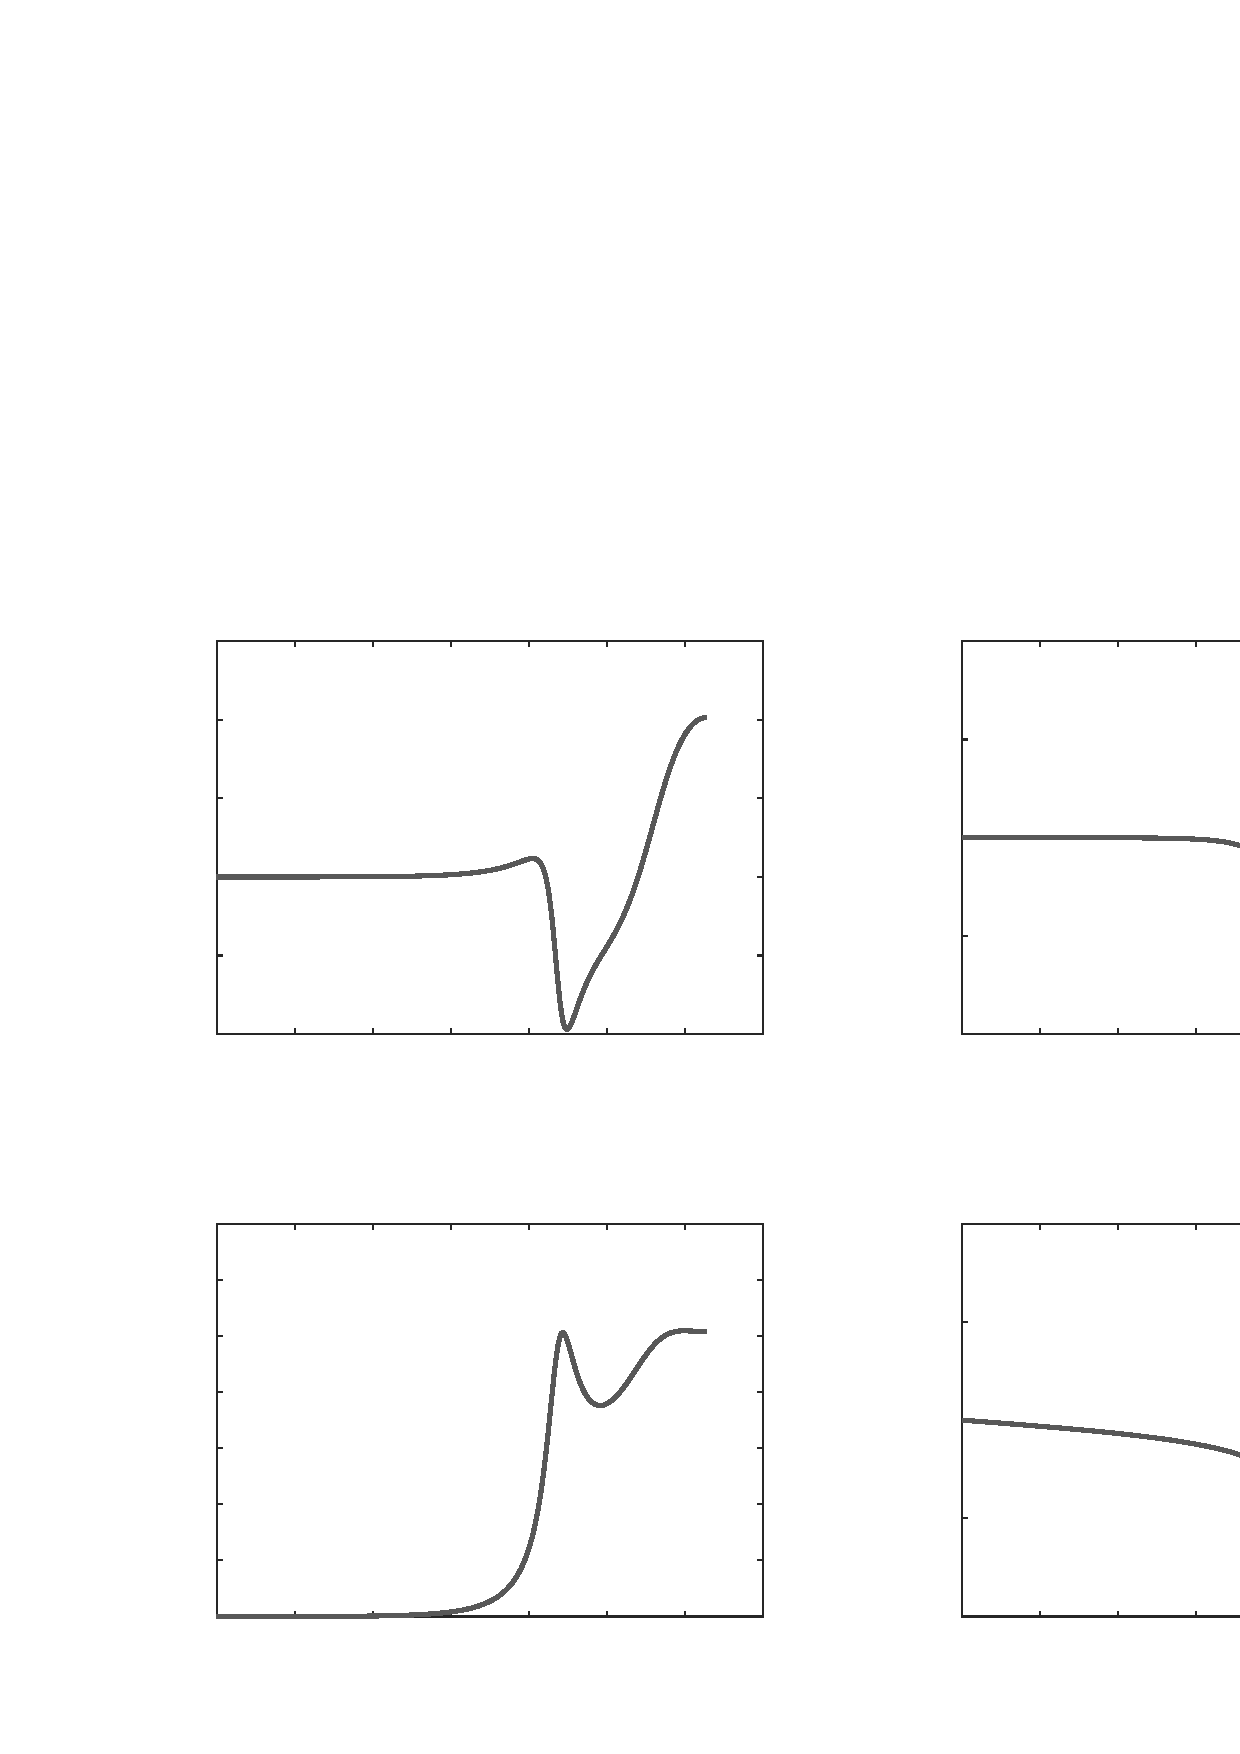
\includegraphics[scale=1]{octaves/dtft-example-inc}
\end{picture}%
\begin{picture}(800,600)(0,0)
\fontsize{13}{0}\selectfont\put(104,335.128){\makebox(0,0)[t]{\textcolor[rgb]{0.15,0.15,0.15}{{0}}}}
\fontsize{13}{0}\selectfont\put(141.438,335.128){\makebox(0,0)[t]{\textcolor[rgb]{0.15,0.15,0.15}{{0.5}}}}
\fontsize{13}{0}\selectfont\put(178.875,335.128){\makebox(0,0)[t]{\textcolor[rgb]{0.15,0.15,0.15}{{1}}}}
\fontsize{13}{0}\selectfont\put(216.313,335.128){\makebox(0,0)[t]{\textcolor[rgb]{0.15,0.15,0.15}{{1.5}}}}
\fontsize{13}{0}\selectfont\put(253.75,335.128){\makebox(0,0)[t]{\textcolor[rgb]{0.15,0.15,0.15}{{2}}}}
\fontsize{13}{0}\selectfont\put(291.188,335.128){\makebox(0,0)[t]{\textcolor[rgb]{0.15,0.15,0.15}{{2.5}}}}
\fontsize{13}{0}\selectfont\put(328.625,335.128){\makebox(0,0)[t]{\textcolor[rgb]{0.15,0.15,0.15}{{3}}}}
\fontsize{13}{0}\selectfont\put(366.063,335.128){\makebox(0,0)[t]{\textcolor[rgb]{0.15,0.15,0.15}{{3.5}}}}
\fontsize{13}{0}\selectfont\put(97.0508,345.577){\makebox(0,0)[r]{\textcolor[rgb]{0.15,0.15,0.15}{{-1}}}}
\fontsize{13}{0}\selectfont\put(97.0508,383.277){\makebox(0,0)[r]{\textcolor[rgb]{0.15,0.15,0.15}{{-0.5}}}}
\fontsize{13}{0}\selectfont\put(97.0508,420.977){\makebox(0,0)[r]{\textcolor[rgb]{0.15,0.15,0.15}{{0}}}}
\fontsize{13}{0}\selectfont\put(97.0508,458.677){\makebox(0,0)[r]{\textcolor[rgb]{0.15,0.15,0.15}{{0.5}}}}
\fontsize{13}{0}\selectfont\put(97.0508,496.377){\makebox(0,0)[r]{\textcolor[rgb]{0.15,0.15,0.15}{{1}}}}
\fontsize{13}{0}\selectfont\put(97.0508,534.077){\makebox(0,0)[r]{\textcolor[rgb]{0.15,0.15,0.15}{{1.5}}}}
\fontsize{15}{0}\selectfont\put(235.032,544.077){\makebox(0,0)[b]{\textcolor[rgb]{0,0,0}{{Real part of H}}}}
\fontsize{13}{0}\selectfont\put(461.937,335.128){\makebox(0,0)[t]{\textcolor[rgb]{0.15,0.15,0.15}{{0}}}}
\fontsize{13}{0}\selectfont\put(499.375,335.128){\makebox(0,0)[t]{\textcolor[rgb]{0.15,0.15,0.15}{{0.5}}}}
\fontsize{13}{0}\selectfont\put(536.812,335.128){\makebox(0,0)[t]{\textcolor[rgb]{0.15,0.15,0.15}{{1}}}}
\fontsize{13}{0}\selectfont\put(574.25,335.128){\makebox(0,0)[t]{\textcolor[rgb]{0.15,0.15,0.15}{{1.5}}}}
\fontsize{13}{0}\selectfont\put(611.687,335.128){\makebox(0,0)[t]{\textcolor[rgb]{0.15,0.15,0.15}{{2}}}}
\fontsize{13}{0}\selectfont\put(649.125,335.128){\makebox(0,0)[t]{\textcolor[rgb]{0.15,0.15,0.15}{{2.5}}}}
\fontsize{13}{0}\selectfont\put(686.562,335.128){\makebox(0,0)[t]{\textcolor[rgb]{0.15,0.15,0.15}{{3}}}}
\fontsize{13}{0}\selectfont\put(724,335.128){\makebox(0,0)[t]{\textcolor[rgb]{0.15,0.15,0.15}{{3.5}}}}
\fontsize{13}{0}\selectfont\put(454.988,345.577){\makebox(0,0)[r]{\textcolor[rgb]{0.15,0.15,0.15}{{-1}}}}
\fontsize{13}{0}\selectfont\put(454.988,392.702){\makebox(0,0)[r]{\textcolor[rgb]{0.15,0.15,0.15}{{-0.5}}}}
\fontsize{13}{0}\selectfont\put(454.988,439.827){\makebox(0,0)[r]{\textcolor[rgb]{0.15,0.15,0.15}{{0}}}}
\fontsize{13}{0}\selectfont\put(454.988,486.952){\makebox(0,0)[r]{\textcolor[rgb]{0.15,0.15,0.15}{{0.5}}}}
\fontsize{13}{0}\selectfont\put(454.988,534.077){\makebox(0,0)[r]{\textcolor[rgb]{0.15,0.15,0.15}{{1}}}}
\fontsize{15}{0}\selectfont\put(592.969,544.077){\makebox(0,0)[b]{\textcolor[rgb]{0,0,0}{{Imaginary part of H}}}}
\fontsize{13}{0}\selectfont\put(104,55.551){\makebox(0,0)[t]{\textcolor[rgb]{0.15,0.15,0.15}{{0}}}}
\fontsize{13}{0}\selectfont\put(141.438,55.551){\makebox(0,0)[t]{\textcolor[rgb]{0.15,0.15,0.15}{{0.5}}}}
\fontsize{13}{0}\selectfont\put(178.875,55.551){\makebox(0,0)[t]{\textcolor[rgb]{0.15,0.15,0.15}{{1}}}}
\fontsize{13}{0}\selectfont\put(216.313,55.551){\makebox(0,0)[t]{\textcolor[rgb]{0.15,0.15,0.15}{{1.5}}}}
\fontsize{13}{0}\selectfont\put(253.75,55.551){\makebox(0,0)[t]{\textcolor[rgb]{0.15,0.15,0.15}{{2}}}}
\fontsize{13}{0}\selectfont\put(291.188,55.551){\makebox(0,0)[t]{\textcolor[rgb]{0.15,0.15,0.15}{{2.5}}}}
\fontsize{13}{0}\selectfont\put(328.625,55.551){\makebox(0,0)[t]{\textcolor[rgb]{0.15,0.15,0.15}{{3}}}}
\fontsize{13}{0}\selectfont\put(366.063,55.551){\makebox(0,0)[t]{\textcolor[rgb]{0.15,0.15,0.15}{{3.5}}}}
\fontsize{13}{0}\selectfont\put(97.0508,66){\makebox(0,0)[r]{\textcolor[rgb]{0.15,0.15,0.15}{{0}}}}
\fontsize{13}{0}\selectfont\put(97.0508,92.9285){\makebox(0,0)[r]{\textcolor[rgb]{0.15,0.15,0.15}{{0.2}}}}
\fontsize{13}{0}\selectfont\put(97.0508,119.857){\makebox(0,0)[r]{\textcolor[rgb]{0.15,0.15,0.15}{{0.4}}}}
\fontsize{13}{0}\selectfont\put(97.0508,146.786){\makebox(0,0)[r]{\textcolor[rgb]{0.15,0.15,0.15}{{0.6}}}}
\fontsize{13}{0}\selectfont\put(97.0508,173.714){\makebox(0,0)[r]{\textcolor[rgb]{0.15,0.15,0.15}{{0.8}}}}
\fontsize{13}{0}\selectfont\put(97.0508,200.643){\makebox(0,0)[r]{\textcolor[rgb]{0.15,0.15,0.15}{{1}}}}
\fontsize{13}{0}\selectfont\put(97.0508,227.571){\makebox(0,0)[r]{\textcolor[rgb]{0.15,0.15,0.15}{{1.2}}}}
\fontsize{13}{0}\selectfont\put(97.0508,254.5){\makebox(0,0)[r]{\textcolor[rgb]{0.15,0.15,0.15}{{1.4}}}}
\fontsize{15}{0}\selectfont\put(235.032,264.5){\makebox(0,0)[b]{\textcolor[rgb]{0,0,0}{{Magnitude spectrum of H}}}}
\fontsize{13}{0}\selectfont\put(461.937,55.6063){\makebox(0,0)[t]{\textcolor[rgb]{0.15,0.15,0.15}{{0}}}}
\fontsize{13}{0}\selectfont\put(499.375,55.6063){\makebox(0,0)[t]{\textcolor[rgb]{0.15,0.15,0.15}{{0.5}}}}
\fontsize{13}{0}\selectfont\put(536.812,55.6063){\makebox(0,0)[t]{\textcolor[rgb]{0.15,0.15,0.15}{{1}}}}
\fontsize{13}{0}\selectfont\put(574.25,55.6063){\makebox(0,0)[t]{\textcolor[rgb]{0.15,0.15,0.15}{{1.5}}}}
\fontsize{13}{0}\selectfont\put(611.687,55.6063){\makebox(0,0)[t]{\textcolor[rgb]{0.15,0.15,0.15}{{2}}}}
\fontsize{13}{0}\selectfont\put(649.125,55.6063){\makebox(0,0)[t]{\textcolor[rgb]{0.15,0.15,0.15}{{2.5}}}}
\fontsize{13}{0}\selectfont\put(686.562,55.6063){\makebox(0,0)[t]{\textcolor[rgb]{0.15,0.15,0.15}{{3}}}}
\fontsize{13}{0}\selectfont\put(724,55.6063){\makebox(0,0)[t]{\textcolor[rgb]{0.15,0.15,0.15}{{3.5}}}}
\fontsize{13}{0}\selectfont\put(454.988,66){\makebox(0,0)[r]{\textcolor[rgb]{0.15,0.15,0.15}{{-4}}}}
\fontsize{13}{0}\selectfont\put(454.988,113.125){\makebox(0,0)[r]{\textcolor[rgb]{0.15,0.15,0.15}{{-2}}}}
\fontsize{13}{0}\selectfont\put(454.988,160.25){\makebox(0,0)[r]{\textcolor[rgb]{0.15,0.15,0.15}{{0}}}}
\fontsize{13}{0}\selectfont\put(454.988,207.375){\makebox(0,0)[r]{\textcolor[rgb]{0.15,0.15,0.15}{{2}}}}
\fontsize{13}{0}\selectfont\put(454.988,254.5){\makebox(0,0)[r]{\textcolor[rgb]{0.15,0.15,0.15}{{4}}}}
\fontsize{15}{0}\selectfont\put(592.969,264.5){\makebox(0,0)[b]{\textcolor[rgb]{0,0,0}{{Phase spectrum of H}}}}
\end{picture}

}\caption{\emph{Real part}, \emph{imaginary part}, \emph{magnitude spectrum} and \emph{phase spectrum} plots of Example~\ref{eqn:octaveExampleFreqz}. Notice the discontinuity in the $\arctan{}$ function that manifests with a sudden jump in the phase spectrum. Plots have been generated with the help of \texttt{octave}.}\label{oct:octaveExampleFreqz}
    \end{center}
\end{figure}
\clearpage

\subsection{The Unwrapped Phase Function}
In numerical computation when the computed phase function is outside of the possible range of $\omega$---that is $[-\pi, \pi]$---to bring the computed value to the correct range the phase is computed \emph{modulo} $2\pi$. Hence, the phase may exhibit some discontinuities of $2\pi$ radians in the phase spectrum plot, as in Figure~\ref{oct:octaveExampleFreqz}. Indeed, one would like to possess some kind of representation which doesn't present any kind of visible discontinuity; to do so, one should adopt the \textbf{unwrapped phase function}.

Unwrapped phase functions are special functions whose goal is to represent the phase without any dis\-con\-ti\-nui\-ty---that is, by \emph{unwrapping the phase}. Related function goes under the name of $\theta_c(\omega)$. In the following Figure~\ref{oct:octaveExampleFreqzUnwrap} the unwrapped phase spectrum has been plotted with the commands
\begin{verbatim}
plot(w,unwrap(angle(H)));
\end{verbatim}
which are enough to produce a plot of the desired unwrapped phase function of \texttt{H}.

% print -depslatex -mono "-S800,600" "figure-name.tex"
\begin{figure}[ht]
    \begin{center}
\scalebox{0.6}{
% Title: gl2ps_renderer figure
% Creator: GL2PS 1.4.2, (C) 1999-2020 C. Geuzaine
% For: Octave
% CreationDate: Wed Oct 19 08:41:45 2022
\setlength{\unitlength}{1pt}
\begin{picture}(0,0)
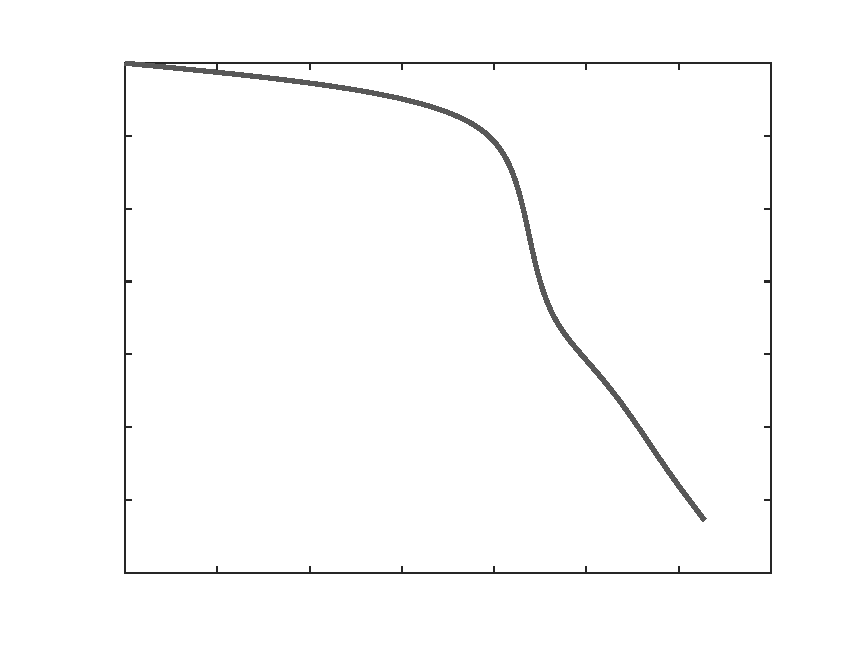
\includegraphics[scale=1]{octaves/dtft-unwrap-inc}
\end{picture}%
\begin{picture}(400,300)(0,0)
\fontsize{6}{0}\selectfont\put(52,27.7787){\makebox(0,0)[t]{\textcolor[rgb]{0.15,0.15,0.15}{{0}}}}
\fontsize{6}{0}\selectfont\put(96.2857,27.7787){\makebox(0,0)[t]{\textcolor[rgb]{0.15,0.15,0.15}{{0.5}}}}
\fontsize{6}{0}\selectfont\put(140.571,27.7787){\makebox(0,0)[t]{\textcolor[rgb]{0.15,0.15,0.15}{{1}}}}
\fontsize{6}{0}\selectfont\put(184.857,27.7787){\makebox(0,0)[t]{\textcolor[rgb]{0.15,0.15,0.15}{{1.5}}}}
\fontsize{6}{0}\selectfont\put(229.143,27.7787){\makebox(0,0)[t]{\textcolor[rgb]{0.15,0.15,0.15}{{2}}}}
\fontsize{6}{0}\selectfont\put(273.429,27.7787){\makebox(0,0)[t]{\textcolor[rgb]{0.15,0.15,0.15}{{2.5}}}}
\fontsize{6}{0}\selectfont\put(317.714,27.7787){\makebox(0,0)[t]{\textcolor[rgb]{0.15,0.15,0.15}{{3}}}}
\fontsize{6}{0}\selectfont\put(362,27.7787){\makebox(0,0)[t]{\textcolor[rgb]{0.15,0.15,0.15}{{3.5}}}}
\fontsize{6}{0}\selectfont\put(48.5263,33){\makebox(0,0)[r]{\textcolor[rgb]{0.15,0.15,0.15}{{-7}}}}
\fontsize{6}{0}\selectfont\put(48.5263,67.9286){\makebox(0,0)[r]{\textcolor[rgb]{0.15,0.15,0.15}{{-6}}}}
\fontsize{6}{0}\selectfont\put(48.5263,102.857){\makebox(0,0)[r]{\textcolor[rgb]{0.15,0.15,0.15}{{-5}}}}
\fontsize{6}{0}\selectfont\put(48.5263,137.786){\makebox(0,0)[r]{\textcolor[rgb]{0.15,0.15,0.15}{{-4}}}}
\fontsize{6}{0}\selectfont\put(48.5263,172.714){\makebox(0,0)[r]{\textcolor[rgb]{0.15,0.15,0.15}{{-3}}}}
\fontsize{6}{0}\selectfont\put(48.5263,207.643){\makebox(0,0)[r]{\textcolor[rgb]{0.15,0.15,0.15}{{-2}}}}
\fontsize{6}{0}\selectfont\put(48.5263,242.571){\makebox(0,0)[r]{\textcolor[rgb]{0.15,0.15,0.15}{{-1}}}}
\fontsize{6}{0}\selectfont\put(48.5263,277.5){\makebox(0,0)[r]{\textcolor[rgb]{0.15,0.15,0.15}{{0}}}}
\end{picture}

}\caption{\emph{Unwrapped} phase spectrum plot of phase spectrum of Example~\ref{eqn:octaveExampleFreqz}. By employing \texttt{unwrap} function in \texttt{octave}, the discontinuity in the $\arctan{}$ function had disappeared.}\label{oct:octaveExampleFreqzUnwrap}
    \end{center}
\end{figure}
Undeniably, the unwrapped representation remains imperative when plotting phase spectra.

\subsection{The Convolution Theorem}

The discrete-time Fourier transform (DTFT) is a form of Fourier analysis that is applicable to a sequence of values.

The DTFT is often used to analyze samples of a continuous function. The term discrete-time refers to the fact that the transform operates on discrete data, often samples whose interval has units of time. From uniformly spaced samples it produces a function of frequency that is a periodic summation of the continuous Fourier transform of the original continuous function. Under certain theoretical conditions, described by the sampling theorem, the original continuous function can be recovered perfectly from the DTFT and thus from the original discrete samples. The DTFT itself is a continuous function of frequency, but discrete samples of it can be readily calculated via the discrete Fourier transform (DFT), which is by far the most common method of modern Fourier analysis.

Indeed, a paramount property that surely helps when it comes to performing convolutions on the time-domain is the following, remarkable property, that goes under the name of \textbf{Convolution Theorem}.
\begin{thm}[Convolution Theorem]
    Consider two signals $g(x)$ and $h(x)$ whose Fourier Transforms are $G(\omega)$ and $H(\omega)$, and let $\mathcal F\{\cdot\}$ denote the operator of Fourier Transformation. The convolution of $g$ and $h$ is defined by
    \begin{equation}\label{eqn:convolutionTheorem}
        g \circledast h = \mathcal F^{-1}\{G \cdot H\},
    \end{equation}
    where a convolution sum in the time-domain corresponds to a \emph{product} in the frequency domain.
\end{thm}

The Convolution Theorem states that any convolution sum can be performed as a product in the frequency domain. This also means that no matter the signals' domain, jumping into the related frequency domain and performing a product of the Fourier Transforms of the two signals is a straightforward way to perform a convolution sum.
An immediate application of this crucial result is that the linear convolution $y[n]$ of $x[n]$ and $h[n]$ in a linear discrete-time system can be performed \emph{much} more quickly by going for the frequency-domain route. The steps of this faster process are the following ones,
\begin{enumerate}
    \item first, one computes the discrete-time Fourier Transforms of $x$ and $h$, that are $X(e^{j\omega})$ and $H(e^{j\omega})$;
    \item second, from the frequency-domain one quickly evaluates $Y(e^{j\omega}) = X(e^{j\omega})\cdot H(e^{j\omega})$;
    \item and at last, to obtain $y[n]$ it is enough to compute the inverse DTFT. The overall process is depicted in Figure~\ref{tikz:linearConvolutionFrequencyDomain}.
\end{enumerate}
\begin{figure}[ht]
\begin{center}
    \begin{tikzpicture}
    \node [](Xi){$x[n]$};
    \node [](Hi) at (0, -2){$h[n]$};
    \node [draw, boxfilter](DTFTX) at (2, 0) {DTFT};
    \node [draw, boxfilter](DTFTH) at (2, -2) {DTFT};
    \node [label=north:{$X(e^{j\omega})$}](X) at (3.3, 0){};
    \node [label=north:{$H(e^{j\omega})$}](H) at (3.3, -2){};
    \node [draw, circle, cross, thick, minimum size=.5cm](PROD) at (4, -1) {};
    \node [draw, boxfilter](IDTFTY) at (6, -1) {DTFT};
    \node [](Yo) at (7.5, -1){$y[n]$};

    \draw[-stealth] (Xi) -- (DTFTX);
    \draw[-stealth] (Hi) -- (DTFTH);
    \draw[-stealth] (DTFTX) -| (PROD);
    \draw[-stealth] (DTFTH) -| (PROD);
    \draw[-stealth] (PROD) -- (IDTFTY);
    \draw[-stealth] (IDTFTY) -- (Yo);
\end{tikzpicture}\caption{Linear convolution as a product in frequency domain. In reality, the process is not performed, as it is far from convenient to handle continuous signals.}\label{tikz:linearConvolutionFrequencyDomain}
\end{center}
\end{figure}

The aforementioned procedure is not feasible in reality for two reasons: first of all, it is never convenient---let alone possible---to effectively handle \emph{continuous} signals. Indeed, no machine can possibly compute all the infinite points required for the computation. Secondarily and not less importantly, the inverse discrete-time Fourier Transform is an \emph{integral}. Performing integrations on a continuous is far from efficient for the same reasons as above.

With the Convolution Theorem ends the chapter on Discrete-time Fourier Transforms. Indeed, as we will see, the Convolution Theorem will prove useful even for the next subject of study, the \emph{Discrete Fourier Transforms}.

\chapter{Discrete Fourier Transform}

In mathematics, the discrete Fourier transform (DFT) converts a finite sequence of equally-spaced samples of a function into a same-length sequence of equally-spaced samples of the discrete-time Fourier transform (DTFT), which is a complex-valued function of frequency. The interval at which the DTFT is sampled is the reciprocal of the duration of the input sequence. An inverse DFT is a Fourier series, using the DTFT samples as coefficients of complex sinusoids at the corresponding DTFT frequencies. It has the same sample-values as the original input sequence. The DFT is therefore said to be a frequency domain representation of the original input sequence. If the original sequence spans all the non-zero values of a function, its DTFT is continuous (and periodic), and the DFT provides discrete samples of one cycle. If the original sequence is one cycle of a periodic function, the DFT provides all the non-zero values of one DTFT cycle.

The DFT is the most important discrete transform, used to perform Fourier analysis in many practical applications. In digital signal processing, the function is any quantity or signal that varies over time, such as the pressure of a sound wave, a radio signal, or daily temperature readings, sampled over a finite time interval (often defined by a window function). In image processing, the samples can be the values of pixels along a row or column of a raster image. The DFT is also used to efficiently solve partial differential equations, and to perform other operations such as convolutions or multiplying large integers.

Since it deals with a \textbf{finite} amount of data, it can be implemented in computers by numerical algorithms or even dedicated hardware. These implementations usually employ efficient fast Fourier transform (FFT) algorithms; so much so that the terms ``FFT'' and ``DFT'' are often used interchangeably. Prior to its current usage, the ``FFT'' initialism may have also been used for the ambiguous term ``finite Fourier transform''~\cite{bib:discreteFourierTransform}.

\section{Orthogonal Transforms}

Let $x[n]$ be a sequence of length $N$. We define $\mathcal X[k], 0 \leq k \leq N-1$ the $N$-point \textbf{orthogonal transform} of $x[n]$. An orthogonal transforms is a \emph{generalized} version of Transforms that takes the form
\begin{eqnarray}
    \mathcal X[k] = \sum_{n=0}^{N-1} x[n] \psi^*[k,n], & 0 \leq k \leq N-1, \\\label{eqn:analysisEquation}
    x[k] = \sum_{k=0}^{N-1} \mathcal X[n] \psi[k,n], & 0 \leq n \leq N-1. \label{eqn:synthesisEquation}
\end{eqnarray}
The first Equation~\ref{eqn:analysisEquation} is called \emph{Analysis equation}, while the second Equation~\ref{eqn:synthesisEquation} is said to be the \emph{Synthesis equation}. Both analysis and synthesis equations concur in the definition of the orthogonal transform. Indeed, the analysis equation allows to perform the orthogonal transformation, while implicitly the synthesis equation serves as a ``inverse'' orthogonal transform. Still, the $\psi$ are said to be \emph{basis sequences} and are of length $N$ as well as the original sequence and the orthogonal transform sequence. Basis sequences can have complex values, so generally $\psi[k, n] \in \C$. In the class of transforms to be considered in this notes of digital signal processing, all the basis sequences will satisfy the following condition,
\begin{equation}\label{eqn:orthogonalTransformsOrthogonalityCondition}
    \frac 1 N \sum_{n=0}^{N-1} \psi[k,n]\psi^*[l,n] = \left\{\begin{array}{ll}1, & l = k\\ 0, & l \neq k\end{array}\right.,
\end{equation}
a condition that substantially poses that the product \[\psi[k,n]\psi^*[l,n]\] is equal to $1$ if and only if indexes $l = k$, a property that if satisfied then the basis sequences are said to be \emph{orthogonal to each other}.

Really, in order for $\psi^*$ to be the inverse orthogonal transform, $\psi$ and $\psi^*$ have to be orthogonal to each other. This can be verified by substituting the synthesis equation~\ref{eqn:synthesisEquation} into the analysis equation~\ref{eqn:analysisEquation},
\begin{align*}
    \sum_{n=0}^{N-1} x[n] \psi^*[k,n] &= \sum_{n=0}^{N-1}\left( \frac 1 N \sum_{k=0}^{N-1} \mathcal X[k] \psi[n,k]\right)\psi^*[l,n] \\
                                      &= \sum_{k=0}^{N-1} \mathcal X[k] \left( \frac 1 N \sum_{n=0}^{N-1}\psi[n,k]\psi^*[l,n]\right) \\
                                      &= \mathcal X[l],
\end{align*}
which yields an identity. Of course, the other way around works exactly the same, hence the inverse orthogonal transform is expressed as in Equation~\ref{eqn:synthesisEquation}.

An important consequence of the orthogonality condition for orthogonal transforms is the \textbf{Energy Preservation Property}, which states that
\begin{equation}\label{eqn:energyPreservationProperty}
    \sum_{n=0}^{N-1}|x[n]|^2 = \frac 1 N \sum_{k=0}^{N-1}\left|\mathcal X[n]\right|^2
\end{equation}
Yet, the Energy Preservation Property is more commonly known as the \emph{Parseval's Theorem}, of which it is a more general formulation.

\section{Definition of Discrete Fourier Transform}

It's now the time to introduce the \textbf{Discrete Fourier Transform (DFT)}, a tool of a paramount importance in the field of digital signal processing.

\begin{defin}[Discrete Fourier Transform]
    Let $x[n]$ be a finite-length sequence of length $N$ defined for $0 \leq n \leq N-1$ and be $X(e^{j\omega})$ its discrete-time Fourier Transform as in Equation~\ref{eqn:discreteTimeFourierTransform}. By \emph{uniformly sampling} $X(e^{j\omega})$ on the $\omega$ axis in the interval $[0, 2\pi[$ at samples $\omega_k=\frac{2k\pi}{N}$ for $0 \leq k \leq N-1$ one obtains a sequence $X[k]$ such that
    \begin{equation}\label{eqn:discreteFourierTransform}
        X[k] = X(e^{j\omega})\Bigr\rvert_{\omega = \frac {2k\pi}{N}} = \sum_{n=0}^{N-1} x[n] e^{-2j\pi \frac{k n}{N}}, 0 \leq k \leq N-1
    \end{equation}
    where $X[k]$ is a sequence of length $N$ in the frequency domain represented by the variable $k$. The sequence $X[k]$ is called the \emph{Discrete Fourier Transform (DFT)} of the sequence.
\end{defin}

The above definition has been obtained by sampling the $\omega$ frequency variable in samples $2k\pi / N$ so that the complex continuous exponential $e^{-j\omega}$ has become $e^{-2j\pi \frac{kn}{N}}$. Usually, in order to streamline the notation, the substitution
\begin{equation}\label{eqn:dftNotationWn}
    W_N = e^{-j\frac{2\pi}{N}}
\end{equation}
under which the Discrete Fourier Transform now is rewritten into the following,
\begin{equation}\label{eqn:discreteTimeFourierTransformWn}
        X[k] = \sum_{n=0}^{N-1} x[n] W_N^{kn}, 0 \leq k \leq N-1.
\end{equation}

The notation expressed in~\ref{eqn:dftNotationWn} renders the orthogonal transform operator $W_N$ in Discrete Fourier Transform sum have a positive sign in its exponents. This behavior is the opposite of what one encounters by looking at the original definition.

Along with the DFT, the \textbf{Inverse Discrete Fourier Transform} should be defined as well in order to produce meaningful computations. Indeed,
\begin{equation}\label{eqn:inverseDiscreteFourierTransformWn}
    x[k] = \sum_{k=0}^{N-1} X[k] W_N^{-kn}, 0 \leq n \leq N-1,
\end{equation}
expressed under the new notation\footnote{
    The original Discrete Fourier Transform---without employing the new notation---would be 
    \[
        x[k] = \sum_{k=0}^{N-1} X[k] e^{2j\pi\frac{kn}{N}}, 0 \leq n \leq N-1,
    \]
    showing a positive sign at the exponentiation.
}.
Verifying the above inverse transform is straightforward, as it is enough to substitute the original transform into the inverse, then multiply both sides of the equation by $W_N^{ln}$ and sum the result from $n=0$ to $n=N-1$. Of course,
\begin{align*}
    \sum_{n=0}^{N-1} x[n] W_N^{ln}
    &= \sum_{n=0}^{N-1}\left(\frac 1 N\sum_{k=0}^{K-1} X[k] W_N^{-kn}\right)W_n^{ln}\\
    &= \frac 1 N \sum_{n=0}^{N-1}\sum_{k=0}^{K-1} X[k] W_N^{-(k-l)n}\\
    &= \frac 1 N \sum_{k=0}^{K-1} X[k] \left(\sum_{n=0}^{N-1}W_N^{-(k-l)n}\right).
\end{align*}
Now, since
\begin{equation}\label{eqn:dftWnProperty}
    \sum_{n=0}^{N-1}W_N^{-(k-l)n} = \left\{\begin{array}{ll} N, & k - l = rN, r \in \Z\\ 0, & \mbox{otherwise}\end{array}\right.
\end{equation}
due to the exponentiation properties. In order to verify that, just substitute with the definition of $W_N$, that is \[\sum_{n=0}^{N-1}e^{+2j\pi\frac{(k-l)n}{N}},\] a quantity that indeed is equal to $N$ if and only if $k-l$ is a multiple of $N$ and $0$ otherwise. The term relative to $n=0$ is the sum of $N$ terms all equal to $1$, while the term for $n\neq 0$ is related to the first $N$ terms of a geometric progression, that are \[\sum_{n=0}^{N-1}\rho^n = \frac{1-\rho^N}{1 - \rho} = 0\] as the exponential $e^{j2\pi\frac{N}{N}} = 1$. Another way to see it is to consider that a set of $W_N$ vectors is summed together---when $k\neq l$ for each vector of phase $\varphi$ another vector of opposite phase $-\varphi$ is summed, and the result of the sum is exactly $0$; on contrary, the only way to avoid the cancellation of terms is when $k = l$, that is when all terms have magnitude equal to $|e^{j2\pi\frac{N}{N}}| = 1$ and possess phase $\varphi = 0$. For this reason, one obtains that the only non-zero term in the sum is $\sum_{n=0}^{N-1} W_N^{-(k-l)n}, k=l, 0\leq l,k \leq N-1$. Hence,
\begin{align*}
    \sum_{n=0}^{N-1} x[n] W_N^{ln}
    &= \frac 1 N \sum_{k=0}^{K-1} X[k] \left(\sum_{n=0}^{N-1}W_N^{-(k-l)n}\right).\\
    &= \frac 1 N X[l] N = X[l].
\end{align*}

The first example in exam is a DFT of the following sequence of length $N$,
\[
    x[n] = \left\{\begin{array}{ll} 
            1 & n=0\\
            0 & 1 \leq n \leq N-1
        \end{array}\right.
\]
that is quite similar to the delta impulse. Its $N$-point Discrete Fourier Transform is given by
\[
    X[k] = \sum_{n=0}^{N-1} x[n]W_N^{kn} = x[0]W_N^{k0} = 1, 1\leq k \leq N-1.
\]

The second example is of a sequence
\[
    y[n] = \left\{\begin{array}{ll} 
            1 & n=m\\
            0 & 0\leq n \leq m-1, m+1 \leq n \leq N-1
        \end{array}\right.
\]
which is like the previous example, but translated of $m$. Its Discrete Fourier Transform will be
\[
    Y[k] = \sum_{n=0}^{N-1} y[n]W_N^{kn} = y[m]W_N^{km} = W_N^{km}, 1\leq k \leq N-1.
\]

Let now $g[n] = \cos{2\pi \frac{rn}{N}}$ be a sequence of length $N$. Since
\begin{align*}
    g[n] &= \frac 1 2 \left(e^{j2\pi \frac{rn}{N}} + e^{-j2\pi \frac{rn}{N}}\right)\\
         &= \frac 1 2 \left(W_N^{rn} + W_N^{rn}\right),
\end{align*}
and due to linearity the Discrete Fourier Transform will be the transform of the two addends. Therefore,
\begin{align*}
    G[k] &= \sum_{n=0}^{N-1} g[n] W_N^{kn} \\
         &= \frac 1 2 \left(\sum_{n=0}^{N-1} W_N^{-(r-k)n} + \sum_{n=0}^{N-1} W_N^{-(r+k)n}\right)
\end{align*}
and by means of Identity~\ref{eqn:dftWnProperty} one finally obtains that
\[
    G[k] = \left\{\begin{array}{ll}
            \frac N 2 & k = r\\
            \frac N 2 & k = N - r\\
            0         & \mbox{ otherwise }
    \end{array}\right.
\]

The DFT of a cosine wave is a pair of impulses of amplitude $\frac N 2$, located at samples $r$ and $N-r$ that represent \emph{the same} frequency. Conceptually then, a cosine DFT is a pair of impulses just like in the case of the Discrete-time Fourier Transform.

\subsection{Matrix relations}

Discrete Fourier Transform as expressed in~\ref{eqn:discreteTimeFourierTransformWn} can be easily expressed into a matrix form. Let $\bm x$ and $\bm X$ be two column vectors as defined,
\[
    \bm{x} = \begin{bmatrix} x[0] \\ x[1] \\ \vdots \\ x[N-1] \end{bmatrix}
    \bm{X} = \begin{bmatrix} X[0] \\ X[1] \\ \vdots \\ X[N-1] \end{bmatrix}
\]
the \emph{Matrix form of the Discrete Fourier Transform} is
\begin{equation}\label{eqn:dftMatrixForm}
    \bm{X} = \bm{D}_N\bm{x}
\end{equation}
with $\bm D_N$ the \textbf{DFT Matrix}, a $N \times N$ matrix given by
\begin{equation}\label{eqn:dftMatrixDn}
    \bm D_N = \begin{bmatrix}
        1 & 1 & 1 & \cdots & 1 \\
        1 & W_N^1 & W_N^2 & \cdots & W_N^{(N-1)} \\
        1 & W_N^2 & W_N^4 & \cdots & W_N^{2(N-1)} \\
        \vdots & \vdots & \vdots & \ddots & \vdots \\
        1 & W_N^{(N-1)} & W_N^{2(N-1)} & \cdots & W_N^{(N-1)^2} \\
    \end{bmatrix}
\end{equation}

Conversely, the \emph{Matrix form of the Inverse Discrete Fourier Transform} is given by a similar relationship,
\begin{equation}\label{eqn:idftMatrixForm}
    \bm{x} = \bm{D}^{-1}_N\bm{X}
\end{equation}
with $\bm D_N$ the \textbf{Inverse DFT Matrix}, a $N \times N$ matrix given by
\begin{equation}\label{eqn:idftMatrixDn}
    \bm D^{-1}_N = \frac 1 N\begin{bmatrix}
        1 & 1 & 1 & \cdots & 1 \\
        1 & W_N^{-1} & W_N^{-2} & \cdots & W_N^{-(N-1)} \\
        1 & W_N^{-2} & W_N^{-4} & \cdots & W_N^{-2(N-1)} \\
        \vdots & \vdots & \vdots & \ddots & \vdots \\
        1 & W_N^{-(N-1)} & W_N^{-2(N-1)} & \cdots & W_N^{-(N-1)^2} \\
    \end{bmatrix}
\end{equation}

Remarkably, the following relationship holds between the inverse and the straight DFT Matrix,
\[
    \bm D_N = \frac 1 N \bm D^{-1}_N,
\]
with a factor of $\frac 1 N$ between the one and the other.

Matrix relations are crucial to learn how to manipulate Discrete Fourier Transforms in \textsc{Matlab}. In fact, the two functions \texttt{fft} and \texttt{ifft}---which stand for \emph{Fast Fourier Transform} and \emph{Inverse Fast Fourier Transform}---manipulate column vector data structures. These two functions make use of sophisticated techniques and efficient algorithms based on the ``dividi et impera'' concept to optimize the computation of the DFT.

Let's study the DFT of the cosine $\cos{2\pi r \frac{n}{N}}$. The following \texttt{octave} code computes and plots the DFT of such function, first by setting $r=3$, then with $r=3.3$.
\begin{verbatim}
N = 21;
M = 21;
r = 3; n = 0:N-1;  u = cos(2*pi*r*n/N);
U = fft(u,M);
figure(1);
subplot(2,3,1);   n = 0:1:N-1;   stem(n,u);
title('Original time-domain sequence'); 
xlabel('Time index n'); ylabel('Amplitude')
subplot(2,3,2);   k = 0:1:M-1;   stem(k,abs(U));
title('Magnitude, r = 3'); 
xlabel('Frequency index k'); ylabel('Magnitude')
subplot(2,3,3);   stem(k,angle(U));
title('Phase, r = 3'); 
xlabel('Frequency index k'); ylabel('Phase')
\end{verbatim}

\begin{verbatim}
r = 3.3; n = 0:N-1;  u = cos(2*pi*r*n/N); 
U = fft(u,M);
subplot(2,3,4);   n = 0:1:N-1;   stem(n,u);
title('Original time-domain sequence'); 
xlabel('Time index n'); ylabel('Amplitude')
subplot(2,3,5);   k = 0:1:M-1;   stem(k,abs(U));
title('Magnitude, r = 3.3'); 
xlabel('Frequency index k'); ylabel('Magnitude')
subplot(2,3,6);   stem(k,angle(U));
title('Phase, r = 3.3'); 
xlabel('Frequency index k'); ylabel('Phase')
\end{verbatim}

\begin{figure*}[ht]
\begin{center}
\scalebox{0.6}{
% Title: gl2ps_renderer figure
% Creator: GL2PS 1.4.2, (C) 1999-2020 C. Geuzaine
% For: Octave
% CreationDate: Wed Oct 19 16:31:04 2022
\setlength{\unitlength}{1pt}
\begin{picture}(0,0)
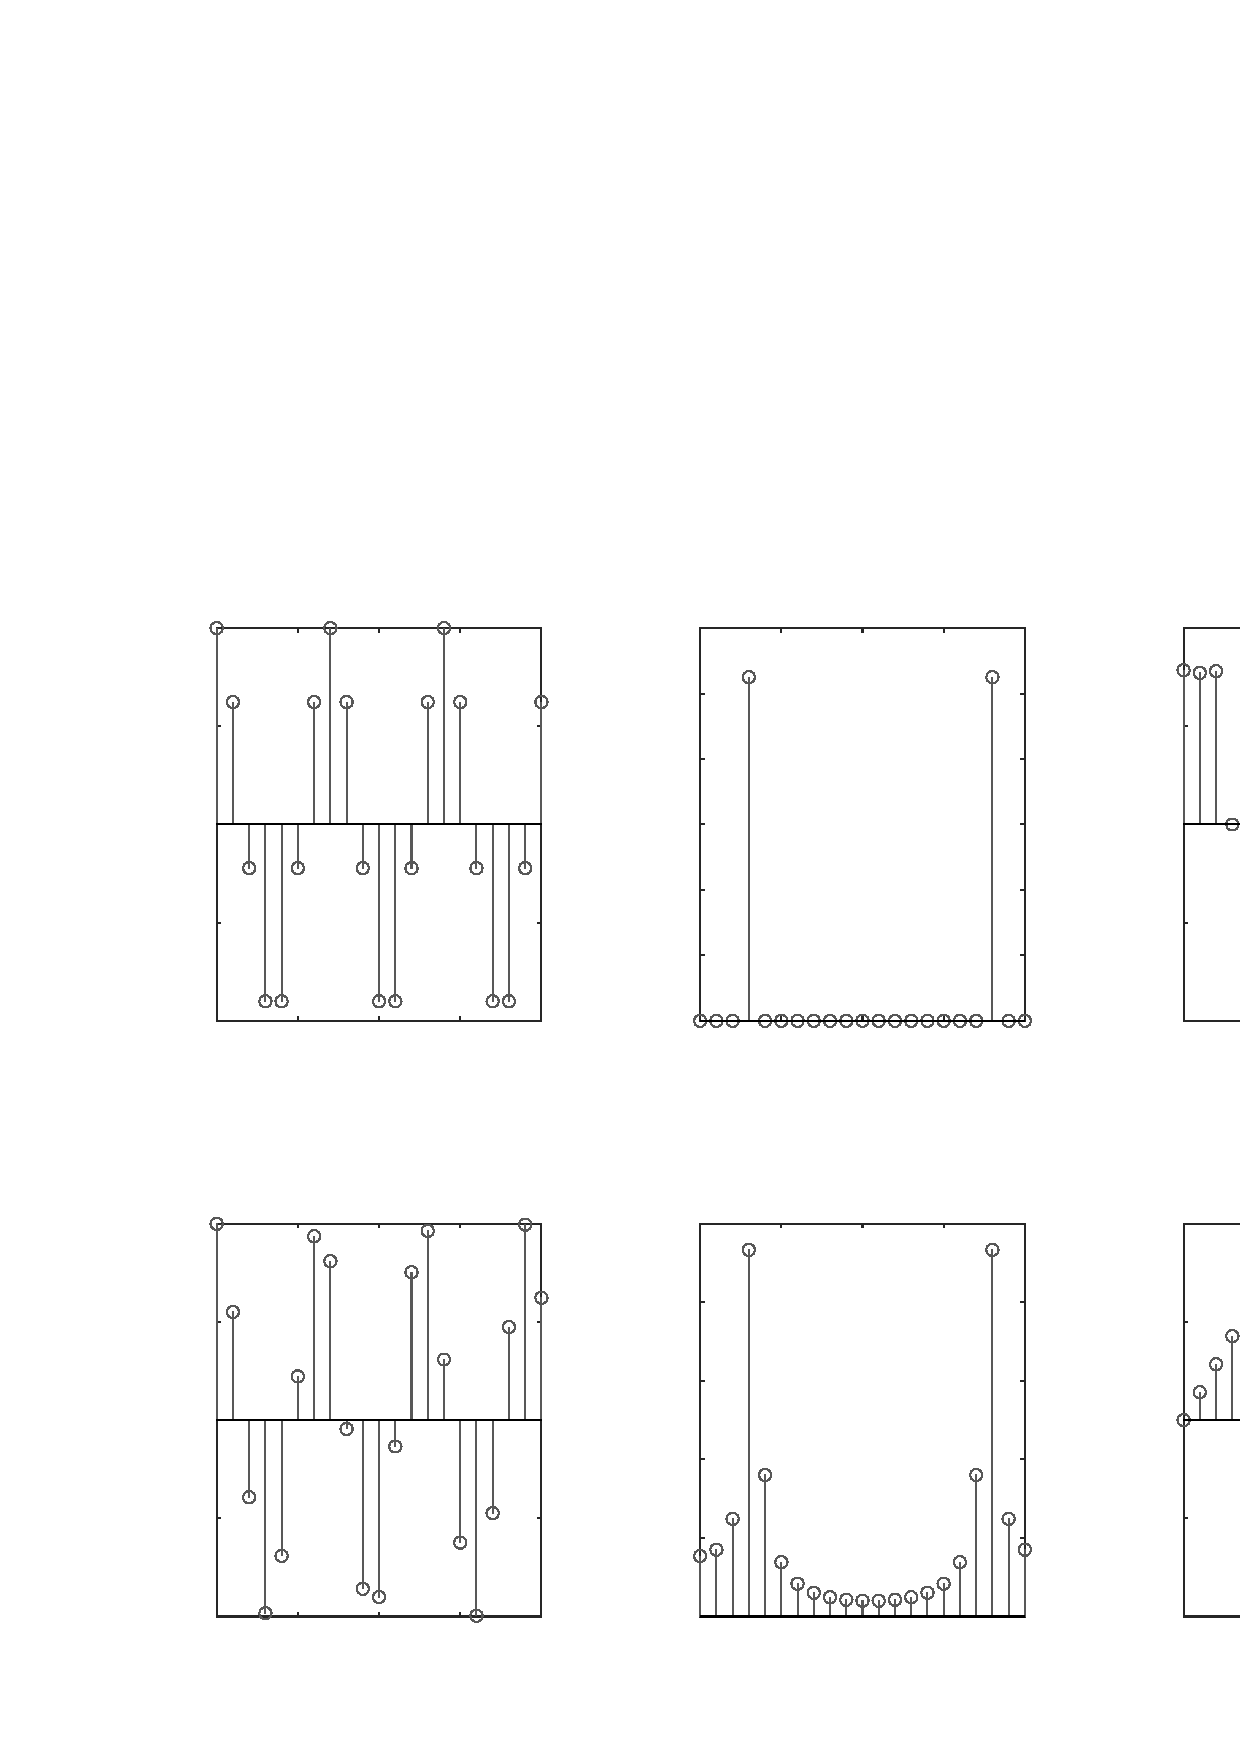
\includegraphics[scale=1]{octaves/dftCosine-inc}
\end{picture}%
\begin{picture}(800,600)(0,0)
\fontsize{13}{0}\selectfont\put(104,341.53){\makebox(0,0)[t]{\textcolor[rgb]{0.15,0.15,0.15}{{0}}}}
\fontsize{13}{0}\selectfont\put(142.97,341.53){\makebox(0,0)[t]{\textcolor[rgb]{0.15,0.15,0.15}{{5}}}}
\fontsize{13}{0}\selectfont\put(181.94,341.53){\makebox(0,0)[t]{\textcolor[rgb]{0.15,0.15,0.15}{{10}}}}
\fontsize{13}{0}\selectfont\put(220.91,341.53){\makebox(0,0)[t]{\textcolor[rgb]{0.15,0.15,0.15}{{15}}}}
\fontsize{13}{0}\selectfont\put(259.88,341.53){\makebox(0,0)[t]{\textcolor[rgb]{0.15,0.15,0.15}{{20}}}}
\fontsize{13}{0}\selectfont\put(97.0579,351.924){\makebox(0,0)[r]{\textcolor[rgb]{0.15,0.15,0.15}{{-1}}}}
\fontsize{13}{0}\selectfont\put(97.0579,399.049){\makebox(0,0)[r]{\textcolor[rgb]{0.15,0.15,0.15}{{-0.5}}}}
\fontsize{13}{0}\selectfont\put(97.0579,446.174){\makebox(0,0)[r]{\textcolor[rgb]{0.15,0.15,0.15}{{0}}}}
\fontsize{13}{0}\selectfont\put(97.0579,493.299){\makebox(0,0)[r]{\textcolor[rgb]{0.15,0.15,0.15}{{0.5}}}}
\fontsize{13}{0}\selectfont\put(97.0579,540.424){\makebox(0,0)[r]{\textcolor[rgb]{0.15,0.15,0.15}{{1}}}}
\fontsize{15}{0}\selectfont\put(181.94,550.424){\makebox(0,0)[b]{\textcolor[rgb]{0,0,0}{{Original time-domain sequence}}}}
\fontsize{15}{0}\selectfont\put(68.0579,446.174){\rotatebox{90}{\makebox(0,0)[b]{\textcolor[rgb]{0.15,0.15,0.15}{{Amplitude}}}}}
\fontsize{15}{0}\selectfont\put(181.94,325.53){\makebox(0,0)[t]{\textcolor[rgb]{0.15,0.15,0.15}{{Time index n}}}}
\fontsize{13}{0}\selectfont\put(336.06,341.53){\makebox(0,0)[t]{\textcolor[rgb]{0.15,0.15,0.15}{{0}}}}
\fontsize{13}{0}\selectfont\put(375.03,341.53){\makebox(0,0)[t]{\textcolor[rgb]{0.15,0.15,0.15}{{5}}}}
\fontsize{13}{0}\selectfont\put(414,341.53){\makebox(0,0)[t]{\textcolor[rgb]{0.15,0.15,0.15}{{10}}}}
\fontsize{13}{0}\selectfont\put(452.97,341.53){\makebox(0,0)[t]{\textcolor[rgb]{0.15,0.15,0.15}{{15}}}}
\fontsize{13}{0}\selectfont\put(491.94,341.53){\makebox(0,0)[t]{\textcolor[rgb]{0.15,0.15,0.15}{{20}}}}
\fontsize{13}{0}\selectfont\put(329.118,351.924){\makebox(0,0)[r]{\textcolor[rgb]{0.15,0.15,0.15}{{0}}}}
\fontsize{13}{0}\selectfont\put(329.118,383.34){\makebox(0,0)[r]{\textcolor[rgb]{0.15,0.15,0.15}{{2}}}}
\fontsize{13}{0}\selectfont\put(329.118,414.757){\makebox(0,0)[r]{\textcolor[rgb]{0.15,0.15,0.15}{{4}}}}
\fontsize{13}{0}\selectfont\put(329.118,446.174){\makebox(0,0)[r]{\textcolor[rgb]{0.15,0.15,0.15}{{6}}}}
\fontsize{13}{0}\selectfont\put(329.118,477.59){\makebox(0,0)[r]{\textcolor[rgb]{0.15,0.15,0.15}{{8}}}}
\fontsize{13}{0}\selectfont\put(329.118,509.007){\makebox(0,0)[r]{\textcolor[rgb]{0.15,0.15,0.15}{{10}}}}
\fontsize{13}{0}\selectfont\put(329.118,540.424){\makebox(0,0)[r]{\textcolor[rgb]{0.15,0.15,0.15}{{12}}}}
\fontsize{15}{0}\selectfont\put(414,550.424){\makebox(0,0)[b]{\textcolor[rgb]{0,0,0}{{Magnitude, r = 3}}}}
\fontsize{15}{0}\selectfont\put(308.118,446.174){\rotatebox{90}{\makebox(0,0)[b]{\textcolor[rgb]{0.15,0.15,0.15}{{Magnitude}}}}}
\fontsize{15}{0}\selectfont\put(414,325.53){\makebox(0,0)[t]{\textcolor[rgb]{0.15,0.15,0.15}{{Frequency index k}}}}
\fontsize{13}{0}\selectfont\put(568.12,341.53){\makebox(0,0)[t]{\textcolor[rgb]{0.15,0.15,0.15}{{0}}}}
\fontsize{13}{0}\selectfont\put(607.09,341.53){\makebox(0,0)[t]{\textcolor[rgb]{0.15,0.15,0.15}{{5}}}}
\fontsize{13}{0}\selectfont\put(646.06,341.53){\makebox(0,0)[t]{\textcolor[rgb]{0.15,0.15,0.15}{{10}}}}
\fontsize{13}{0}\selectfont\put(685.03,341.53){\makebox(0,0)[t]{\textcolor[rgb]{0.15,0.15,0.15}{{15}}}}
\fontsize{13}{0}\selectfont\put(724,341.53){\makebox(0,0)[t]{\textcolor[rgb]{0.15,0.15,0.15}{{20}}}}
\fontsize{13}{0}\selectfont\put(561.178,351.924){\makebox(0,0)[r]{\textcolor[rgb]{0.15,0.15,0.15}{{-4}}}}
\fontsize{13}{0}\selectfont\put(561.178,399.049){\makebox(0,0)[r]{\textcolor[rgb]{0.15,0.15,0.15}{{-2}}}}
\fontsize{13}{0}\selectfont\put(561.178,446.174){\makebox(0,0)[r]{\textcolor[rgb]{0.15,0.15,0.15}{{0}}}}
\fontsize{13}{0}\selectfont\put(561.178,493.299){\makebox(0,0)[r]{\textcolor[rgb]{0.15,0.15,0.15}{{2}}}}
\fontsize{13}{0}\selectfont\put(561.178,540.424){\makebox(0,0)[r]{\textcolor[rgb]{0.15,0.15,0.15}{{4}}}}
\fontsize{15}{0}\selectfont\put(646.06,550.424){\makebox(0,0)[b]{\textcolor[rgb]{0,0,0}{{Phase, r = 3}}}}
\fontsize{15}{0}\selectfont\put(543.178,446.174){\rotatebox{90}{\makebox(0,0)[b]{\textcolor[rgb]{0.15,0.15,0.15}{{Phase}}}}}
\fontsize{15}{0}\selectfont\put(646.06,325.53){\makebox(0,0)[t]{\textcolor[rgb]{0.15,0.15,0.15}{{Frequency index k}}}}
\fontsize{13}{0}\selectfont\put(104,55.6063){\makebox(0,0)[t]{\textcolor[rgb]{0.15,0.15,0.15}{{0}}}}
\fontsize{13}{0}\selectfont\put(142.97,55.6063){\makebox(0,0)[t]{\textcolor[rgb]{0.15,0.15,0.15}{{5}}}}
\fontsize{13}{0}\selectfont\put(181.94,55.6063){\makebox(0,0)[t]{\textcolor[rgb]{0.15,0.15,0.15}{{10}}}}
\fontsize{13}{0}\selectfont\put(220.91,55.6063){\makebox(0,0)[t]{\textcolor[rgb]{0.15,0.15,0.15}{{15}}}}
\fontsize{13}{0}\selectfont\put(259.88,55.6063){\makebox(0,0)[t]{\textcolor[rgb]{0.15,0.15,0.15}{{20}}}}
\fontsize{13}{0}\selectfont\put(97.0579,66){\makebox(0,0)[r]{\textcolor[rgb]{0.15,0.15,0.15}{{-1}}}}
\fontsize{13}{0}\selectfont\put(97.0579,113.125){\makebox(0,0)[r]{\textcolor[rgb]{0.15,0.15,0.15}{{-0.5}}}}
\fontsize{13}{0}\selectfont\put(97.0579,160.25){\makebox(0,0)[r]{\textcolor[rgb]{0.15,0.15,0.15}{{0}}}}
\fontsize{13}{0}\selectfont\put(97.0579,207.375){\makebox(0,0)[r]{\textcolor[rgb]{0.15,0.15,0.15}{{0.5}}}}
\fontsize{13}{0}\selectfont\put(97.0579,254.5){\makebox(0,0)[r]{\textcolor[rgb]{0.15,0.15,0.15}{{1}}}}
\fontsize{15}{0}\selectfont\put(181.94,264.5){\makebox(0,0)[b]{\textcolor[rgb]{0,0,0}{{Original time-domain sequence}}}}
\fontsize{15}{0}\selectfont\put(68.0579,160.25){\rotatebox{90}{\makebox(0,0)[b]{\textcolor[rgb]{0.15,0.15,0.15}{{Amplitude}}}}}
\fontsize{15}{0}\selectfont\put(181.94,39.6063){\makebox(0,0)[t]{\textcolor[rgb]{0.15,0.15,0.15}{{Time index n}}}}
\fontsize{13}{0}\selectfont\put(336.06,55.6063){\makebox(0,0)[t]{\textcolor[rgb]{0.15,0.15,0.15}{{0}}}}
\fontsize{13}{0}\selectfont\put(375.03,55.6063){\makebox(0,0)[t]{\textcolor[rgb]{0.15,0.15,0.15}{{5}}}}
\fontsize{13}{0}\selectfont\put(414,55.6063){\makebox(0,0)[t]{\textcolor[rgb]{0.15,0.15,0.15}{{10}}}}
\fontsize{13}{0}\selectfont\put(452.97,55.6063){\makebox(0,0)[t]{\textcolor[rgb]{0.15,0.15,0.15}{{15}}}}
\fontsize{13}{0}\selectfont\put(491.94,55.6063){\makebox(0,0)[t]{\textcolor[rgb]{0.15,0.15,0.15}{{20}}}}
\fontsize{13}{0}\selectfont\put(329.118,66){\makebox(0,0)[r]{\textcolor[rgb]{0.15,0.15,0.15}{{0}}}}
\fontsize{13}{0}\selectfont\put(329.118,103.7){\makebox(0,0)[r]{\textcolor[rgb]{0.15,0.15,0.15}{{2}}}}
\fontsize{13}{0}\selectfont\put(329.118,141.4){\makebox(0,0)[r]{\textcolor[rgb]{0.15,0.15,0.15}{{4}}}}
\fontsize{13}{0}\selectfont\put(329.118,179.1){\makebox(0,0)[r]{\textcolor[rgb]{0.15,0.15,0.15}{{6}}}}
\fontsize{13}{0}\selectfont\put(329.118,216.8){\makebox(0,0)[r]{\textcolor[rgb]{0.15,0.15,0.15}{{8}}}}
\fontsize{13}{0}\selectfont\put(329.118,254.5){\makebox(0,0)[r]{\textcolor[rgb]{0.15,0.15,0.15}{{10}}}}
\fontsize{15}{0}\selectfont\put(414,264.5){\makebox(0,0)[b]{\textcolor[rgb]{0,0,0}{{Magnitude, r = 3.3}}}}
\fontsize{15}{0}\selectfont\put(308.118,160.25){\rotatebox{90}{\makebox(0,0)[b]{\textcolor[rgb]{0.15,0.15,0.15}{{Magnitude}}}}}
\fontsize{15}{0}\selectfont\put(414,39.6063){\makebox(0,0)[t]{\textcolor[rgb]{0.15,0.15,0.15}{{Frequency index k}}}}
\fontsize{13}{0}\selectfont\put(568.12,55.6063){\makebox(0,0)[t]{\textcolor[rgb]{0.15,0.15,0.15}{{0}}}}
\fontsize{13}{0}\selectfont\put(607.09,55.6063){\makebox(0,0)[t]{\textcolor[rgb]{0.15,0.15,0.15}{{5}}}}
\fontsize{13}{0}\selectfont\put(646.06,55.6063){\makebox(0,0)[t]{\textcolor[rgb]{0.15,0.15,0.15}{{10}}}}
\fontsize{13}{0}\selectfont\put(685.03,55.6063){\makebox(0,0)[t]{\textcolor[rgb]{0.15,0.15,0.15}{{15}}}}
\fontsize{13}{0}\selectfont\put(724,55.6063){\makebox(0,0)[t]{\textcolor[rgb]{0.15,0.15,0.15}{{20}}}}
\fontsize{13}{0}\selectfont\put(561.178,66){\makebox(0,0)[r]{\textcolor[rgb]{0.15,0.15,0.15}{{-2}}}}
\fontsize{13}{0}\selectfont\put(561.178,113.125){\makebox(0,0)[r]{\textcolor[rgb]{0.15,0.15,0.15}{{-1}}}}
\fontsize{13}{0}\selectfont\put(561.178,160.25){\makebox(0,0)[r]{\textcolor[rgb]{0.15,0.15,0.15}{{0}}}}
\fontsize{13}{0}\selectfont\put(561.178,207.375){\makebox(0,0)[r]{\textcolor[rgb]{0.15,0.15,0.15}{{1}}}}
\fontsize{13}{0}\selectfont\put(561.178,254.5){\makebox(0,0)[r]{\textcolor[rgb]{0.15,0.15,0.15}{{2}}}}
\fontsize{15}{0}\selectfont\put(646.06,264.5){\makebox(0,0)[b]{\textcolor[rgb]{0,0,0}{{Phase, r = 3.3}}}}
\fontsize{15}{0}\selectfont\put(543.178,160.25){\rotatebox{90}{\makebox(0,0)[b]{\textcolor[rgb]{0.15,0.15,0.15}{{Phase}}}}}
\fontsize{15}{0}\selectfont\put(646.06,39.6063){\makebox(0,0)[t]{\textcolor[rgb]{0.15,0.15,0.15}{{Frequency index k}}}}
\end{picture}

}\caption{Plots of original signal (left), magnitude (center) and phase (right) of the Discrete Fourier Transform of sequence $\cos{2\pi r \frac{n}{N}}$. Notice how two perfect impulses are generated if and only if the quantity $r$ is an integer.}\label{oct:dftCosine}
\end{center}
\end{figure*}

The Discrete Fourier Transform of a cosine wave will produce a peculiar \emph{pair of impulses} located at the very same frequency of the sinusoid, provided the multiplying factor of $n$ is a \emph{multiple of $2\pi$}---that is, when $r \in \Z$. In all other cases, imperfect impulses will be generated, a phenomenon that is quite visible in Figure~\ref{oct:dftCosine} for the case of $r=3.3$.

The DFT of the delta impulse can be produced by running the following \texttt{octave} code, that will first generate three pictures like those in Figure~\ref{oct:dftCosine} related to a $\delta[n]$ sequence, then it will do the same with a delayed delta impulse,
\begin{verbatim}
N = 21;
M = 21;
u = [1 zeros(1,N-1)];
U = fft(u,M);
figure(1);
subplot(2,3,1);   n = 0:1:N-1;   stem(n,u);
title('Impulse in zero'); 
xlabel('Time index n'); ylabel('Amplitude')
subplot(2,3,2);   k = 0:1:M-1;   stem(k,abs(U));
title('Magnitude'); 
xlabel('Frequency index k'); ylabel('Magnitude')
subplot(2,3,3);   stem(k,angle(U));
title('Phase'); 
xlabel('Frequency index k'); ylabel('Phase')
\end{verbatim}

\begin{verbatim}
u = [zeros(1,4) 1 zeros(1,N-5)]; 
U = fft(u,M);
subplot(2,3,4);   n = 0:1:N-1;   stem(n,u);
title('Delayed impulse'); 
xlabel('Time index n'); ylabel('Amplitude')
subplot(2,3,5);   k = 0:1:M-1;   stem(k,abs(U));
title('Magnitude'); 
xlabel('Frequency index k'); ylabel('Magnitude')
subplot(2,3,6);   stem(k,angle(U));
title('Phase'); 
xlabel('Frequency index k'); ylabel('Phase')
\end{verbatim}



\begin{figure*}[ht]
\begin{center}
\scalebox{0.6}{
% Title: gl2ps_renderer figure
% Creator: GL2PS 1.4.2, (C) 1999-2020 C. Geuzaine
% For: Octave
% CreationDate: Wed Oct 19 16:35:19 2022
\setlength{\unitlength}{1pt}
\begin{picture}(0,0)
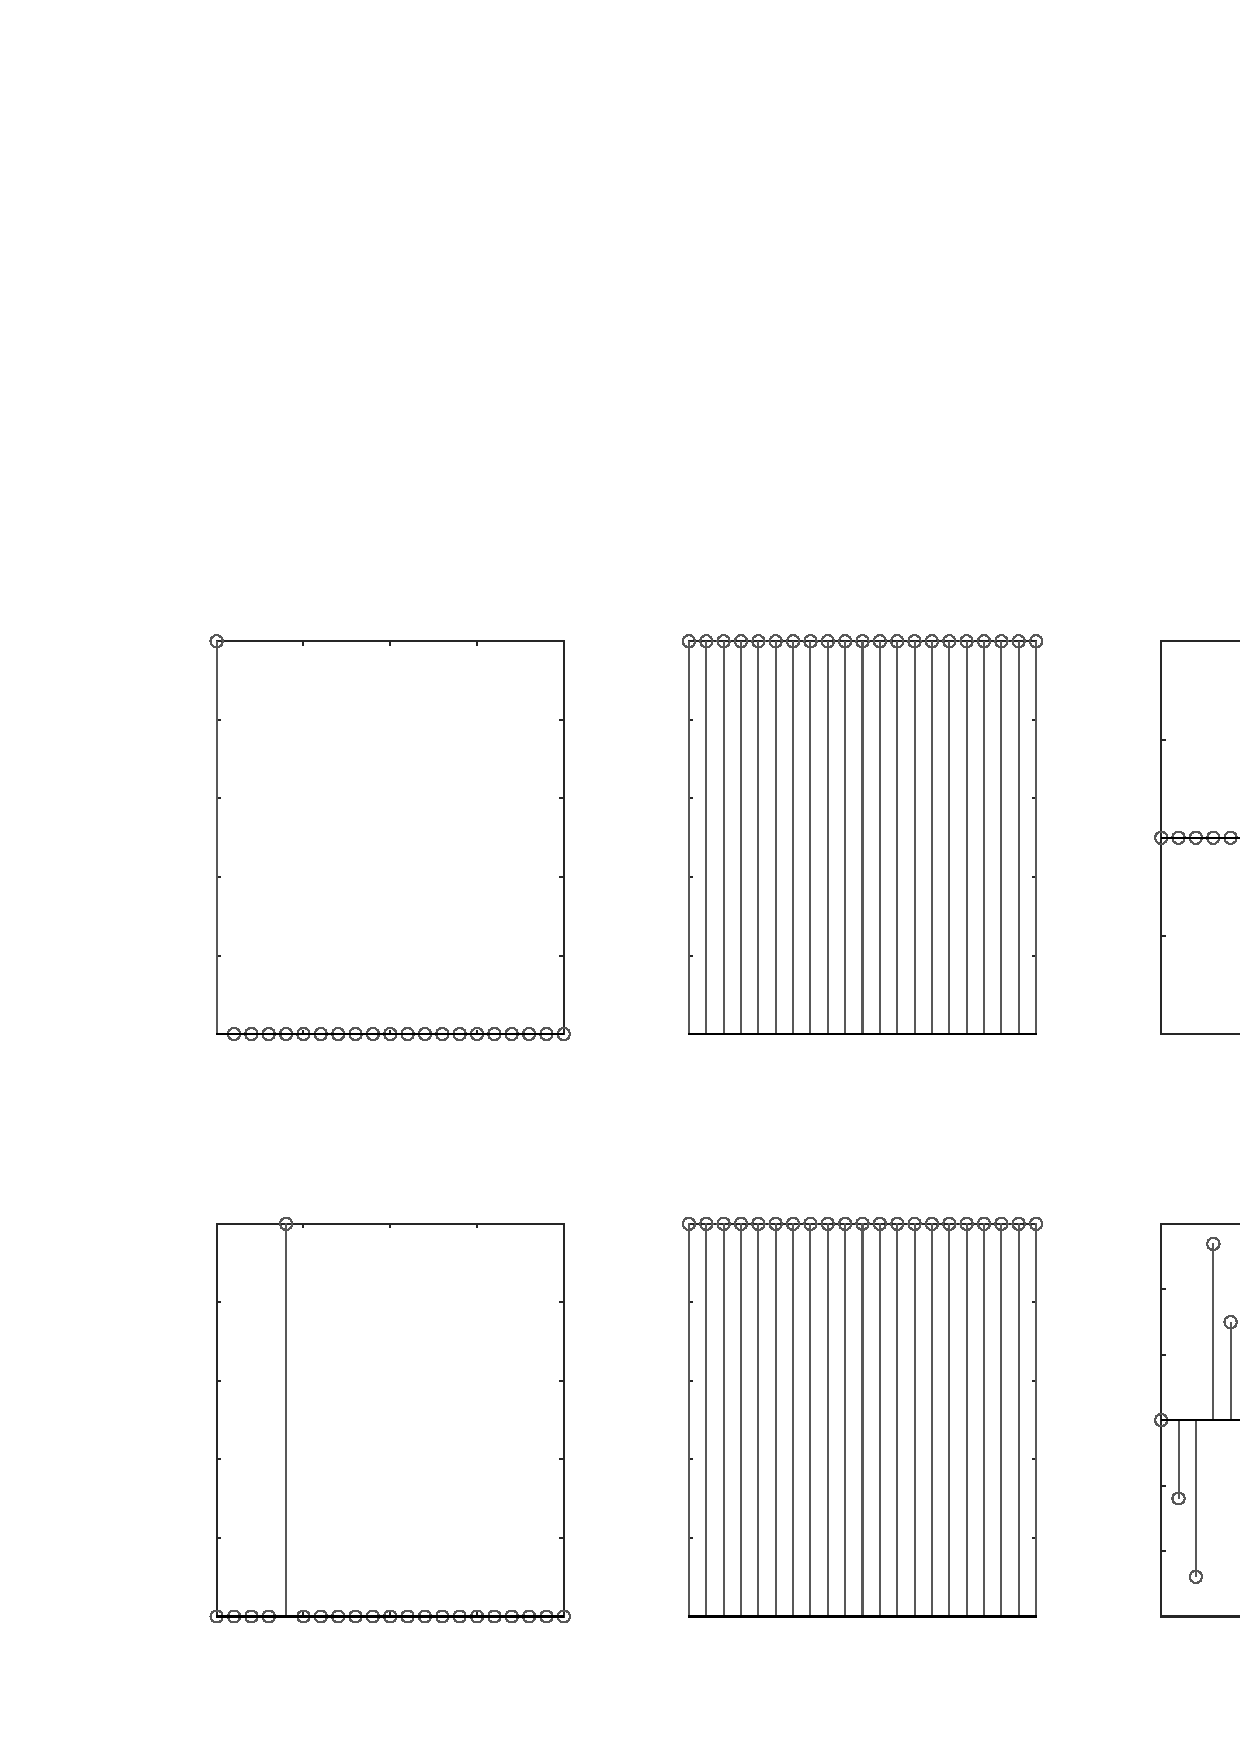
\includegraphics[scale=1]{octaves/dftImpulse-inc}
\end{picture}%
\begin{picture}(800,600)(0,0)
\fontsize{13}{0}\selectfont\put(104,335.173){\makebox(0,0)[t]{\textcolor[rgb]{0.15,0.15,0.15}{{0}}}}
\fontsize{13}{0}\selectfont\put(145.658,335.173){\makebox(0,0)[t]{\textcolor[rgb]{0.15,0.15,0.15}{{5}}}}
\fontsize{13}{0}\selectfont\put(187.316,335.173){\makebox(0,0)[t]{\textcolor[rgb]{0.15,0.15,0.15}{{10}}}}
\fontsize{13}{0}\selectfont\put(228.973,335.173){\makebox(0,0)[t]{\textcolor[rgb]{0.15,0.15,0.15}{{15}}}}
\fontsize{13}{0}\selectfont\put(270.631,335.173){\makebox(0,0)[t]{\textcolor[rgb]{0.15,0.15,0.15}{{20}}}}
\fontsize{13}{0}\selectfont\put(97.0679,345.566){\makebox(0,0)[r]{\textcolor[rgb]{0.15,0.15,0.15}{{0}}}}
\fontsize{13}{0}\selectfont\put(97.0679,383.266){\makebox(0,0)[r]{\textcolor[rgb]{0.15,0.15,0.15}{{0.2}}}}
\fontsize{13}{0}\selectfont\put(97.0679,420.966){\makebox(0,0)[r]{\textcolor[rgb]{0.15,0.15,0.15}{{0.4}}}}
\fontsize{13}{0}\selectfont\put(97.0679,458.666){\makebox(0,0)[r]{\textcolor[rgb]{0.15,0.15,0.15}{{0.6}}}}
\fontsize{13}{0}\selectfont\put(97.0679,496.366){\makebox(0,0)[r]{\textcolor[rgb]{0.15,0.15,0.15}{{0.8}}}}
\fontsize{13}{0}\selectfont\put(97.0679,534.066){\makebox(0,0)[r]{\textcolor[rgb]{0.15,0.15,0.15}{{1}}}}
\fontsize{15}{0}\selectfont\put(187.316,319.173){\makebox(0,0)[t]{\textcolor[rgb]{0.15,0.15,0.15}{{Time index n}}}}
\fontsize{15}{0}\selectfont\put(73.0679,439.816){\rotatebox{90}{\makebox(0,0)[b]{\textcolor[rgb]{0.15,0.15,0.15}{{Amplitude}}}}}
\fontsize{15}{0}\selectfont\put(187.316,544.066){\makebox(0,0)[b]{\textcolor[rgb]{0,0,0}{{Impulse in zero}}}}
\fontsize{13}{0}\selectfont\put(330.684,335.173){\makebox(0,0)[t]{\textcolor[rgb]{0.15,0.15,0.15}{{0}}}}
\fontsize{13}{0}\selectfont\put(372.342,335.173){\makebox(0,0)[t]{\textcolor[rgb]{0.15,0.15,0.15}{{5}}}}
\fontsize{13}{0}\selectfont\put(414,335.173){\makebox(0,0)[t]{\textcolor[rgb]{0.15,0.15,0.15}{{10}}}}
\fontsize{13}{0}\selectfont\put(455.658,335.173){\makebox(0,0)[t]{\textcolor[rgb]{0.15,0.15,0.15}{{15}}}}
\fontsize{13}{0}\selectfont\put(497.316,335.173){\makebox(0,0)[t]{\textcolor[rgb]{0.15,0.15,0.15}{{20}}}}
\fontsize{13}{0}\selectfont\put(323.752,345.566){\makebox(0,0)[r]{\textcolor[rgb]{0.15,0.15,0.15}{{0}}}}
\fontsize{13}{0}\selectfont\put(323.752,383.266){\makebox(0,0)[r]{\textcolor[rgb]{0.15,0.15,0.15}{{0.2}}}}
\fontsize{13}{0}\selectfont\put(323.752,420.966){\makebox(0,0)[r]{\textcolor[rgb]{0.15,0.15,0.15}{{0.4}}}}
\fontsize{13}{0}\selectfont\put(323.752,458.666){\makebox(0,0)[r]{\textcolor[rgb]{0.15,0.15,0.15}{{0.6}}}}
\fontsize{13}{0}\selectfont\put(323.752,496.366){\makebox(0,0)[r]{\textcolor[rgb]{0.15,0.15,0.15}{{0.8}}}}
\fontsize{13}{0}\selectfont\put(323.752,534.066){\makebox(0,0)[r]{\textcolor[rgb]{0.15,0.15,0.15}{{1}}}}
\fontsize{15}{0}\selectfont\put(414,319.173){\makebox(0,0)[t]{\textcolor[rgb]{0.15,0.15,0.15}{{Frequency index k}}}}
\fontsize{15}{0}\selectfont\put(299.752,439.816){\rotatebox{90}{\makebox(0,0)[b]{\textcolor[rgb]{0.15,0.15,0.15}{{Magnitude}}}}}
\fontsize{15}{0}\selectfont\put(414,544.066){\makebox(0,0)[b]{\textcolor[rgb]{0,0,0}{{Magnitude}}}}
\fontsize{13}{0}\selectfont\put(557.369,335.173){\makebox(0,0)[t]{\textcolor[rgb]{0.15,0.15,0.15}{{0}}}}
\fontsize{13}{0}\selectfont\put(599.027,335.173){\makebox(0,0)[t]{\textcolor[rgb]{0.15,0.15,0.15}{{5}}}}
\fontsize{13}{0}\selectfont\put(640.684,335.173){\makebox(0,0)[t]{\textcolor[rgb]{0.15,0.15,0.15}{{10}}}}
\fontsize{13}{0}\selectfont\put(682.342,335.173){\makebox(0,0)[t]{\textcolor[rgb]{0.15,0.15,0.15}{{15}}}}
\fontsize{13}{0}\selectfont\put(724,335.173){\makebox(0,0)[t]{\textcolor[rgb]{0.15,0.15,0.15}{{20}}}}
\fontsize{13}{0}\selectfont\put(550.437,345.566){\makebox(0,0)[r]{\textcolor[rgb]{0.15,0.15,0.15}{{-1}}}}
\fontsize{13}{0}\selectfont\put(550.437,392.691){\makebox(0,0)[r]{\textcolor[rgb]{0.15,0.15,0.15}{{-0.5}}}}
\fontsize{13}{0}\selectfont\put(550.437,439.816){\makebox(0,0)[r]{\textcolor[rgb]{0.15,0.15,0.15}{{0}}}}
\fontsize{13}{0}\selectfont\put(550.437,486.941){\makebox(0,0)[r]{\textcolor[rgb]{0.15,0.15,0.15}{{0.5}}}}
\fontsize{13}{0}\selectfont\put(550.437,534.066){\makebox(0,0)[r]{\textcolor[rgb]{0.15,0.15,0.15}{{1}}}}
\fontsize{15}{0}\selectfont\put(640.684,319.173){\makebox(0,0)[t]{\textcolor[rgb]{0.15,0.15,0.15}{{Frequency index k}}}}
\fontsize{15}{0}\selectfont\put(521.437,439.816){\rotatebox{90}{\makebox(0,0)[b]{\textcolor[rgb]{0.15,0.15,0.15}{{Phase}}}}}
\fontsize{15}{0}\selectfont\put(640.684,544.066){\makebox(0,0)[b]{\textcolor[rgb]{0,0,0}{{Phase}}}}
\fontsize{13}{0}\selectfont\put(104,55.6063){\makebox(0,0)[t]{\textcolor[rgb]{0.15,0.15,0.15}{{0}}}}
\fontsize{13}{0}\selectfont\put(145.658,55.6063){\makebox(0,0)[t]{\textcolor[rgb]{0.15,0.15,0.15}{{5}}}}
\fontsize{13}{0}\selectfont\put(187.316,55.6063){\makebox(0,0)[t]{\textcolor[rgb]{0.15,0.15,0.15}{{10}}}}
\fontsize{13}{0}\selectfont\put(228.973,55.6063){\makebox(0,0)[t]{\textcolor[rgb]{0.15,0.15,0.15}{{15}}}}
\fontsize{13}{0}\selectfont\put(270.631,55.6063){\makebox(0,0)[t]{\textcolor[rgb]{0.15,0.15,0.15}{{20}}}}
\fontsize{13}{0}\selectfont\put(97.0679,66){\makebox(0,0)[r]{\textcolor[rgb]{0.15,0.15,0.15}{{0}}}}
\fontsize{13}{0}\selectfont\put(97.0679,103.7){\makebox(0,0)[r]{\textcolor[rgb]{0.15,0.15,0.15}{{0.2}}}}
\fontsize{13}{0}\selectfont\put(97.0679,141.4){\makebox(0,0)[r]{\textcolor[rgb]{0.15,0.15,0.15}{{0.4}}}}
\fontsize{13}{0}\selectfont\put(97.0679,179.1){\makebox(0,0)[r]{\textcolor[rgb]{0.15,0.15,0.15}{{0.6}}}}
\fontsize{13}{0}\selectfont\put(97.0679,216.8){\makebox(0,0)[r]{\textcolor[rgb]{0.15,0.15,0.15}{{0.8}}}}
\fontsize{13}{0}\selectfont\put(97.0679,254.5){\makebox(0,0)[r]{\textcolor[rgb]{0.15,0.15,0.15}{{1}}}}
\fontsize{15}{0}\selectfont\put(187.316,39.6063){\makebox(0,0)[t]{\textcolor[rgb]{0.15,0.15,0.15}{{Time index n}}}}
\fontsize{15}{0}\selectfont\put(73.0679,160.25){\rotatebox{90}{\makebox(0,0)[b]{\textcolor[rgb]{0.15,0.15,0.15}{{Amplitude}}}}}
\fontsize{15}{0}\selectfont\put(187.316,264.5){\makebox(0,0)[b]{\textcolor[rgb]{0,0,0}{{Delayed impulse}}}}
\fontsize{13}{0}\selectfont\put(330.684,55.6063){\makebox(0,0)[t]{\textcolor[rgb]{0.15,0.15,0.15}{{0}}}}
\fontsize{13}{0}\selectfont\put(372.342,55.6063){\makebox(0,0)[t]{\textcolor[rgb]{0.15,0.15,0.15}{{5}}}}
\fontsize{13}{0}\selectfont\put(414,55.6063){\makebox(0,0)[t]{\textcolor[rgb]{0.15,0.15,0.15}{{10}}}}
\fontsize{13}{0}\selectfont\put(455.658,55.6063){\makebox(0,0)[t]{\textcolor[rgb]{0.15,0.15,0.15}{{15}}}}
\fontsize{13}{0}\selectfont\put(497.316,55.6063){\makebox(0,0)[t]{\textcolor[rgb]{0.15,0.15,0.15}{{20}}}}
\fontsize{13}{0}\selectfont\put(323.752,66){\makebox(0,0)[r]{\textcolor[rgb]{0.15,0.15,0.15}{{0}}}}
\fontsize{13}{0}\selectfont\put(323.752,103.7){\makebox(0,0)[r]{\textcolor[rgb]{0.15,0.15,0.15}{{0.2}}}}
\fontsize{13}{0}\selectfont\put(323.752,141.4){\makebox(0,0)[r]{\textcolor[rgb]{0.15,0.15,0.15}{{0.4}}}}
\fontsize{13}{0}\selectfont\put(323.752,179.1){\makebox(0,0)[r]{\textcolor[rgb]{0.15,0.15,0.15}{{0.6}}}}
\fontsize{13}{0}\selectfont\put(323.752,216.8){\makebox(0,0)[r]{\textcolor[rgb]{0.15,0.15,0.15}{{0.8}}}}
\fontsize{13}{0}\selectfont\put(323.752,254.5){\makebox(0,0)[r]{\textcolor[rgb]{0.15,0.15,0.15}{{1}}}}
\fontsize{15}{0}\selectfont\put(414,39.6063){\makebox(0,0)[t]{\textcolor[rgb]{0.15,0.15,0.15}{{Frequency index k}}}}
\fontsize{15}{0}\selectfont\put(299.752,160.25){\rotatebox{90}{\makebox(0,0)[b]{\textcolor[rgb]{0.15,0.15,0.15}{{Magnitude}}}}}
\fontsize{15}{0}\selectfont\put(414,264.5){\makebox(0,0)[b]{\textcolor[rgb]{0,0,0}{{Magnitude}}}}
\fontsize{13}{0}\selectfont\put(557.369,55.6063){\makebox(0,0)[t]{\textcolor[rgb]{0.15,0.15,0.15}{{0}}}}
\fontsize{13}{0}\selectfont\put(599.027,55.6063){\makebox(0,0)[t]{\textcolor[rgb]{0.15,0.15,0.15}{{5}}}}
\fontsize{13}{0}\selectfont\put(640.684,55.6063){\makebox(0,0)[t]{\textcolor[rgb]{0.15,0.15,0.15}{{10}}}}
\fontsize{13}{0}\selectfont\put(682.342,55.6063){\makebox(0,0)[t]{\textcolor[rgb]{0.15,0.15,0.15}{{15}}}}
\fontsize{13}{0}\selectfont\put(724,55.6063){\makebox(0,0)[t]{\textcolor[rgb]{0.15,0.15,0.15}{{20}}}}
\fontsize{13}{0}\selectfont\put(550.437,66){\makebox(0,0)[r]{\textcolor[rgb]{0.15,0.15,0.15}{{-3}}}}
\fontsize{13}{0}\selectfont\put(550.437,97.4166){\makebox(0,0)[r]{\textcolor[rgb]{0.15,0.15,0.15}{{-2}}}}
\fontsize{13}{0}\selectfont\put(550.437,128.833){\makebox(0,0)[r]{\textcolor[rgb]{0.15,0.15,0.15}{{-1}}}}
\fontsize{13}{0}\selectfont\put(550.437,160.25){\makebox(0,0)[r]{\textcolor[rgb]{0.15,0.15,0.15}{{0}}}}
\fontsize{13}{0}\selectfont\put(550.437,191.667){\makebox(0,0)[r]{\textcolor[rgb]{0.15,0.15,0.15}{{1}}}}
\fontsize{13}{0}\selectfont\put(550.437,223.083){\makebox(0,0)[r]{\textcolor[rgb]{0.15,0.15,0.15}{{2}}}}
\fontsize{13}{0}\selectfont\put(550.437,254.5){\makebox(0,0)[r]{\textcolor[rgb]{0.15,0.15,0.15}{{3}}}}
\fontsize{15}{0}\selectfont\put(640.684,39.6063){\makebox(0,0)[t]{\textcolor[rgb]{0.15,0.15,0.15}{{Frequency index k}}}}
\fontsize{15}{0}\selectfont\put(532.437,160.25){\rotatebox{90}{\makebox(0,0)[b]{\textcolor[rgb]{0.15,0.15,0.15}{{Phase}}}}}
\fontsize{15}{0}\selectfont\put(640.684,264.5){\makebox(0,0)[b]{\textcolor[rgb]{0,0,0}{{Phase}}}}
\end{picture}

}\caption{Plots of original signal (left), magnitude (center) and phase (right) of the Discrete Fourier Transform of sequences $\delta[n]$ and $\delta[n-4]$. The magnitude of the DFT is a constant as the transform of a delta will be a constant.}\label{oct:dftImpulse}
\end{center}
\end{figure*}

\subsection{Sampling process of a Discrete Fourier Transform}

Consider a sequence $x[n]$ whose Discrete-time Fourier Transform is $X(e^{j\omega})$. In order to obtain the Discrete Fourier Transform, one has to sample the DTFT at equally spaced points $\omega_k = \frac{2k\pi}{N}$ with $0 \leq k \leq N-1$, developing the frequency samples $\{X(e^{j\omega_k})\}$---these frequency samples can be considered the $N$-point DFT $Y[k]$ whose $N$-point IDFT is a sequence $y[n]$ of length $N$. This is because sampling a Discrete-time Fourier Transform will result in a Discrete Fourier Transform \emph{provided} the sampling is applied in $N$ points. That way, \[\{X(e^{j\omega_k})\} = Y[k].\]
Now, since the Discrete-time Fourier Transform is, like in Equation~\ref{eqn:inverseDiscreteTimeFourierTransform}
\[
    X(e^{j\omega}) = \sum_{l=-\infty}^\infty x[l] e^{-j\omega l};
\]
this leads to
\begin{align*}
    Y[k]
    &=  X(e^{j\omega_k}) = X\left(e^{j2\pi \frac k N}\right)\\
    &= \sum_{l=-\infty}^\infty x[l] e^{-j2\pi \frac{kl}{N}}\\
    &= \sum_{l=-\infty}^\infty x[l]W_N^{kl}.
\end{align*}

The trick now is to compute the IDFT of $y[n]$ and substitute the just obtained expression for $Y[k]$. That is,
\begin{align*}
    y[n]
    &= \frac 1 N \sum_{k=0}^{N-1} Y[k] W_N^{-kn}\\
    &= \frac 1 N \sum_{k=0}^{N-1}\sum_{l=-\infty}^\infty x[l]W_N^{kl} W_N^{-kn}\\
    &= \sum_{l=-\infty}^\infty\left(\frac 1 N \sum_{k=0}^{N-1} x[l]W_N^{-k(n-l)}\right);
\end{align*}
by means of the following identity
\begin{equation}\label{eqn:dftWnPropertyTwo}
    \sum_{n=0}^{N-1}W_N^{-k(n-l)} = \left\{\begin{array}{ll} N, & l = n + mN, \\ 0, & \mbox{otherwise}\end{array}\right.
\end{equation}
which is analogous of~\ref{eqn:dftWnProperty}, one soon obtains the desired relation
\begin{equation}\label{eqn:dftInfiniteReplicas}
    y[n] = \sum_{m=-\infty}^{\infty} x[n + mN], 0 \leq n \leq N-1.
\end{equation}

This last result, expressed by Equation~\ref{eqn:dftInfiniteReplicas} implies that $y[n]$ is obtained from the original sequence $x[n]$ by adding an \emph{infinite number of shifted replicas} of it, with each replica shifted by an integer multiple of $N$ sampling instants and observing the sum only for the interval $0 \leq n \leq N-1$. It has been obtained by picking an original sequence $x[n]$, performing its Discrete-time Fourier Transform $X(e^{j\omega})$, sampling it in $N$ points $\omega_k = \frac{2k\pi}{N}$ with $0 \leq k \leq N-1$ and finally obtained by rearranging and substituting on formulas. The integer number $m$ determines the amount of shift any replica of $x[n]$ is subjected to---value $m=0$ corresponds to the original signal, value $m=1$ corresponds to a shift of $N$ samples, $m=2$ yields a replica shifted by $2N$, and so on.

The concept of infinite replicas is related to the fact that, in order to compute the DFT of a signal, one conceptually has to first make the sequence $x[n]$ \emph{periodic} by adding infinite replicas of the very same signal to create a sequence $y[n] = \sum_{m=-\infty}^{\infty} x[n + mN],$ with $0 \leq n \leq N-1$, and then the DFT can be computed.

When applying Equation~\ref{eqn:dftInfiniteReplicas} to finite-length sequences, one assumes that the samples outside the specified range are all zeros (like in zero-padding). Hence, if $x[n]$ is a sequence of length $M$ with $M \leq N$, then the sequence $y[n] = x[n]$ for all values $0 \leq n \leq N-1$. This behavior results from the fact that $N$ samples are more than what is needed ($M$ samples are needed to describe the original sequence $x[n]$). On contrary, in the opposite case of $M > N$ there is a so called \emph{time-domain aliasing} of samples of the sequence $x[n]$ in generating $y[n]$, with the end result that $x[n]$ cannot be recovered anymore from $y[n]$.

Suppose one has the sequence 
\[\{x[n]\} = \begin{Bmatrix} \underset{\uparrow}{0} & 1 & 2 & 3 & 4 & 5\end{Bmatrix}\]
of length $M=6$. By sampling its Discrete-time Fourier Transform $X(e^{j\omega})$ at samples $\omega_k = \frac{2\pi k}{4}, 0 \leq k \leq 3$ and then applying a $4$-point Discrete Fourier Transform to these samples, one gets the sequence $y[n]$
\[
    y[n] = x[n] + x[n+4] + x[n-4], 0 \leq n \leq 3
\]
that is
\[
    \{y[n]\} = \begin{Bmatrix}\underset{\uparrow}{4} & 6 & 2 & 3\end{Bmatrix}.
\]

It is clear that from this sequence it is impossible to recover the original sequence $x[n]$---this behavior is induced by the choice of $N=4$, less than what would be required $N\leq M = 6$ in order to recover the original sequence.

Let now 
\[
    \{x[n]\} = \begin{Bmatrix} 3 & 4&  5&  6&  7\end{Bmatrix},
\]
a sequence of length $M=5$ and compute $y[n]$ for values of $N=5$, $N=7$ and $N=3$. One obtains that,
\begin{itemize}
    \item for $N=5$, the resulting sequence \begin{align*}\{y[n]\} &= \underbrace{\begin{Bmatrix} 3 & 4 & 5 & 6 & 7\end{Bmatrix}}_{m = 0} + \underbrace{\begin{Bmatrix} 0 & 0 & 0 & 0 & 0 \end{Bmatrix}}_{m=1}\\ &+ \underbrace{\begin{Bmatrix} 0 & 0 & 0 & 0 & 0 \end{Bmatrix}}_{m=2} +\dots,\end{align*} showing that the original sequence can be fully recovered from $m=0$;
    \item for $N=7$ the behavior is quite similar---resulting sequence will be \begin{align*}\{y[n]\} &= \underbrace{\begin{Bmatrix} 3 & 4 & 5 & 6 & 7 & 0 & 0\end{Bmatrix}}_{m = 0}\\ &+ \underbrace{\begin{Bmatrix} 0 & 0 & 0 & 0 & 0 & 0 & 0 \end{Bmatrix}}_{m=1}\\ &+ \underbrace{\begin{Bmatrix} 0 & 0 & 0 & 0 & 0 & 0 & 0 \end{Bmatrix}}_{m=2} +\dots,\end{align*} and again, the original sequence can be fully recovered from $m=0$;
    \item for $N=3$ the behavior drastically change, as the $N=3$ samples are insufficient against the length of $x[n]$ which is $M$. Indeed, one obtains \begin{align*} \{y[n]\} &= \underbrace{\begin{Bmatrix} 3 & 4 & 5\end{Bmatrix}}_{m=0} + \underbrace{\begin{Bmatrix} 6 & 7 & 0\end{Bmatrix}}_{m=1} + \underbrace{\begin{Bmatrix}0 & 0 & 0\end{Bmatrix}}_{m=2} + \dots\\ &= \begin{Bmatrix} 9 & 11 & 5 \end{Bmatrix},\end{align*} which implies aliasing as the end result is different from the original sequence $x[n]$.
\end{itemize}

The case relative to $N=7$ suggests that a Discrete Fourier Transform with \emph{higher sample rate} can be obtained by transforming a zero-padded $x[n]$. This is because they are basically equivalent as choosing $N=7, M=7$ with a zero-padded signal $x[n]$ in which the length has been increased from $M=5$ to $M=7$ by adding zeros to the right.


\subsection{Discrete-time Fourier Transform by interpolation of a DFT}

As a brief recap, an $N$-point Discrete Fourier Transform of a sequence $x[n]$ of length $N$ is quite simply the frequency samples of its Discrete-time Fourier Transform $X(e^{j\omega})$, evaluated at $N$ uniformly spaced points in frequency that are
\[
    \omega_k = 2\pi \frac k N, 0 \leq k \leq N-1.
\]

In the above case one can obtain the DFT from the DTFT by sampling it at some points; however, the contrary can be performed. In fact, an \emph{approximated} version of a Discrete-time Fourier Transform can be obtained by \emph{interpolation} of the Discrete Fourier Transform. This practical approach allows one to get an approximated version of the DTFT of a finite-length sequence by computing the DFT first, choosing a proper interpolation function, and finally interpolating the DFT to obtain the continuous-time Fourier Transform.

\subsubsection{Numerical computation}

Let $X(e^{j\omega})$ be the DTFT of a sequence $x[n]$ of length $N$---one wants to evaluate the DTFT at a dense grid of $M$ frequencies\footnote{
The dense grid of frequencies is one of the ways in which a computation of a continuous-domain function can occur with calculators. Since it is impossible to compute all the infinite points in a real number interval, it is often enough to compute a great number of them so that the computed function appears almost continuous.
} $\omega_k = 2\pi \frac k M, 0 \leq k \leq M-1$ where the quantity $M \gg N$. In formulas,
\begin{align*}
    X(e^{j\omega}) 
    &= \sum_{n=0}^{N-1} x[n] e^{-j\omega_k n}\\
    &= \sum_{n=0}^{N-1} x[n] e^{-j2\pi \frac{kn}{M}}.
\end{align*}

Now, the original sequence of length $N$; since $M\gg N$, in order to avoid aliasing phenomena, one has to define a new \emph{extended sequence} $x_e[n]$ whose length is $M$ and it is extended by zero-padding from sample $N$ to sample $M-1$:
\[
    x_e[n] = 
\left\{
    \begin{array}{ll}
        x[n] & 0 \leq n \leq N-1\\
        0 & N \leq n \leq M-1
    \end{array}
\right.
\]

Thanks to this extension of the original sequence, the Discrete-time Fourier Transform can be expressed as
\[
    X(e^{j\omega}) = \sum_{n=0}^{M-1} x_e[n] e^{-j2\pi \frac{kn}{M}}.
\]

The DTFT $X(e^{j\omega})$ can essentially be thought as an $M$-point DFT $X_e[k]$ of the extended sequence $x_e[n]$ of length $M$. The latter DFT $X_e[k]$ can be computed ahead using the \emph{Fast Fourier Transform} algorithm if $M$ is conveniently chosen as an integer of power $2$, such as $M = 2^K, K \in N^+$.

On \textsc{Matlab} code, the function \texttt{freqz} employs the above approach to evaluate the frequency response at a prescribed set of frequencies of a DTFT, expressed as a rational function in $e^{-j\omega}$.

\subsection{Periodicity of the DFT and the IDFT}

Due to the periodic nature of the complex exponential, both the Discrete Fourier Transform and the Inverse Discrete Fourier Transform are \emph{periodic sequences}. Indeed,
\begin{align*}
    X[k+N]
    &:= \sum_{n=0}^{N-1} x_n e^{-j2\pi\frac{(k+N)n}{N}} \\
    &= \sum_{n=0}^{N-1} x_n e^{-j2\pi\frac{kn}{N}}\underbrace{e^{-j2\pi n}}_{=1} \\
    &= \sum_{n=0}^{N-1} x_n e^{-j2\pi\frac{kn}{N}}\\
    &= X[k].
\end{align*}
and the inverse holds
\begin{align*}
    x[n+N] 
    &= \frac 1 N \sum_{k=0}^{N-1}X[k] e^{j2\pi \frac{k(n+N)}{N}}\\
    &= \frac 1 N \sum_{k=0}^{N-1}X[k] e^{j2\pi \frac{kn}{N}}\underbrace{e^{j2\pi k}}_{=1}\\
    &= \frac 1 N \sum_{k=0}^{N-1}X[k] e^{j2\pi \frac{kn}{N}}\\
    &= x[n]
\end{align*}
showing off that both DFT and IDFT are periodic sequences of period $N$.

The above property is just the tip of the iceberg of a deeper rule, which is known as the \textbf{circular time-shifting property} of Discrete Fourier Transforms. We will encounter it later on.

\section{Overview of Fourier Transforms classes}

In general, Fourier Transforms can be divided in multiple classes. The following list indexes all possible cases related to various class of signals and their Fourier Transform.

\begin{itemize}
    \item \textbf{The sequence is continuous and aperiodic in the time domain}---then its Fourier Transform will be \emph{continuous and aperiodic} as well. In practice, this means that, given a signal $x_a(t)$, the Fourier Transform $X_a(f)$ will be
        \begin{equation}\label{eqn:fourierTransformContinuousAperiodic}
            X_a(f) = \int_{-\infty}^\infty x_a(t) e^{-j2\pi ft} dt,
        \end{equation}
        with its inverse transform of the form
        \begin{equation}\label{eqn:inverseFourierTransformContinuousAperiodic}
            x_a(t) = \int_{-\infty}^\infty X_a(f) e^{+j2\pi ft} df.
        \end{equation}
        The very same can be said of \emph{signals whose period is protracted for a very long time}, that is all signals that can be thought as ``almost aperiodic'' in the sense that they are remarkably far-reaching.
    \item \textbf{The sequence is continuous and periodic in the time domain}---then, its Fourier Transform will be \emph{discrete and aperiodic}. Its aperiodicity is inherited from the fact that the original signal is \emph{continuous}, just like in the previous case. Indeed, the formulas will be
        \begin{equation}\label{eqn:fourierTransformContinuousPeriodic}
            X[k] = \frac{1}{T_p}\int_{T_p} x_a(t) e^{-j2\pi kf_0t} dt,
        \end{equation}
        where the integration occurs in a portion of the signal that is the period $T_p$; its inverse transform will be of the form
        \begin{equation}\label{eqn:inverseFourierTransformContinuousPeriodic}
            x_a(t) = \sum_{k=-\infty}^\infty X[k] e^{+j2\pi kf_0t}.
        \end{equation}
        The value of $f_0$ is exactly the inverse of the length of the period $T_p$, that is $f_0 = \frac 1 {T_p}$. Veritably, in the case of signals whose period is far-reaching---that is, when $T_p$ is a lofty quantity---the frequency $f_0 \rightarrow 0$ as $T_p$ approaches infinity. Indeed, such transforms will resemble much and much more the continuous ones we find in the case of continuous aperiodic signals.
    \item \textbf{The sequence is discrete and aperiodic in the time domain}---then, its Fourier Transform is \emph{continuous and periodic}. This is the case of the Discrete-time Fourier Transform as in Equation~\ref{eqn:discreteTimeFourierTransform}, a ccase that is conceptually the dual of the \emph{discrete and aperiodic sequences} that lead to continuous and periodic transforms. In truth, in this case the formulas are actually the reverse, as
        \begin{equation}\label{eqn:fourierTransformDiscreteAperiodic}
            X(\omega) = \sum_{n=-\infty}^\infty x[n] e^{-j\omega n},
        \end{equation}
        \begin{equation}\label{eqn:inverseFourierTransformDiscreteAperiodic}
            x[n] = \frac{1}{2\pi}\int_{2\pi} X(\omega) e^{+j\omega n} d\omega.
        \end{equation}
        Noteworthily, the period for the Discrete-time Fourier Transform will be $2\pi$, as seen in~\ref{eqn:phasePrincipalValue}; undeniably, the integration is performed in a single period of $2\pi$.
    \item \textbf{The sequence is discrete and periodic in the time domain}---then, its Fourier Transform is \emph{discrete and periodic} as well. Undoubtedly, we are again facing the Discrete Fourier Transform as in Equation~\ref{eqn:discreteFourierTransform}. The formulas will for sure be
        \begin{equation}\label{eqn:fourierTransformDiscretePeriodic}
            X[k] = \sum_{n=0}^{N-1} x[n] e^{-j2\pi \frac{kn}{N}},
        \end{equation}
        \begin{equation}\label{eqn:inverseFourierTransformDiscretePeriodic}
            x[n] = \sum_{k=0}^{N-1} X[n] e^{+j2\pi \frac{kn}{N}},
        \end{equation}
        As already seen, there's a brawny relationship between the Discrete-time Fourier Transform and the Discrete Fourier Transform. As a matter of fact, the DFTF can be obtained by a DFT from an interpolation procedure; whilst the DFT can be obtained by sampling a DTFT.
\end{itemize}

To summarize concisely,
\begin{enumerate}
    \item from \textbf{continuous} signals one can only retrieve \textbf{aperiodic} transforms;
    \item \textbf{discrete} signals will yield \textbf{periodic} transforms;
    \item \textbf{aperiodic} signals will tally to \textbf{continuous} transforms;
    \item \textbf{periodic} signals will generate \textbf{discrete} transforms;
\end{enumerate}

If one pays adequate attention, can notice that there's a pattern comprised in the above rules, that is the following Table~\ref{tab:fourierTransformRules},
\begin{table}[ht]
\centering
\begin{tabular}{|l|c|l|}
    \hline
    \textbf{signal} & $\longleftrightarrow$ & \textbf{transform} \\
    \hline
    continuous & $\longleftrightarrow$ & aperiodic\\
    \hline
    discrete & $\longleftrightarrow$ & periodic\\
    \hline
    aperiodic & $\longleftrightarrow$ & continuous\\
    \hline
    periodic & $\longleftrightarrow$ & discrete\\
    \hline
\end{tabular}
\caption{Rules for retrieving the nature of the Fourier Transform based off the nature of the original signal--sequence.}\label{tab:fourierTransformRules}
\end{table}

Essentially, to determine the kind of Fourier Transform it is enough to look at the nature of the original signal--sequence and apply the above rules expressed in Table~\ref{tab:fourierTransformRules}. For instance, if $x$ is a \emph{discrete aperiodic} sequence, its Fourier Transform $X$ will be \emph{periodic continuous}. Analogously, let $x$ be a \emph{periodic discrete} sequence; its Fourier Transform $X$ will be \emph{discrete periodic} as well by applying the very same rules.

\section{Properties of Discrete Fourier Transforms}

Discrete Fourier Transforms share a lot of properties with the Discrete-time Fourier Transforms, its continuous counterpart. Some of these properties are essentially identical to those of the DTFT, while some others are different. A summary of the Discrete Fourier Transforms properties are given by the following Tables~\ref{tab:discreteFourierTransformPropertiesAndTheorems}, \ref{tab:discreteFourierTransformPropertiesAndTheorems2}~and~\ref{tab:discreteFourierTransformPropertiesAndTheorems3}. All properties refer to sequences of length $N$.

\begin{table*}[ht]
\centering
\begin{tabular}{c c}
    \hline
    \textbf{Sequence} & \textbf{Discrete Fourier Transform} \\
    \hline
    $x[n]$  & $X[k]$ \\
    \hline
    $x^*[\langle -n\rangle_N]$ & $X^*[k]$ \\
    $\Re{\{x[n]\}}$ & $X_{pcs}[k] = \frac 1 2 \{X[\langle k\rangle_N] + X^*[\langle -k \rangle_N]\}$\\
    $j\Im{\{x[n]\}}$ & $X_{pca}[k] = \frac 1 2 \{X[\langle k\rangle_N] - X^*[\langle -k\rangle_N]\}$\\
    $x_{pcs}[n]$ & $\Re{X[k]}$ \\
    $x_{pca}[n]$ & $j\Im{X[k]}$ \\
    \hline
\end{tabular}
\caption{Notable Discrete Fourier Transform properties. $x_{pcs}[k]$ and $X_{pca}[k]$ are the conjugate-symmetric and conjugate-antisymmetric parts of $x[k]$, respectively. Likewise, $X_{pcs}[k]$ and $X_{pca}[k]$ are, respectively, the conjugate-symmetric and conjugate-antisymmetric parts of $X[k]$. The expression $\langle -k \rangle_N$ denotes the \emph{modulo expression}---the sequence is periodic of period $N$. $X$ is periodic and of infinite length.}\label{tab:discreteFourierTransformPropertiesAndTheorems}
\end{table*}

\begin{table*}[ht]
\centering
\begin{tabular}{c c}
    \hline
    \textbf{Sequence} & \textbf{Discrete Fourier Transform} \\
    \hline
    $x[n]$ & $X[k] = \Re{X[k]} + j\Im{X[k]}$ \\
    \hline
    $x_{pe}[n]$ & $\Re{X[k]}$ \\
    $x_{po}[n]$ & $j\Im {X[k]}$ \\
    \hline
    Symmetry relations & $X[k] = X^*[\langle -k\rangle_N]$ \\
    --- & $\Re X[k] = \Re X[\langle -l\rangle_N]$ \\
    --- & $\Im X[k] = -\Im X[\langle -l \rangle_N]$ \\
    --- & $|X[k]| = |X[\langle -l \rangle_N]|$ \\
    --- & $\arg{X[k]} = -\arg{X[\langle -l \rangle_N]}$ \\
    \hline
\end{tabular}
\caption{Notable Discrete Fourier Transform properties. Sequences $x_{pe}[n]$ and $x_{po}[n]$ are, respectively, the even and the odd parts of the sequence $x[n]$. In the above table, $x[n]$ is a real sequence.}\label{tab:discreteFourierTransformPropertiesAndTheorems2}
\end{table*}

\begin{table*}[ht]
\centering
\begin{tabular}{ccc}
    \hline
    \textbf{Name} & \textbf{Sequence} & \textbf{Discrete Fourier Transform} \\
    \hline
    Linearity & $\alpha g[n] + \beta h[n]$ & $\alpha G[k] + \beta H[k]$\\
    Circular time-shifting & $g[\langle n-n_0\rangle_N]$ & $W_N^{kn_0} G[k]$ \\
    Circular frequency-shifting & $W_N^{-kn_0}g[n]$ & $G[\langle k - k_0 \rangle_N]$ \\
    Duality & $G[n]$ & $Ng[\langle -k \rangle_N]$ \\
    Circular $N$-point convolution & $\sum_{m=0}^{N-1} g[m] h[\langle n - m \rangle_N]$ &$ G[k] \cdot H[k]$\\
    Modulation & $g[n] \cdot h[n]$ &$ \frac{1}{N} \sum:{m=0}^{N-1} G[k] \cdot H[\langle k - m\rangle_N]$\\
    \hline
    Parseval's relation & $\sum_{n=-\infty}^\infty g[n]h^*[n]$ &$= \frac 1 {2\pi} \int_{-\pi}^\pi G(e^{j\omega})H^*(e^{j\omega})d\omega$\\
    \hline
\end{tabular}
\caption{Notable Discrete Fourier Transform properties. Notice how the properties---set side by side to those of Table~\ref{tab:discreteTimeFourierTransformPropertiesAndTheorems3} are now \emph{circular} properties that make use of the modulo operation.}\label{tab:discreteFourierTransformPropertiesAndTheorems3}
\end{table*}

\section{Circular operations on finite-length sequences}

Finite-length sequences have distinctive traits for which a special care is required. In particular, common operations such as time-shifting, time-reversal and convolutions have to be conceived diversely. I'm referring in particular to all operations which \emph{modify} the domain of the original signal---let's say, $0 \leq n \leq N-1$---by producing a result whose domain is \emph{different} from $0 \leq n \leq N-1$. Since the Discrete Fourier Transform is periodic with the \emph{same} period of the original signal, one wants to avoid to modify the domain of the resulting signal with any operation.

Contemplate a length-$N$ sequence $x[n]$, defined for samples $0\leq n \leq N-1$. Its sample values are equal to zero for all samples before $0$ and after $N-1$, that is for $n < 0 \wedge n \leq N$. A \emph{time-reversal} operation on $x[n]$ would result in a sequence $x[-n]$ of length $N$, that is defined for time instants $-(N-1) \leq n \leq 0$. Furthermore, a \emph{linear time-shift} of $x[n]$ by a quantity $M \in \Z$ would result in a sequence $x[n+M]$ of length $N$, no longer defined for $0 \leq n \leq N-1$, but for $M \leq n \leq N-1 + M$. Correspondingly, a \emph{convolution sum} of two sequences of length $N$ defined for $0 \leq n \leq N-1$ would result in a sequence of length $2N + 1$, defined for $0 \leq n \leq 2N-2$---such that it is longer than the original sequences.

Yet, we would like to preserve both the \emph{exact length} of the sequence and \emph{its location in time instants}. For instance, we would like the output of operations to persist in the range $0 \leq n \leq N-1$. By this logic, the need to define new types of operations emerges---in particular, new operations analogous of time-reversal, time-shifting and convolution sum with the resultant sequences in the same range of the input sequences. The key to solve this issue are the \textbf{circular operations}.

\subsection{Modulo operation}
The time-reversal operation on a finite-length sequence is obtained by means of the \textbf{modulo operation}. Let $0,1,\dots, N-1$ be a set of $N$ positive integers and let $m \in \Z$ be any integer. The integer $r$ obtained by evaluating
\begin{equation}\label{eqn:moduloOperation}
    r = \langle m \rangle_N = m \mod N
\end{equation}
is called the \textbf{residue}. The residue $r$ is an integer whose value is between $0$ and $N-1$ (as the modulo operation yields). We will denote the modulo operation with the notation \[ \langle m \rangle_N = m \mod N. \] Due to modulo properties, if $r = \langle m \rangle_N$ then $r = m + lN$, where $l \in \Z$ such that $0 \leq m + lN \leq N-1$.
As an example, let $N=7$ and $m = 25$: one has 
\[
    r = 25 + 7l = 25 - 7 \times 3 = 4
\]
which means $\langle 25 \rangle_7 = 4$. Another example is $N=7$ and $m=-15$, for which
\[
    r = -15 + 7l = -15 + 7 \times 3 = 6
\]
and yields $\langle -15 \rangle_7 = 6$.

\subsection{Circular time-reversal operation}
Another operation we are going to find a substitute for is the \emph{time-reversal}---in practice, we are going to build the \textbf{circular time-reversal operation}.

Circular time-reversals grab the original sequence, and invert the order of the sequence by preserving the time instant at position $0$. The circular time-reversal $\{y[n]\}$ of $\{x[n]\}$ is a new sequence of length $N$ as well, thus defined for $0 \leq n \leq N-1$, given by the formula
\begin{equation}\label{eqn:circularTimeReversal}
    \{y[n]\} = \{x[\langle -n \rangle_N]\}.
\end{equation}
As an example, consider the sequence in Figure~\ref{tikz:circularTimeReversal}, where the original sequence is said to be \emph{circularly reversed}.
\begin{figure}[ht]
\begin{center}
    \begin{tikzpicture}
        \node[label=north:{Original sequence}] (original) at (0,0) {$\{x[n]\} = \begin{Bmatrix} x[0] & x[1] & x[2] & x[3] & x[4]\end{Bmatrix}$};
        \node[label=north:{Circular time-reversed sequence}] (original) at (0,-2) {$\{y[n]\} = \begin{Bmatrix} x[0] & x[4] & x[3] & x[2] & x[1]\end{Bmatrix}$};
        \draw[-stealth, thick] (-1.75,-0.45) -- (+3,-.45);
        \draw[-stealth, thick] (-1.35,-2.35) .. controls (-2.95,-3.45) and (+8.4,-2.25) .. (-.65,-2.35);
    \end{tikzpicture}
    \end{center}\caption{The \emph{circular time-reversal} technique. The output sequence is a reversed original copy, except for the sample at the origin which remains in place.}\label{tikz:circularTimeReversal}
\end{figure}

Basically, the circular time-reversal is a special kind of time-reversal in which the ``position'' from $0$ to $N-1$ of the original sequence is preserved, whilst its samples are almost totally reversed, with the sole exception of the sample at the origin. A sequence like 
\[
    \begin{matrix} -1 & 7 & 5 & 9 & 4 & -12\end{matrix}
\]
the moment it is exposed to the circular time-reversal operation is remodeled into the sequence
\[
    \begin{matrix} -1 & -12 & 4 & 9 & 5 & 7\end{matrix}.
\]

\subsection{Circular shift operation}
As formerly mentioned, the time shifting operation has to be modified as well to fit our Discrete Fourier Transform signal processing. Sure thing, we might introduce the \textbf{circular shift} operation, defined using the modulo operation as in~\ref{eqn:moduloOperation} as well.

Let $x[n]$ be a sequence possessing length $N$, defined for $0 \leq n \leq N-1$---the \emph{circularly shifted by $n_0$ samples} version $x_c[n]$ is given by
\begin{equation}\label{eqn:circularShift}
    x_c[n] = x[\langle n - n_0 \rangle_N],
\end{equation}
with $x_c[n]$ also being a length-$N$ sequence defined for the same time instants $0\leq n \leq N-1$ as the original sequence. For $n_0 > 0$ one performs a \emph{right circular shift}---the above equation implies that the new sequence is defined as such
\[
    x_c[n] = 
    \left\{
        \begin{array}{ll}
            x[n-n_0] & n_0 \leq n \leq N-1\\
            x[N- n-n_0] & 0 \leq n < n_0
        \end{array}
    \right.
\]

Figuring out the implications of the above system can be tricky---Figure~\ref{tikz:circularShift} helps with an illustration of what happens when a signal is circularly-shifted

\begin{figure}[ht]
\begin{center}
    \begin{tikzpicture}
        %\node[above,font=\large\bfseries] at (0,3.5) {Unit sample se\-quen\-ce};
        \draw[-stealth] (-.5,0) -- (1.6,0) node[anchor=north west] {$n$};

        \foreach \x in {0,1,...,5}
            \draw (\x*0.25 cm,1pt) -- (\x*0.25 cm,-1pt) node[anchor=north] {$\x$};
        
        \draw[-stealth] (-.25,1.6) .. controls (-.25,1.6) and (1.5,1.6) .. (1.5,1.6);
        \draw[-Circle] (0*0.25,0) -- (0*0.25,1*0.25);
        \draw[-Circle] (1*0.25,0) -- (1*0.25,2*0.25);
        \draw[-Circle] (2*0.25,0) -- (2*0.25,3*0.25);
        \draw[-Circle] (3*0.25,0) -- (3*0.25,4*0.25);
        \draw[-Circle] (4*0.25,0) -- (4*0.25,5*0.25);
        \draw[-Circle] (5*0.25,0) -- (5*0.25,6*0.25);
        \node[label=south:{Original}] (label) at (0.65,-.5) {};
        \node[label=south:{$x[n]$}] (labeltwo) at (0.65,-1) {};
    \end{tikzpicture}
    \begin{tikzpicture}
        %\node[above,font=\large\bfseries] at (0,3.5) {Unit sample se\-quen\-ce};
        \draw[-stealth] (-.5,0) -- (1.6,0) node[anchor=north west] {$n$};

        \foreach \x in {0,1,...,5}
            \draw (\x*0.25 cm,1pt) -- (\x*0.25 cm,-1pt) node[anchor=north] {$\x$};
        
        \draw[-stealth] (5*.25,1.6) .. controls (+1.25,1.6) and (1,1.9) .. (0,1.6);
        \draw[-stealth] (+.25,1.5) .. controls (+.25,1.5) and (1,1.5) .. (1,1.5);
        \draw[-Circle] (0*0.25,0) -- (0*0.25,6*0.25);
        \draw[-Circle] (1*0.25,0) -- (1*0.25,1*0.25);
        \draw[-Circle] (2*0.25,0) -- (2*0.25,2*0.25);
        \draw[-Circle] (3*0.25,0) -- (3*0.25,3*0.25);
        \draw[-Circle] (4*0.25,0) -- (4*0.25,4*0.25);
        \draw[-Circle] (5*0.25,0) -- (5*0.25,5*0.25);
        \node[label=south:{$x[\langle n-1\rangle_6]$}] (label) at (0.65,-.5) {};
        \node[label=south:{$x[\langle n+5\rangle_6]$}] (labeltwo) at (0.65,-1) {};
    \end{tikzpicture}
    \begin{tikzpicture}
        %\node[above,font=\large\bfseries] at (0,3.5) {Unit sample se\-quen\-ce};
        \draw[-stealth] (-.5,0) -- (1.6,0) node[anchor=north west] {$n$};

        \foreach \x in {0,1,...,5}
            \draw (\x*0.25 cm,1pt) -- (\x*0.25 cm,-1pt) node[anchor=north] {$\x$};
        
        \draw[-stealth] (1,1.5) .. controls (1,1.5) and (1.25,1.5) .. (1.25,1.5);
        \draw[-stealth] (5*.25,1.6) .. controls (+1.25,1.6) and (1,1.9) .. (0,1.6);
        \draw[-stealth] (0,1.5) .. controls (0,1.5) and (.65,1.5) .. (.65,1.5);
        \draw[-Circle] (0*0.25,0) -- (0*0.25,3*0.25);
        \draw[-Circle] (1*0.25,0) -- (1*0.25,4*0.25);
        \draw[-Circle] (2*0.25,0) -- (2*0.25,5*0.25);
        \draw[-Circle] (3*0.25,0) -- (3*0.25,6*0.25);
        \draw[-Circle] (4*0.25,0) -- (4*0.25,1*0.25);
        \draw[-Circle] (5*0.25,0) -- (5*0.25,2*0.25);
        \node[label=south:{$x[\langle n-4\rangle_6]$}] (label) at (0.65,-.5) {};
        \node[label=south:{$x[\langle n+2\rangle_6]$}] (labeltwo) at (0.65,-1) {};
    \end{tikzpicture}
\end{center}\caption{Circular shift operation on a ramp sequence of length $N = 6$. As the samples are pushed to the right, they ``come back'' from the left, realizing a circular pattern. Of course, the original sequence $x[n]$ is equal to a sequence $x[\langle n - 6\rangle_N] = x[n]$ that is circularly shifted of a quantity that is the same of its entire length, thanks to the modulo operation.}\label{tikz:circularShift}
\end{figure}

As can be seen from Figure~\ref{tikz:circularShift}, a right circular shift from $n_0$ is completely equivalent to a left circular shift by $N-n_0$ sample periods. As soon as we are performing a shift by means of the modulo operation, any circular shift by a quantity $n_g > N$ will be completely equivalent to a circular shift by $\langle n_g \rangle_N$, as any number greater than $N$ will be exposed to the modulo operation as in~\ref{eqn:moduloOperation}, causing the result to be still less than $N$. For instance, suppose one has a length-$11$ signal and wants to perform a circular shift by $n_g = 67$. What takes effect is that such shift will be completely equivalent to a shift $n_0 = \langle n_g \rangle_N$, that is
\[
    n_0 = \langle n_g \rangle_N = \langle 67 \rangle_{11} = 67 \mod 11 = 1
\]
completely comparable to a simple unit shift.

\subsection{Circular padding operation}
Yet another operation should be modified---the zero-padding operation, which would elseways alter the length of the original signal. In point of fact, the zero-padding operation \emph{actually means} altering the length of the original signal by adding a bunch of zeros to the left or to the right. Such an operation cannot deal proficiently in relation to the Discrete Fourier Transforms, since as we have earlier said the favored approach would be to preserve the characteristics of the original signal.

The implicit periodicity of the sequences manipulated with the Discrete Fourier Transform requires to substitute the \emph{zero-padding} operation with a \emph{circular padding} variant. This circular padding variant will reconstruct and remodel our input signal by periodicizing it, an operation that will pad our signal with \emph{as many replicas of the original sequance as needed} instead of padding with zeros. This means that instead of performing
\[
    \begin{Bmatrix} 1 & 2 & 3 & 4 \end{Bmatrix} \rightarrow \begin{Bmatrix} \cdots & 0 & 0 & 1 & 2 & 3 & 4 & 0 & 0 & \cdots\end{Bmatrix}
\]
one adds multiple replicas of the very same signal as from input. The operation is illustrated in Figure~\ref{tikz:circularZeroPadding}.

\begin{figure}[ht]
\begin{center}
    \begin{tikzpicture}
        \node[label=north:{Original sequence}] (original) at (0,0) {$\begin{bmatrix} 1 & 2 & 3 & 4\end{bmatrix}$};
        \node[label=north:{Padded sequence}] (chain) at (0,-2) {$\begin{bmatrix}\cdots & 1 & 2 & 3 & 4 & 1 & 2 & 3 & 4 & 1 & 2 & 3 & 4 & \cdots \end{bmatrix}$};
        \draw[-stealth] (0,-0.25) .. controls (0,-.75) and (-2,-1) .. (-2.15,-1.75);
        \draw[-stealth] (0,-0.25) .. controls (0,-.75) and (+2,-1) .. (+2.15,-1.75);
        \draw[-stealth] (0,-0.25) .. controls (0,-.75) and (-2.5,-1) .. (-3.25,-1.75);
        \draw[-stealth] (0,-0.25) .. controls (0,-.75) and (+2.5,-1) .. (+3.25,-1.75);
    \end{tikzpicture}
    \end{center}\caption{The \emph{circular padding} technique. Pay attention at how the pattern $\begin{bmatrix} 1 & 2 & 3 & 4 \end{bmatrix}$ is repeated indefinitely, to construct an infinite-length signal which repeats indefinitely with a period of the same length of the original signal---in this situation, $N=4$.}\label{tikz:circularZeroPadding}
\end{figure}

This way, one does not append an infinite number of zeros, but instead appends an infinite number of signal replicas before and after the original sequence. Of course, the resulting signal will virtually be of infinite length---still, it will be a periodic sequence.

The circular padding acts very well with the Discrete Fourier Transforms. When we have examined the Discrete Fourier Transform we figured out that the $N$-point Inverse Discrete Fourier Transform $y[n]$ as expressed by Equation~\ref{eqn:dftInfiniteReplicas} was akin to the original $N$-length sequence $x[n]$, but composed of \emph{infinite replicas} of the original sequence. Regardless of the fact that the DFT was attained with its original formula as in~\ref{eqn:discreteFourierTransform} or from sampling the Discrete-time Fourier Transform, as a matter of fact the inverse DFT is an infinite-length sequence which is assembled from the original sampling by adding infinite replicas of $x[n]$ at a distance $N$ each other, an operation that is fully equivalent to applying infinite times circular padding to the original sequence.

As we just modified three basic operations of signal processing to adapt to the Discrete Fourier Transform, we approach the adjustment of our last operation, the \emph{circular convolution}.

\subsection{Circular Convolution}

\textbf{Circular convolution} is akin to linear convolution, with the paramount difference that in place of convolving two sequences in the old fashion by first time-reversing and then shifting one of the sequences from $-\infty$ to $+\infty$ one \emph{circularly reverses} and then \emph{circularly shifts} a sequence over another---a profound discrepancy that will be soon outlined in extra detail.

Let $g[n]$ and $h[n]$ be two sequences each possessing length $N$. Their linear convolution---the standard convolution as seen in~\ref{eqn:convolutionSum}---results in a new sequence $y_L[n]$ of length $2N-1$ given by
\[
    y_L[n] = \sum_{l=0}^{N-1} g[l] h[n-l], 0 \leq n \leq 2N-2.
\]
When computing $y_L$ the underlying assumption was that both input sequences were zero-padded to extend their lengths to match the output's length $2N-1$. The longer duration of the output $y_L[n]$ results from the time-reversal of the sequence $h[n]$ and its linear shift from left to right, as the convolution sum requires to do. A new sequence of ``double-length less one'' is created with the linear approach.

The first nonzero value of $y_L[n]$ is $y_L[0] = g[0]h[0]$---that is when the two signals first ``rendezvous'' during the shift from left to right of sequence $h[n-l]$---and the last nonzero value is $y_L[2N-2] = g[N-1]h[N-1]$---just before the $h[n-l]$ sequence ``departs'' from the steady sequence $g[l]$. Further samples will all yield $0$, as there is no more superposition between sequences $g[l]$ and $h[n-l]$.

As we have earlier mentioned, this is a poor way to perform the convolution as the output sequence will have a \emph{different} period than input sequences, an undesired behavior. From there arises the need of developing a new convolution-like operation, whose result is still a length-$N$ sequence $y_C[n]$ alike the input sequences. The new operation is called the \textbf{Circular convolution} and is cleverly designed as a convolution whose \emph{time-reversal} and \emph{time-shifting} operations are replaced by their \emph{circular} counterparts by means of the modulo operation:
\begin{equation}\label{eqn:circularConvolution}
    y_C[n] = \sum_{l=0}^{N-1} g[l]h[\langle n-l \rangle_N], 0 \leq n \leq N-1,
\end{equation}
an operation whose result is now defined for $0 \leq n \leq N-1$ rather than for $0 \leq n \leq 2N-2$.

Since the just defined operation involves two length-$N$ sequences, it is often referred to as an $N$-point circular convolution, denoted as
\begin{equation}\label{eqn:circularConvolutionSymbol}
    y[n] = g[n] \encircle{N}  h[n].
\end{equation}

Just like the linear convolution sum, the circular convolution is commutative, which is
\[
    g[n] \encircle{N} h[n] = h[n] \encircle{N} g[n].
\]

As an example, consider the following 
\begin{align*}
    \{g[n]\} &= \begin{Bmatrix} \underset{\uparrow}{1} & 2 & 0 & 1\end{Bmatrix}\\
    \{h[n]\} &= \begin{Bmatrix} \underset{\uparrow}{2} & 2 & 1 & 1\end{Bmatrix}
\end{align*}
depicted below,
\begin{center}
    \begin{tikzpicture}
        \node[] at (2,1.2) {$g[n]$};
        \draw[-stealth] (-.2,0) -- (2.2,0) node[anchor=north west] {$n$};
        \foreach \x in {0,1,...,3}
            \draw (\x*0.5 cm,1pt) -- (\x*0.5 cm,-1pt) node[anchor=north] {$\x$};
        \draw[-{Circle[open]}] (0*0.5,0) -- (0*0.5,1*0.5);
        \draw[-{Circle[open]}] (1*0.5,0) -- (1*0.5,2*0.5);
        \node[draw, circle, inner sep=1.1pt, minimum size=0pt] at (1,0) {};
        \draw[-{Circle[open]}] (3*0.5,0) -- (3*0.5,1*0.5);
        \node at (0*0.5+.15, 1*0.5+.15) {$1$};
        \node at (1*0.5+.15, 2*0.5+.15) {$2$};
        \node at (2*0.5+.15, 0*0.5+.15) {$0$};
        \node at (3*0.5+.15, 1*0.5+.15) {$1$};
    \end{tikzpicture}
    \begin{tikzpicture}
        \node[] at (2,1.2) {$h[n]$};
        \draw[-stealth] (-.2,0) -- (2.2,0) node[anchor=north west] {$n$};
        \foreach \x in {0,1,...,3}
            \draw (\x*0.5 cm,1pt) -- (\x*0.5 cm,-1pt) node[anchor=north] {$\x$};
        \draw[-{Circle[open]}] (0*0.5,0) -- (0*0.5,2*0.5);
        \draw[-{Circle[open]}] (1*0.5,0) -- (1*0.5,2*0.5);
        \draw[-{Circle[open]}] (2*0.5,0) -- (2*0.5,1*0.5);
        \draw[-{Circle[open]}] (3*0.5,0) -- (3*0.5,1*0.5);
        \node at (0*0.5+.15, 2*0.5+.15) {$2$};
        \node at (1*0.5+.15, 2*0.5+.15) {$2$};
        \node at (2*0.5+.15, 1*0.5+.15) {$1$};
        \node at (3*0.5+.15, 1*0.5+.15) {$2$};
    \end{tikzpicture}
\end{center}

As they are $4$-length signals, the end result will be a length-$4$ sequence $y_C[n]$ given by
\[
    y_C[n] = g[n] \encircle{4} h[n] = \sum_{l=0}^{3} g[l]h[\langle n - l\rangle_4], 0 \leq n \leq 3.
\]
Pursuing step-by-step the above formula one obtains the first sample of the circular convolution by
\begin{align*}
    y_C[0]
    &= \sum_{l=0}^{3} g[l] h[\langle -l\rangle_4] \\
    &= g[0]h[0] + g[1]h[3] + g[2]h[2] + g[3]h[1]\\
    &= 1\times 2 + 2 \times 1 + 0 \times 1 + 1 \times 2 = 6.
\end{align*}
and as one can see, as there is no shift when $l=0$ the circularly time-reversed sequence $h[\langle l \rangle_N]$ follows the very same pattern in Equation~\ref{eqn:circularTimeReversal}.

Equivalently,
\begin{align*}
    y_C[1]
    &= \sum_{l=0}^{3} g[l] h[\langle 1 -l\rangle_4] \\
    &= g[0]h[1] + g[1]h[0] + g[2]h[3] + g[3]h[2]\\
    &= 1\times 2 + 2 \times 2 + 0 \times 1 + 1 \times 1 = 7;\\
    y_C[2]
    &= \sum_{l=0}^{3} g[l] h[\langle 2 -l\rangle_4] \\
    &= g[0]h[2] + g[1]h[1] + g[2]h[0] + g[3]h[3]\\
    &= 1\times 1 + 2 \times 2 + 0 \times 2 + 1 \times 1 = 6,
\end{align*}
and lastly
\begin{align*}
    y_C[3]
    &= \sum_{l=0}^{3} g[l] h[\langle 3 -l\rangle_4] \\
    &= g[0]h[3] + g[1]h[2] + g[2]h[1] + g[3]h[0]\\
    &= 1\times 1 + 2 \times 1 + 0 \times 2 + 1 \times 2 = 5.
\end{align*}
obtaining the output sequence
\begin{center}
    \begin{tikzpicture}
        \node[] at (2,3.2) {$y_C[n]$};
        \draw[-stealth] (-.2,0) -- (2.2,0) node[anchor=north west] {$n$};
        \foreach \x in {0,1,...,3}
            \draw (\x*0.5 cm,1pt) -- (\x*0.5 cm,-1pt) node[anchor=north] {$\x$};
        \draw[-{Circle[open]}] (0*0.5,0) -- (0*0.5,6*0.5);
        \draw[-{Circle[open]}] (1*0.5,0) -- (1*0.5,7*0.5);
        \draw[-{Circle[open]}] (2*0.5,0) -- (2*0.5,6*0.5);
        \draw[-{Circle[open]}] (3*0.5,0) -- (3*0.5,5*0.5);
        \node at (0*0.5+.15, 6*0.5+.15) {$6$};
        \node at (1*0.5+.15, 7*0.5+.15) {$7$};
        \node at (2*0.5+.15, 6*0.5+.15) {$6$};
        \node at (3*0.5+.15, 5*0.5+.15) {$5$};
    \end{tikzpicture},
\end{center}
a length-$4$ sequence alike the two input sequences $g[n]$ and $h[n]$, as opportune. Notice how---similarly to the case of the linear convolution sum---the sequence $g[n]$ ``stays still'' while the $h[n]$ sequence ``moves'' as it is first time-reversed, then shifted along the $n$ axis. The preeminent difference is that both time-reversing and shifting operations are \emph{circular operations} by virtue of the modulo operation. Instead of grabbing the inverted sequence $h[-l]$ and shifting it through the entire domain from left to right, one ``rotates it in place'' \emph{as if} the sequence was conceptually extended with infinite replicas of itself. Circular convolution in practice is equivalent to shifting an inverted sequence $h$ which was beforehand extended with infinite replicas of it; the end result will be a circular shift movement that can be described by Figure~\ref{tikz:circularShift}.

Conceptually chaining together (a) the circular time-reversal of sequence $h[\langle l\rangle_N]$, (b) the circular shift movement of the circularly reversed sequence $h[\langle n-l\rangle_N]$ and (c) the summation of it with an in-place sequence $g[l]$ grant a deeper understanding of the circular convolution operation.











\clearpage
\addcontentsline{toc}{chapter}{Bibliography}
\begin{thebibliography}{9}
        \footnotesize{
        \bibitem{bib:wikiDSP} Wikipedia, \underline{https://en.wikipedia.org/wiki/Digital\_Signal\_Processing}, 2022.
        \bibitem{bib:wikiTimeDomain} Wikipedia, \underline{https://en.wikipedia.org/wiki/Time\_domain}, 2022.
        \bibitem{bib:discreteTimeSystems} Wikipedia, \underline{https://en.wikipedia.org/wiki/Discrete\_time\_and\_continuous\_time}, 2022.
        \bibitem{bib:floatingPointPrecisionIssues} Wikipedia, \underline{https://en.wikipedia.org/wiki/Floating-point\_arithmetic\#Accuracy\_problems}, 2022.
        \bibitem{bib:ltiSystems} Wikipedia, \underline{https://en.wikipedia.org/wiki/Linear\_time-invariant\_system}, 2022.
        \bibitem{bib:frequencyDomain} Wikipedia, \underline{https://en.wikipedia.org/wiki/Frequency\_domain}, 2022.
        \bibitem{bib:fourierTransform} Wikipedia, \underline{https://en.wikipedia.org/wiki/Fourier\_transform}, 2022.
        \bibitem{bib:discreteFourierTransform} Wikipedia, \underline{https://en.wikipedia.org/wiki/Discrete\_Fourier\_transform}, 2022.
        \bibitem{bib:shortTimeFourierTransform} Wikipedia, \underline{https://en.wikipedia.org/wiki/Short-time\_Fourier\_transform}, 2022.
        \bibitem{bib:wernerHeisemberg} Wikipedia, \underline{https://en.wikipedia.org/wiki/Uncertainty\_principle}, 2022.
        \bibitem{bib:discreteCosineTransform} Wikipedia, \underline{https://en.wikipedia.org/wiki/Discrete\_cosine\_transform}, 2022.
        \bibitem{bib:fastHaarTransform} Wikipedia, \underline{G. Kaiser, "The fast Haar transform," in IEEE Potentials,} \underline{vol. 17, no. 2, pp. 34-37, April-May 1998, doi: 10.1109/45.666645.}, 2022.
        \bibitem{bib:zTransform} Wikipedia, \underline{https://en.wikipedia.org/wiki/Z-transform}, 2022.
        \bibitem{bib:zTransformExamples} Richard Baraniuk et al.\ \underline{https://eng.libretexts.org/Bookshelves/Electrical\_Engineering/} \underline{Signal\_Processing\_and\_Modeling/Signals\_and\_Systems\_(Baraniuk\_et\_al.)} \underline{/12\%3A\_Z-Transform\_and\_Discrete\_Time\_System\_Design/12.06\%3A\_Region\_of} \underline{\_Convergence\_for\_the\_Z-Transform}, Rice University, May 23, 2022.
        \bibitem{bib:eigenFunctions} Wikipedia, \underline{https://en.wikipedia.org/wiki/Eigenfunction}, 2022.
        \bibitem{bib:filtering} Wikipedia, \underline{https://en.wikipedia.org/wiki/Filter\_(signal\_processing)}, 2022.
        \bibitem{bib:linearPhase} Wikipedia, \underline{https://en.wikipedia.org/wiki/Linear\_phase}, 2022.
        }
\end{thebibliography}



\end{document}
